% Loki III paper: LLM-free netlist-to-RTL reverse engineering, written as hypothesis -> experiment ->
% verdict (step 2 of the paper rewrite, 2026-10-28). IEEEtran conference class; compiles with pdfLaTeX (Overleaf) and BibTeX.
% Style and figures follow the Odin III paper (shared TikZ palette, IMAGE/odin3-tikz-styles.tex).
% Every number below is taken from the Loki repository's experiment records
% (experiments/rename-l2/EXPERIMENT.md, work/loki-rename-exp, work/gatebreaker-exp) and the
% Odin III corpus (tests/cli/veval/manifest.tsv), as of 2026-10-23 (rounds 5 to 6, the LLM pilot, the per-quartile section and the suite tree: 2026-10-28), and (the VerilogEval L0
% sections) from experiments/veval-l0/ (EXPERIMENT.md, the CSVs, stats.json); the tables in
% veval-tables.tex are generated by experiments/veval-l0/paper_tables.py.
\documentclass[conference]{IEEEtran}

\usepackage{cite}
\usepackage{amsmath}
\usepackage{graphicx}
\usepackage{booktabs}
\usepackage{array}
\usepackage{url}
\usepackage{listings}
\usepackage{pifont}
\usepackage{amssymb}
\usepackage{algorithm}
\usepackage{algorithmic}
\usepackage{tikz}
\usetikzlibrary{positioning,fit,arrows.meta,shapes.geometric,backgrounds,calc,matrix}

\graphicspath{{IMAGE/}}
% Shared TikZ styles for the Odin III paper figures (IMAGE/fig_*.tex).
% Needs: \usepackage{tikz} and
%   \usetikzlibrary{positioning,fit,arrows.meta,shapes.geometric,backgrounds,calc,matrix}
% loaded first (odin3.tex and IMAGE/figures.tex both do). Input this file once, in the preamble.
%
% Palette: the greens and browns of a tree and its greenery, with black for Odin's raven as the
% strong ink. Green = ColorBrewer "Greens", brown = a warm earth ramp. Text is dark on the light
% fills and white only on the dark browns and the black.

% ---- colours ------------------------------------------------------------------------------
\definecolor{o3ink}{HTML}{111111}      % text and arrows: the raven's black
\definecolor{o3sub}{HTML}{4E342E}      % secondary text (sub-project tags, notes): dark brown
\definecolor{o3grn9}{HTML}{00441B}
\definecolor{o3grn8}{HTML}{006D2C}
\definecolor{o3grn7}{HTML}{238B45}
\definecolor{o3grn5}{HTML}{74C476}
\definecolor{o3grn4}{HTML}{A1D99B}
\definecolor{o3grn3}{HTML}{C7E9C0}
\definecolor{o3grn2}{HTML}{E5F5E0}
\definecolor{o3grn1}{HTML}{F7FCF5}
\definecolor{o3brn9}{HTML}{3E2723}     % root system, dark brown (white text only)
\definecolor{o3brn8}{HTML}{5D4037}
\definecolor{o3brn7}{HTML}{4E342E}
\definecolor{o3brn6}{HTML}{6D4C41}     % trunk
\definecolor{o3brn5}{HTML}{8D6E63}
\definecolor{o3brn4}{HTML}{C9B6A4}     % branches, lighter brown
\definecolor{o3brn3}{HTML}{E0D3C6}
\definecolor{o3brn2}{HTML}{F1E9DF}
\definecolor{o3brn1}{HTML}{F8F4EE}

% ---- text helpers -------------------------------------------------------------------------
% A second, smaller line in a node: \odinsub{2C}.
\newcommand{\odinsub}[1]{{\scriptsize\color{o3sub}#1}}
% Code names inside figures (the paper's \code is not defined in the standalone build).
\newcommand{\odintt}[1]{\texttt{#1}}

% Scale a figure down only if it is wider than #1 (it never scales up). Each figure is drawn
% at its print size, so this is a safety net; a scaled figure writes "ODINFIT" to the log.
\newsavebox{\odinfigbox}
\newcommand{\odinfit}[2]{%
  \sbox{\odinfigbox}{\ignorespaces#2\unskip}%
  \ifdim\wd\odinfigbox>#1\relax
    \typeout{ODINFIT: figure scaled from \the\wd\odinfigbox\space to \the#1}%
    \resizebox{#1}{!}{\usebox{\odinfigbox}}%
  \else
    \usebox{\odinfigbox}%
  \fi}

% ---- TikZ styles --------------------------------------------------------------------------
\tikzset{
  % every figure
  odin/.style={font=\footnotesize, color=o3ink, line join=round,
               >={Stealth[length=3.4pt, width=2.8pt]},
               % node text breaks the same way in any class: no hyphens, loose lines rather than overfull
               execute at begin node={\hyphenpenalty=10000\exhyphenpenalty=10000%
                 \tolerance=9999\emergencystretch=10pt}},
  % shapes
  box/.style={draw, rectangle, rounded corners=1.6pt, align=center, line width=0.55pt,
              inner xsep=2.5pt, inner ysep=2pt, minimum height=6.5mm},
  store/.style={draw, cylinder, shape border rotate=90, aspect=0.16, align=center,
                line width=0.55pt, inner xsep=2pt, inner ysep=1pt, minimum height=8mm},
  plain/.style={align=center, inner sep=1pt},
  % neutral fills for structure figures
  neutral/.style={fill=o3brn2, draw=o3brn6, solid},
  light/.style={fill=o3grn1, draw=o3grn7, solid},
  external/.style={fill=o3brn2, draw=o3brn6, dash pattern=on 3pt off 1.2pt on 0.6pt off 1.2pt},
  emph/.style={line width=1.3pt},
  % grouped regions, drawn on the background layer
  region/.style={draw=o3brn4, fill=o3brn1, rounded corners=3pt, line width=0.5pt,
                 inner sep=4pt},
  bluregion/.style={draw=o3grn3, fill=o3grn1, rounded corners=3pt, line width=0.5pt,
                    inner sep=4pt},
  regionlabel/.style={font=\scriptsize\bfseries, color=o3brn7, inner sep=1.5pt},
  % arrows
  flow/.style={->, line width=0.55pt, draw=o3ink},
  ref/.style={->, line width=0.5pt, draw=o3grn8, dash pattern=on 2.4pt off 1.4pt},
  edgelabel/.style={font=\scriptsize, color=o3sub, inner sep=1pt, fill=white},
  % records: a header row and field rows, built with \matrix (see fig_ir_model.tex)
  record/.style={matrix of nodes, ampersand replacement=\&, row sep=-\pgflinewidth,
                 inner sep=0pt, nodes={draw=o3brn6, line width=0.5pt, fill=white,
                 font=\scriptsize, anchor=center, align=left, inner xsep=2.5pt,
                 inner ysep=1.2pt, minimum height=4.4mm}},
  rechead/.style={fill=o3grn3, font=\scriptsize\bfseries, align=center},
}

% \odinrecord{<name>}{<matrix options: position, nodes={text width=...}>}{<header>}{<rows>}
% A record (struct) as a one-column matrix: a header cell, then one cell per field, rows
% separated by \\ and ended by \\. Cells are <name>-<row>-1, so edges can leave from a field.
\newcommand{\odinrecord}[4]{%
  \matrix[record, #2] (#1) {|[rechead]| #3 \\ #4};}

% Numbers of the generated round tables (macros only; the tables are printed one by one below).
% Generated by experiments/round2/paper_tables.py; do not edit.
\newcommand{\rtLfiveBestFrac}{0.067}
\newcommand{\rtLfiveBestRule}{adder/out\_reads=no}
\newcommand{\rtLfiveCalls}{210}
\newcommand{\rtLfiveEquivCalls}{166}
\newcommand{\rtLfiveMayRec}{0.625}
\newcommand{\rtLfiveMustPrec}{0.840}
\newcommand{\rtLfiveMustRec}{0.240}
\newcommand{\rtLfiveN}{90}
\newcommand{\rtLfiveNonEquiv}{44}
\newcommand{\rtLfiveNonEquivFrac}{0.21}
\newcommand{\rtLfiveP}{0.417}
\newcommand{\rtLfiveRho}{0.087}
\newcommand{\rtLfiveRhoCal}{$-$0.346}
\newcommand{\rtLfiveRhoMust}{0.485}
\newcommand{\rtLfiveThr}{0.3}
\newcommand{\rtLfiveTruthCalls}{2{,}876}
\newcommand{\rtLfiveaStatus}{not supported}
\newcommand{\rtLfivebStatus}{not supported}
\newcommand{\rtLfourAucFull}{0.885}
\newcommand{\rtLfourAucNone}{0.437}
\newcommand{\rtLfourFull}{0.0038}
\newcommand{\rtLfourGap}{$-$0.0013}
\newcommand{\rtLfourGt}{1{,}558}
\newcommand{\rtLfourHeld}{49}
\newcommand{\rtLfourNgFull}{0.0225}
\newcommand{\rtLfourNgGap}{$-$0.0070}
\newcommand{\rtLfourNgGt}{257}
\newcommand{\rtLfourNgNone}{0.0553}
\newcommand{\rtLfourNgPriors}{0.0295}
\newcommand{\rtLfourNone}{0.0159}
\newcommand{\rtLfourPriors}{0.0051}
\newcommand{\rtLfourStatus}{inconclusive}
\newcommand{\rtLfourThr}{0.02}
\newcommand{\rtLoneAllLut}{0.042}
\newcommand{\rtLoneAllNative}{0.048}
\newcommand{\rtLoneAllRatio}{0.87}
\newcommand{\rtLoneDesigns}{65}
\newcommand{\rtLoneEmpty}{153}
\newcommand{\rtLoneGateGt}{116}
\newcommand{\rtLoneGateMatched}{0}
\newcommand{\rtLoneGtAll}{580}
\newcommand{\rtLoneLutCountedAll}{92}
\newcommand{\rtLoneLutMatchedAll}{14}
\newcommand{\rtLoneLutMatchedTest}{2}
\newcommand{\rtLoneLuts}{8{,}712}
\newcommand{\rtLoneNativeCountedAll}{88}
\newcommand{\rtLoneNativeMatchedAll}{16}
\newcommand{\rtLoneNativeMatchedTest}{4}
\newcommand{\rtLoneNoMatch}{2{,}000}
\newcommand{\rtLoneNoMatchFrac}{0.230}
\newcommand{\rtLoneStatus}{inconclusive}
\newcommand{\rtLoneTestDesigns}{15}
\newcommand{\rtLoneTestLut}{0.022}
\newcommand{\rtLoneTestNative}{0.043}
\newcommand{\rtLoneTestRatio}{0.51}
\newcommand{\rtLoneThr}{0.8}
\newcommand{\rtLsevenDAst}{0.0111}
\newcommand{\rtLsevenDCfg}{$-$0.0075}
\newcommand{\rtLsevenDF}{0.0173}
\newcommand{\rtLsevenFAst}{0.0422}
\newcommand{\rtLsevenFCfg}{0.0547}
\newcommand{\rtLsevenFF}{0.0000}
\newcommand{\rtLsevenStatus}{supported by the letter of the rule (weak evidence)}
\newcommand{\rtLsevenTypeFonek}{0.349}
\newcommand{\rtLsevenTypeFthree}{0.000}
\newcommand{\rtLsevenTypeFtwo}{0.070}
\newcommand{\rtLtwoAstN}{129}
\newcommand{\rtLtwoCfgSkip}{6}
\newcommand{\rtLtwoCommitDesigns}{7}
\newcommand{\rtLtwoCommonNQa}{36}
\newcommand{\rtLtwoCommonNQb}{36}
\newcommand{\rtLtwoCondA}{yes}
\newcommand{\rtLtwoCondB}{no}
\newcommand{\rtLtwoCondC}{yes}
\newcommand{\rtLtwoDesigns}{150}
\newcommand{\rtLtwoEquivOk}{150}
\newcommand{\rtLtwoEquivRuns}{150}
\newcommand{\rtLtwoLlmAstQa}{0.894}
\newcommand{\rtLtwoLlmAstQb}{0.761}
\newcommand{\rtLtwoLlmCfgQa}{0.942}
\newcommand{\rtLtwoLlmCfgQb}{0.890}
\newcommand{\rtLtwoLokiAstQa}{0.763}
\newcommand{\rtLtwoLokiAstQb}{0.460}
\newcommand{\rtLtwoLokiCfgQa}{0.751}
\newcommand{\rtLtwoLokiCfgQb}{0.743}
\newcommand{\rtLtwoOpsLlm}{0.465}
\newcommand{\rtLtwoOpsLokiCal}{0.081}
\newcommand{\rtLtwoOpsLokiNone}{0.074}
\newcommand{\rtLtwoRefAstFail}{21}
\newcommand{\rtLtwoRefFailQa}{0}
\newcommand{\rtLtwoRefFailQb}{1}
\newcommand{\rtLtwoRefFailQc}{5}
\newcommand{\rtLtwoRefFailQd}{15}
\newcommand{\rtLtwoSelfOk}{128}
\newcommand{\rtLtwoStatus}{inconclusive}
\newcommand{\rtLtwoTestDesigns}{33}
\newcommand{\rtLtwoTestLlmAst}{0.893}
\newcommand{\rtLtwoTestLlmCfg}{0.927}
\newcommand{\rtLtwoTestLokiAst}{0.705}
\newcommand{\rtLtwoTestLokiCfg}{0.802}
\newcommand{\rtLtwoTestN}{16}
\newcommand{\rtLtwoTrainDesigns}{117}
\newcommand{\rtLtwoTrendAstQa}{0.754}
\newcommand{\rtLtwoTrendAstQb}{0.455}
\newcommand{\rtLtwoTrendAstQc}{0.605}
\newcommand{\rtLtwoTrendAstQd}{0.505}
\newcommand{\rtLtwoTrendCfgQa}{0.750}
\newcommand{\rtLtwoTrendCfgQb}{0.741}
\newcommand{\rtLtwoTrendCfgQc}{0.750}
\newcommand{\rtLtwoTrendCfgQd}{0.768}
\newcommand{\rtLtwoTrendNQa}{38}
\newcommand{\rtLtwoTrendNQb}{38}
\newcommand{\rtLtwoTrendNQc}{32}
\newcommand{\rtLtwoTrendNQd}{21}








% Generated by experiments/round3/paper_tables.py; do not edit.
\newcommand{\rttElevenMiChains}{12}
\newcommand{\rttElevenMiDec}{11}
\newcommand{\rttElevenMiDesigns}{68}
\newcommand{\rttElevenMiDesignsChain}{1}
\newcommand{\rttElevenMiEn}{3}
\newcommand{\rttElevenMiEnChain}{0}
\newcommand{\rttElevenMiFb}{3}
\newcommand{\rttElevenMiFsm}{0}
\newcommand{\rttElevenMiMuxAny}{27}
\newcommand{\rttElevenMiMuxChain}{3}
\newcommand{\rttElevenMiMuxS}{41}
\newcommand{\rttElevenMiSinks}{3}
\newcommand{\rttElevenMtwoNChain}{0/12}
\newcommand{\rttElevenMtwoNDec}{1/11}
\newcommand{\rttElevenMtwoNFb}{0/3}
\newcommand{\rttElevenMtwoNFbCom}{0}
\newcommand{\rttElevenMtwoNFbKc}{0}
\newcommand{\rttElevenMtwoNFsm}{0/0}
\newcommand{\rttElevenMtwoNSink}{1/3}
\newcommand{\rttElevenMuxShare}{0.214}
\newcommand{\rttElevenVeChains}{89}
\newcommand{\rttElevenVeDec}{41}
\newcommand{\rttElevenVeDesigns}{150}
\newcommand{\rttElevenVeDesignsChain}{12}
\newcommand{\rttElevenVeEn}{152}
\newcommand{\rttElevenVeEnChain}{15}
\newcommand{\rttElevenVeFb}{197}
\newcommand{\rttElevenVeFsm}{16}
\newcommand{\rttElevenVeMuxAny}{27}
\newcommand{\rttElevenVeMuxChain}{15}
\newcommand{\rttElevenVeMuxS}{43}
\newcommand{\rttElevenVeSinks}{30}
\newcommand{\rttElevenVtwoNChain}{5/89}
\newcommand{\rttElevenVtwoNDec}{15/41}
\newcommand{\rttElevenVtwoNFb}{41/197}
\newcommand{\rttElevenVtwoNFbCom}{17}
\newcommand{\rttElevenVtwoNFbKc}{26}
\newcommand{\rttElevenVtwoNFsm}{6/16}
\newcommand{\rttElevenVtwoNSink}{5/30}
\newcommand{\rttLElevenStatus}{measurement only}
\newcommand{\rttLNineaStatus}{supported}
\newcommand{\rttLNinebStatus}{not supported}
\newcommand{\rttLTenaStatus}{not supported}
\newcommand{\rttLTenbStatus}{not supported}
\newcommand{\rttNineCellFrag}{0.558}
\newcommand{\rttNineCells}{4{,}004}
\newcommand{\rttNineEqconstAny}{0.112}
\newcommand{\rttNineEqconstCellFrag}{0.176}
\newcommand{\rttNineEqconstCov}{0.089}
\newcommand{\rttNineEqconstFrag}{0.175}
\newcommand{\rttNineEqconstNoisePrime}{0.522}
\newcommand{\rttNineEqconstNoisePrimeN}{572}
\newcommand{\rttNineEqconstOther}{0.822}
\newcommand{\rttNineEqconstQ}{0.040}
\newcommand{\rttNineEqconstQTouched}{0.042}
\newcommand{\rttNineEqconstTouched}{957}
\newcommand{\rttNineFfenAny}{0.160}
\newcommand{\rttNineFfenCellFrag}{0.981}
\newcommand{\rttNineFfenCov}{0.618}
\newcommand{\rttNineFfenFrag}{0.988}
\newcommand{\rttNineFfenFragN}{1{,}054}
\newcommand{\rttNineFfenNoisePrime}{0.000}
\newcommand{\rttNineFfenNoisePrimeN}{0}
\newcommand{\rttNineFfenOther}{0.000}
\newcommand{\rttNineFfenQ}{0.122}
\newcommand{\rttNineFfenQTouched}{0.123}
\newcommand{\rttNineFfenTouched}{154}
\newcommand{\rttNineGtN}{1{,}808}
\newcommand{\rttNineKindsOk}{3}
\newcommand{\rttNineKindsOkB}{0}
\newcommand{\rttNineMuxbitAny}{0.136}
\newcommand{\rttNineMuxbitCellFrag}{0.610}
\newcommand{\rttNineMuxbitCov}{0.016}
\newcommand{\rttNineMuxbitFrag}{0.610}
\newcommand{\rttNineMuxbitNoisePrime}{0.006}
\newcommand{\rttNineMuxbitNoisePrimeN}{2}
\newcommand{\rttNineMuxbitOther}{0.390}
\newcommand{\rttNineMuxbitQ}{0.005}
\newcommand{\rttNineMuxbitQTouched}{0.006}
\newcommand{\rttNineMuxbitTouched}{342}
\newcommand{\rttNineNoFfenFalse}{1{,}548}
\newcommand{\rttNineNoFfenFrag}{0.304}
\newcommand{\rttNineNoFfenKindsOk}{2}
\newcommand{\rttNineNoFfenTopFalse}{1{,}478}
\newcommand{\rttNineNoFfenTopFrag}{0.271}
\newcommand{\rttNineNoFfenTopKindsOk}{1}
\newcommand{\rttNineNoisePrime}{0.220}
\newcommand{\rttNineNoisePrimeN}{574}
\newcommand{\rttNinePoolFalse}{2{,}615}
\newcommand{\rttNinePoolFrag}{0.583}
\newcommand{\rttNinePoolFragN}{1{,}525}
\newcommand{\rttNinePoolNoise}{0.000}
\newcommand{\rttNinePoolQ}{0.065}
\newcommand{\rttNinePoolQTouched}{0.069}
\newcommand{\rttNinePoolTouched}{1{,}698}
\newcommand{\rttNineRegisterAny}{0.228}
\newcommand{\rttNineRegisterCellFrag}{0.493}
\newcommand{\rttNineRegisterCov}{0.497}
\newcommand{\rttNineRegisterFrag}{0.638}
\newcommand{\rttNineRegisterNoisePrime}{0.000}
\newcommand{\rttNineRegisterNoisePrimeN}{0}
\newcommand{\rttNineRegisterOther}{0.147}
\newcommand{\rttNineRegisterQ}{0.194}
\newcommand{\rttNineRegisterQTouched}{0.229}
\newcommand{\rttNineRegisterTouched}{245}
\newcommand{\rttNineTopDesign}{ve\_Prob153\_gshare}
\newcommand{\rttNineTopFalse}{1{,}863}
\newcommand{\rttNineTopFfenFrag}{0.966}
\newcommand{\rttNineTopFrag}{0.415}
\newcommand{\rttNineTopOther}{0.563}
\newcommand{\rttNineTopRegisterFrag}{0.333}
\newcommand{\rttTenAdderN}{2{,}124}
\newcommand{\rttTenControl}{0.605}
\newcommand{\rttTenControlDesigns}{51}
\newcommand{\rttTenControlMacro}{0.286}
\newcommand{\rttTenControlN}{1{,}006}
\newcommand{\rttTenDatapath}{0.095}
\newcommand{\rttTenDatapathDesigns}{113}
\newcommand{\rttTenDatapathMacro}{0.326}
\newcommand{\rttTenDatapathN}{2{,}582}
\newcommand{\rttTenDecidingFour}{0.0953}
\newcommand{\rttTenDedupDatapath}{0.0938}
\newcommand{\rttTenDedupDatapathN}{2{,}516}
\newcommand{\rttTenEqHtwo}{0.614}
\newcommand{\rttTenFthreeControl}{0.894}
\newcommand{\rttTenFthreeDatapath}{0.914}
\newcommand{\rttTenFullHoneControl}{0.047}
\newcommand{\rttTenFullHoneDatapath}{0.007}
\newcommand{\rttTenIoCells}{0}
\newcommand{\rttTenMicroControl}{0.680}
\newcommand{\rttTenMicroDatapath}{0.348}
\newcommand{\rttTenNoRelDatapath}{0.0948}
\newcommand{\rttTenNoRelDatapathN}{2{,}575}
\newcommand{\rttTenNoRelDedupDatapath}{0.0933}
\newcommand{\rttTenNoRelDedupDatapathN}{2{,}509}
\newcommand{\rttTenRegHone}{0.574}
\newcommand{\rttTenRegHtwo}{0.664}
\newcommand{\rttTenRelConstN}{7}
\newcommand{\rttTenStrictControl}{0.070}
\newcommand{\rttTenStrictDatapath}{0.032}
\newcommand{\rttTenSubsumedN}{66}
\newcommand{\rttTenVevalControl}{0.597}
\newcommand{\rttTenVevalDatapath}{0.074}








% Generated by experiments/round4/paper_tables.py; do not edit.
\newcommand{\rfsArmHours}{3.6}
\newcommand{\rfsAsLimitGiB}{14}
\newcommand{\rfsBigBuilt}{13}
\newcommand{\rfsBigFThreeSkipped}{mkPktMerge, spree, boundtop, raygentop, or1200, mkSMAdapter4B, mkDelayWorker32B}
\newcommand{\rfsBigMemSkipped}{bgm, LU8PEEng, LU32PEEng}
\newcommand{\rfsCeilOne}{0.470}
\newcommand{\rfsCeilThree}{0.500}
\newcommand{\rfsCeilTwo}{0.482}
\newcommand{\rfsCorpusOk}{1{,}200}
\newcommand{\rfsCorpusTotal}{1{,}200}
\newcommand{\rfsDupAllVoneR}{0.640}
\newcommand{\rfsDupAllVtwoR}{0.643}
\newcommand{\rfsDupAllVzeroR}{0.329}
\newcommand{\rfsDupGnnThreeIidAllSlope}{0.0077}
\newcommand{\rfsDupGnnThreeIidRestrSlope}{0.0098}
\newcommand{\rfsDupGnnThreeOodAllSlope}{0.0112}
\newcommand{\rfsDupGnnThreeOodRestrSlope}{0.0109}
\newcommand{\rfsDupGnnTwoIidAllSlope}{0.0173}
\newcommand{\rfsDupGnnTwoIidRestrSlope}{0.0232}
\newcommand{\rfsDupGnnTwoOodAllSlope}{0.0175}
\newcommand{\rfsDupGnnTwoOodRestrSlope}{0.0168}
\newcommand{\rfsDupRestrIidN}{72}
\newcommand{\rfsDupRestrOodN}{214}
\newcommand{\rfsDupRestrVoneIid}{0.193}
\newcommand{\rfsDupRestrVoneOod}{0.120}
\newcommand{\rfsDupRestrVoneR}{0.622}
\newcommand{\rfsDupRestrVtwoIid}{0.242}
\newcommand{\rfsDupRestrVtwoOod}{0.151}
\newcommand{\rfsDupRestrVtwoR}{0.622}
\newcommand{\rfsDupRestrVzeroIid}{0.187}
\newcommand{\rfsDupRestrVzeroOod}{0.025}
\newcommand{\rfsDupRestrVzeroR}{0.132}
\newcommand{\rfsDupThreeIid}{51}
\newcommand{\rfsDupThreeIidN}{120}
\newcommand{\rfsDupThreeIidShare}{0.425}
\newcommand{\rfsDupThreeIidWl}{50}
\newcommand{\rfsDupThreeOod}{26}
\newcommand{\rfsDupThreeOodN}{240}
\newcommand{\rfsDupThreeOodShare}{0.108}
\newcommand{\rfsDupThreeOodWl}{26}
\newcommand{\rfsDupTwoIid}{48}
\newcommand{\rfsDupTwoIidN}{120}
\newcommand{\rfsDupTwoIidShare}{0.400}
\newcommand{\rfsDupTwoIidWl}{48}
\newcommand{\rfsDupTwoOod}{26}
\newcommand{\rfsDupTwoOodN}{240}
\newcommand{\rfsDupTwoOodShare}{0.108}
\newcommand{\rfsDupTwoOodWl}{26}
\newcommand{\rfsExactBases}{349}
\newcommand{\rfsExactDisagree}{0}
\newcommand{\rfsExactOne}{381}
\newcommand{\rfsExactOneOf}{396}
\newcommand{\rfsExactThree}{192}
\newcommand{\rfsExactThreeOf}{396}
\newcommand{\rfsExactTwo}{387}
\newcommand{\rfsExactTwoOf}{396}
\newcommand{\rfsFamilies}{12}
\newcommand{\rfsFourteenANumbers}{ceiling\_f3=0.5000 f2=0.4823 f1=0.4697}
\newcommand{\rfsFourteenAStatus}{supported}
\newcommand{\rfsFourteenBNumbers}{f3-f2=0.0177}
\newcommand{\rfsFourteenBStatus}{inconclusive}
\newcommand{\rfsFourteenCNumbers}{l0-f2=0.860 l0-f3=0.913 f2-none=0.940 f3-none=0.940 f2-calib=0.867 f3-calib=0.913}
\newcommand{\rfsFourteenCStatus}{inconclusive}
\newcommand{\rfsFourteenDNumbers}{rho=-0.5110 (p=1.1e-35) partial=0.3029 (p=2.1e-12) n=516}
\newcommand{\rfsFourteenDStatus}{inconclusive}
\newcommand{\rfsGnnActLargeCiHi}{0.0098}
\newcommand{\rfsGnnActLargeCiLo}{$-$0.0099}
\newcommand{\rfsGnnActLargeSlope}{$-$0.0027}
\newcommand{\rfsGnnActSmallCiHi}{0.0095}
\newcommand{\rfsGnnActSmallCiLo}{$-$0.0098}
\newcommand{\rfsGnnActSmallSlope}{$-$0.0027}
\newcommand{\rfsGnnCiHi}{0.0094}
\newcommand{\rfsGnnCiLo}{$-$0.0097}
\newcommand{\rfsGnnMargin}{0.0006}
\newcommand{\rfsGnnMarginLarge}{0.0002}
\newcommand{\rfsGnnNomLargeCiHi}{0.0096}
\newcommand{\rfsGnnNomLargeCiLo}{$-$0.0098}
\newcommand{\rfsGnnNomLargeSlope}{$-$0.0026}
\newcommand{\rfsGnnNomSmallCiHi}{0.0094}
\newcommand{\rfsGnnNomSmallCiLo}{$-$0.0097}
\newcommand{\rfsGnnNomSmallSlope}{$-$0.0026}
\newcommand{\rfsGnnSlope}{$-$0.0026}
\newcommand{\rfsGnnVeDesigns}{29}
\newcommand{\rfsIdentAllDedupeDiff}{0.0180}
\newcommand{\rfsIdentAllDedupeN}{389}
\newcommand{\rfsIdentAllDedupeOne}{0.478}
\newcommand{\rfsIdentAllDedupeThree}{0.509}
\newcommand{\rfsIdentAllDedupeTwo}{0.491}
\newcommand{\rfsIdentCapDiff}{0.0177}
\newcommand{\rfsIdentCapN}{396}
\newcommand{\rfsIdentCapOne}{0.470}
\newcommand{\rfsIdentCapPinsDiff}{0.0177}
\newcommand{\rfsIdentCapPinsN}{396}
\newcommand{\rfsIdentCapPinsOne}{0.470}
\newcommand{\rfsIdentCapPinsThree}{0.500}
\newcommand{\rfsIdentCapPinsTwo}{0.482}
\newcommand{\rfsIdentCapThree}{0.500}
\newcommand{\rfsIdentCapTwo}{0.482}
\newcommand{\rfsIdentDedupeDiff}{0.0180}
\newcommand{\rfsIdentDedupeN}{389}
\newcommand{\rfsIdentDedupeOne}{0.478}
\newcommand{\rfsIdentDedupeThree}{0.509}
\newcommand{\rfsIdentDedupeTwo}{0.491}
\newcommand{\rfsIdentPinsDiff}{0.0177}
\newcommand{\rfsIdentPinsN}{396}
\newcommand{\rfsIdentPinsOne}{0.470}
\newcommand{\rfsIdentPinsThree}{0.500}
\newcommand{\rfsIdentPinsTwo}{0.482}
\newcommand{\rfsIdentRegDiff}{0.0177}
\newcommand{\rfsIdentRegN}{396}
\newcommand{\rfsIdentRegOne}{0.470}
\newcommand{\rfsIdentRegThree}{0.500}
\newcommand{\rfsIdentRegTwo}{0.482}
\newcommand{\rfsMdlAstCi}{[-0.6183, -0.3748]}
\newcommand{\rfsMdlAstDesigns}{129}
\newcommand{\rfsMdlAstFThreeCalibN}{129}
\newcommand{\rfsMdlAstFThreeCalibPart}{0.376}
\newcommand{\rfsMdlAstFThreeCalibRho}{$-$0.520}
\newcommand{\rfsMdlAstFThreeNoneN}{129}
\newcommand{\rfsMdlAstFThreeNonePart}{0.324}
\newcommand{\rfsMdlAstFThreeNoneRho}{$-$0.369}
\newcommand{\rfsMdlAstFTwoCalibN}{129}
\newcommand{\rfsMdlAstFTwoCalibPart}{0.216}
\newcommand{\rfsMdlAstFTwoCalibRho}{$-$0.583}
\newcommand{\rfsMdlAstFTwoNoneN}{129}
\newcommand{\rfsMdlAstFTwoNonePart}{0.262}
\newcommand{\rfsMdlAstFTwoNoneRho}{$-$0.508}
\newcommand{\rfsMdlAstPartCi}{[0.1474, 0.4337]}
\newcommand{\rfsMdlAstPooledN}{516}
\newcommand{\rfsMdlAstPooledPart}{0.303}
\newcommand{\rfsMdlAstPooledRho}{$-$0.511}
\newcommand{\rfsMdlCfgCi}{[-0.3965, -0.1604]}
\newcommand{\rfsMdlCfgDesigns}{146}
\newcommand{\rfsMdlCfgFThreeCalibN}{144}
\newcommand{\rfsMdlCfgFThreeCalibPart}{$-$0.143}
\newcommand{\rfsMdlCfgFThreeCalibRho}{$-$0.043}
\newcommand{\rfsMdlCfgFThreeNoneN}{146}
\newcommand{\rfsMdlCfgFThreeNonePart}{$-$0.356}
\newcommand{\rfsMdlCfgFThreeNoneRho}{$-$0.168}
\newcommand{\rfsMdlCfgFTwoCalibN}{140}
\newcommand{\rfsMdlCfgFTwoCalibPart}{$-$0.262}
\newcommand{\rfsMdlCfgFTwoCalibRho}{$-$0.115}
\newcommand{\rfsMdlCfgFTwoNoneN}{141}
\newcommand{\rfsMdlCfgFTwoNonePart}{$-$0.440}
\newcommand{\rfsMdlCfgFTwoNoneRho}{$-$0.255}
\newcommand{\rfsMdlCfgPartCi}{[-0.4674, -0.2287]}
\newcommand{\rfsMdlCfgPooledN}{571}
\newcommand{\rfsMdlCfgPooledPart}{$-$0.362}
\newcommand{\rfsMdlCfgPooledRho}{$-$0.277}
\newcommand{\rfsNAllCorpusTrain}{840}
\newcommand{\rfsNAllIid}{120}
\newcommand{\rfsNAllMicro}{68}
\newcommand{\rfsNAllOod}{240}
\newcommand{\rfsNAllVeTest}{33}
\newcommand{\rfsNAllVeTrain}{117}
\newcommand{\rfsNCorpusTrain}{810}
\newcommand{\rfsNIid}{118}
\newcommand{\rfsNMicro}{62}
\newcommand{\rfsNOod}{231}
\newcommand{\rfsNVeTest}{29}
\newcommand{\rfsNVeTrain}{106}
\newcommand{\rfsNoLogic}{41}
\newcommand{\rfsSmallDesigns}{1{,}055}
\newcommand{\rfsSmallShare}{0.688}
\newcommand{\rfsThirteenANumbers}{share\_rep(big)=0.9283 (6653/7167) designs=6}
\newcommand{\rfsThirteenAStatus}{supported}
\newcommand{\rfsThirteenBNumbers}{big=0.9283 small=0.6879 (6233/9061) diff=0.2404}
\newcommand{\rfsThirteenBStatus}{supported}
\newcommand{\rfsThirteenCNumbers}{same\_signature=0.8606 groups=911}
\newcommand{\rfsThirteenCStatus}{supported}
\newcommand{\rfsThirteenCVoneNumbers}{same\_signature=0.9374 groups=911}
\newcommand{\rfsThirteenCVoneStatus}{supported}
\newcommand{\rfsThirteenCVtwoNumbers}{same\_signature=0.9627 groups=911}
\newcommand{\rfsThirteenCVtwoStatus}{supported}
\newcommand{\rfsTrainActual}{36, 72, 144, 288, 570, 810}
\newcommand{\rfsTrainActualMax}{810}
\newcommand{\rfsTrainMax}{840}
\newcommand{\rfsTrainMin}{36}
\newcommand{\rfsTwelveANumbers}{P\_ok=1.0000 generated=1200 ok=1200 min\_family\_ok=100 ood=1.0000 train=1.0000}
\newcommand{\rfsTwelveAStatus}{supported}
\newcommand{\rfsTwelveBTwoVoneNumbers}{R=0.6402 iid=0.1980 ood=0.1267 (iid $<$ 0.20: ratio uninformative)}
\newcommand{\rfsTwelveBTwoVoneStatus}{inconclusive}
\newcommand{\rfsTwelveBTwoVtwoNumbers}{R=0.6429 iid=0.2576 ood=0.1656}
\newcommand{\rfsTwelveBTwoVtwoStatus}{inconclusive}
\newcommand{\rfsTwelveBTwoVzeroNumbers}{R=0.3288 iid=0.1866 ood=0.0614 (iid $<$ 0.20: ratio uninformative)}
\newcommand{\rfsTwelveBTwoVzeroStatus}{inconclusive}
\newcommand{\rfsTwelveBVoneNumbers}{won=0/7 floor=f2 sets=micro,vetest}
\newcommand{\rfsTwelveBVoneStatus}{not supported}
\newcommand{\rfsTwelveBVtwoNumbers}{won=0/7 floor=f2 sets=micro,vetest}
\newcommand{\rfsTwelveBVtwoStatus}{not supported}
\newcommand{\rfsTwelveBVzeroNumbers}{won=0/7 floor=f2 sets=micro,vetest}
\newcommand{\rfsTwelveBVzeroStatus}{not supported}
\newcommand{\rfsTwelveCNumbers}{slope=-0.0026/doubling CI=[-0.0097,0.0094] n\_designs=29}
\newcommand{\rfsTwelveCStatus}{not supported}
\newcommand{\rfsXCrossBig}{0.020}
\newcommand{\rfsXCrossCorpus}{0.000}
\newcommand{\rfsXCrossMicro}{0.029}
\newcommand{\rfsXCrossReal}{0.003}
\newcommand{\rfsXCrossSmall}{0.001}
\newcommand{\rfsXCrossVe}{0.000}
\newcommand{\rfsXDesignsBig}{6}
\newcommand{\rfsXDesignsCorpus}{840}
\newcommand{\rfsXDesignsMicro}{65}
\newcommand{\rfsXDesignsReal}{215}
\newcommand{\rfsXDesignsSmall}{1{,}055}
\newcommand{\rfsXDesignsVe}{150}
\newcommand{\rfsXEdgesBig}{0.979}
\newcommand{\rfsXEdgesCorpus}{0.995}
\newcommand{\rfsXEdgesMicro}{0.872}
\newcommand{\rfsXEdgesReal}{0.986}
\newcommand{\rfsXEdgesSmall}{0.991}
\newcommand{\rfsXEdgesVe}{0.999}
\newcommand{\rfsXEligibleBig}{7{,}167}
\newcommand{\rfsXEligibleCorpus}{5{,}036}
\newcommand{\rfsXEligibleMicro}{413}
\newcommand{\rfsXEligibleReal}{4{,}025}
\newcommand{\rfsXEligibleSmall}{9{,}061}
\newcommand{\rfsXEligibleVe}{3{,}612}
\newcommand{\rfsXExcOneBig}{0.880}
\newcommand{\rfsXExcOneCorpus}{0.420}
\newcommand{\rfsXExcOneMicro}{0.222}
\newcommand{\rfsXExcOneReal}{0.045}
\newcommand{\rfsXExcOneSmall}{0.253}
\newcommand{\rfsXExcOneVe}{0.024}
\newcommand{\rfsXExcZeroBig}{0.720}
\newcommand{\rfsXExcZeroCorpus}{0.435}
\newcommand{\rfsXExcZeroMicro}{0.226}
\newcommand{\rfsXExcZeroReal}{0.045}
\newcommand{\rfsXExcZeroSmall}{0.262}
\newcommand{\rfsXExcZeroVe}{0.024}
\newcommand{\rfsXFourteenCfgNumbers}{rho=-0.2769 (p=1.7e-11) partial=-0.3616 (p=4.4e-19) n=571}
\newcommand{\rfsXFourteenCfgStatus}{inconclusive (report only)}
\newcommand{\rfsXNullEdgesBig}{0.888}
\newcommand{\rfsXNullEdgesCorpus}{0.996}
\newcommand{\rfsXNullEdgesMicro}{0.855}
\newcommand{\rfsXNullEdgesReal}{0.982}
\newcommand{\rfsXNullEdgesSmall}{0.990}
\newcommand{\rfsXNullEdgesVe}{0.997}
\newcommand{\rfsXNullOneBig}{0.034}
\newcommand{\rfsXNullOneCorpus}{0.101}
\newcommand{\rfsXNullOneMicro}{0.182}
\newcommand{\rfsXNullOneReal}{0.821}
\newcommand{\rfsXNullOneSmall}{0.421}
\newcommand{\rfsXNullOneVe}{0.894}
\newcommand{\rfsXNullZeroBig}{0.209}
\newcommand{\rfsXNullZeroCorpus}{0.104}
\newcommand{\rfsXNullZeroMicro}{0.259}
\newcommand{\rfsXNullZeroReal}{0.830}
\newcommand{\rfsXNullZeroSmall}{0.426}
\newcommand{\rfsXNullZeroVe}{0.895}
\newcommand{\rfsXRepEdgesBig}{0.927}
\newcommand{\rfsXRepEdgesCorpus}{0.539}
\newcommand{\rfsXRepEdgesMicro}{0.461}
\newcommand{\rfsXRepEdgesReal}{0.878}
\newcommand{\rfsXRepEdgesSmall}{0.689}
\newcommand{\rfsXRepEdgesVe}{0.920}
\newcommand{\rfsXRepOneBig}{0.913}
\newcommand{\rfsXRepOneCorpus}{0.520}
\newcommand{\rfsXRepOneMicro}{0.404}
\newcommand{\rfsXRepOneReal}{0.866}
\newcommand{\rfsXRepOneSmall}{0.674}
\newcommand{\rfsXRepOneVe}{0.919}
\newcommand{\rfsXRepZeroBig}{0.928}
\newcommand{\rfsXRepZeroCorpus}{0.539}
\newcommand{\rfsXRepZeroMicro}{0.484}
\newcommand{\rfsXRepZeroReal}{0.875}
\newcommand{\rfsXRepZeroSmall}{0.688}
\newcommand{\rfsXRepZeroVe}{0.919}
\newcommand{\rfsXThirteenBReal}{+0.053}
\newcommand{\rfsXThirteenBRealStatus}{inconclusive}
\newcommand{\rfsXThirteenBSmall}{+0.240}
\newcommand{\rfsXThirteenBSmallStatus}{supported}
\newcommand{\rfsXThirteenBVe}{+0.009}
\newcommand{\rfsXThirteenBVeStatus}{not supported}
\newcommand{\rfsXThirteenCVoneEdge}{0.934}
\newcommand{\rfsXThirteenCVoneEdgeN}{778}
\newcommand{\rfsXThirteenCVoneN}{911}
\newcommand{\rfsXThirteenCVoneNull}{0.120}
\newcommand{\rfsXThirteenCVtwoEdge}{0.956}
\newcommand{\rfsXThirteenCVtwoEdgeN}{778}
\newcommand{\rfsXThirteenCVtwoN}{911}
\newcommand{\rfsXThirteenCVtwoNull}{0.200}
\newcommand{\rfsXThirteenCVzeroEdge}{0.856}
\newcommand{\rfsXThirteenCVzeroEdgeN}{778}
\newcommand{\rfsXThirteenCVzeroN}{911}
\newcommand{\rfsXThirteenCVzeroNull}{0.110}
\newcommand{\rfsXTwelveBFThreeVone}{won=0/7}
\newcommand{\rfsXTwelveBFThreeVtwo}{won=0/7}
\newcommand{\rfsXTwelveBFThreeVzero}{won=0/7}
\newcommand{\rfsXTwelveBOodVone}{won=4/7}
\newcommand{\rfsXTwelveBOodVtwo}{won=4/7}
\newcommand{\rfsXTwelveBOodVzero}{won=1/7}










% Generated by experiments/round5/paper_tables.py; do not edit.
\newcommand{\rfvHaNote}{dq 0.001 q\_WB 0.023 q\_base 0.022 q\_null 0.203 p 1.0000}
\newcommand{\rfvHaStatus}{not supported}
\newcommand{\rfvHabaselinearm}{R2N}
\newcommand{\rfvHadeltaq}{0.001}
\newcommand{\rfvHadeltaqhi}{0.062}
\newcommand{\rfvHadeltaqlo}{0}
\newcommand{\rfvHadesigns}{17}
\newcommand{\rfvHaninstances}{1{,}388}
\newcommand{\rfvHanonzero}{1}
\newcommand{\rfvHanullaboveallarms}{1}
\newcommand{\rfvHaqarmmaxvt}{0.023}
\newcommand{\rfvHaqbase}{0.022}
\newcommand{\rfvHaqnull}{0.203}
\newcommand{\rfvHaqnullWbci}{0.294}
\newcommand{\rfvHaqnullWbco}{0.155}
\newcommand{\rfvHaqnullWbmi}{0.048}
\newcommand{\rfvHaqnullWbvt}{0.203}
\newcommand{\rfvHaqnullWci}{0.206}
\newcommand{\rfvHaqnullWco}{0.089}
\newcommand{\rfvHaqnullWmi}{0.042}
\newcommand{\rfvHaqnullWvt}{0.017}
\newcommand{\rfvHaqrtwocci}{0.328}
\newcommand{\rfvHaqrtwocco}{0.182}
\newcommand{\rfvHaqrtwocmi}{0.019}
\newcommand{\rfvHaqrtwocvt}{0.004}
\newcommand{\rfvHaqrtwonci}{0.390}
\newcommand{\rfvHaqrtwonco}{0.259}
\newcommand{\rfvHaqrtwonmi}{0.212}
\newcommand{\rfvHaqrtwonvt}{0.022}
\newcommand{\rfvHaqwb}{0.023}
\newcommand{\rfvHaqwbci}{0.397}
\newcommand{\rfvHaqwbco}{0.266}
\newcommand{\rfvHaqwbmi}{0.237}
\newcommand{\rfvHaqwbvt}{0.023}
\newcommand{\rfvHaqwci}{0.312}
\newcommand{\rfvHaqwco}{0.180}
\newcommand{\rfvHaqwmi}{0.223}
\newcommand{\rfvHaqwvt}{0.017}
\newcommand{\rfvHareachq}{0.303}
\newcommand{\rfvHareachqdiff}{0.172}
\newcommand{\rfvHareachqnull}{0.303}
\newcommand{\rfvHawilcoxonp}{1}
\newcommand{\rfvHbNote}{dR 0.138 dF1 0.025 p 0.0000 n 113}
\newcommand{\rfvHbStatus}{inconclusive}
\newcommand{\rfvHbbaselinearm}{R2N}
\newcommand{\rfvHbdeltafone}{0.025}
\newcommand{\rfvHbdeltarecall}{0.138}
\newcommand{\rfvHbdesignswithgt}{113}
\newcommand{\rfvHbfonebase}{0.002}
\newcommand{\rfvHbfonew}{0.145}
\newcommand{\rfvHbfonewb}{0.026}
\newcommand{\rfvHbndesigns}{458}
\newcommand{\rfvHbnonzerodiffs}{40}
\newcommand{\rfvHbprecisionbase}{0.001}
\newcommand{\rfvHbprecisionwb}{0.014}
\newcommand{\rfvHbrecallbase}{0.008}
\newcommand{\rfvHbrecallwb}{0.146}
\newcommand{\rfvHbwilcoxonp}{0}
\newcommand{\rfvHcNote}{dR 0.000 dF1 -0.000 p 1.0000 n 25}
\newcommand{\rfvHcStatus}{not supported}
\newcommand{\rfvHcbaselinearm}{R2N}
\newcommand{\rfvHcdeltafone}{$-$0.000}
\newcommand{\rfvHcdeltarecall}{0}
\newcommand{\rfvHcdesignswithgt}{25}
\newcommand{\rfvHcfonebase}{0.001}
\newcommand{\rfvHcfonew}{0.002}
\newcommand{\rfvHcfonewb}{0.001}
\newcommand{\rfvHcndesigns}{98}
\newcommand{\rfvHcnonzerodiffs}{0}
\newcommand{\rfvHcprecisionbase}{0.001}
\newcommand{\rfvHcprecisionwb}{0.001}
\newcommand{\rfvHcrecallbase}{0.002}
\newcommand{\rfvHcrecallwb}{0.002}
\newcommand{\rfvHcwilcoxonp}{1}
\newcommand{\rfvHdNote}{gain 2 WB 3 R2N 1 discordant 2/0 p 0.2500}
\newcommand{\rfvHdStatus}{inconclusive}
\newcommand{\rfvHdchainsrtwoc}{22}
\newcommand{\rfvHdchainsrtwon}{22}
\newcommand{\rfvHdchainsw}{22}
\newcommand{\rfvHdchainswb}{22}
\newcommand{\rfvHdcompletertwoc}{1}
\newcommand{\rfvHdcompletertwon}{1}
\newcommand{\rfvHdcompletew}{2}
\newcommand{\rfvHdcompletewb}{3}
\newcommand{\rfvHdfsmgtrtwoc}{4}
\newcommand{\rfvHdfsmgtrtwon}{4}
\newcommand{\rfvHdfsmgtw}{4}
\newcommand{\rfvHdfsmgtwb}{4}
\newcommand{\rfvHdfsmhitrtwoc}{0}
\newcommand{\rfvHdfsmhitrtwon}{2}
\newcommand{\rfvHdfsmhitw}{0}
\newcommand{\rfvHdfsmhitwb}{1}
\newcommand{\rfvHdpairedchains}{22}
\newcommand{\rfvHdrtwononly}{0}
\newcommand{\rfvHdsignp}{0.250}
\newcommand{\rfvHdwbonly}{2}
\newcommand{\rfvHeNote}{D 0.829 null 0.715 gap 0.114}
\newcommand{\rfvHeStatus}{inconclusive}
\newcommand{\rfvHeaddernullW}{0.434}
\newcommand{\rfvHeaddernullWb}{0.468}
\newcommand{\rfvHeadderrtwoc}{0.463}
\newcommand{\rfvHeadderrtwon}{0.574}
\newcommand{\rfvHeadderw}{0.610}
\newcommand{\rfvHeadderwb}{0.610}
\newcommand{\rfvHecomparatornullW}{0.460}
\newcommand{\rfvHecomparatornullWb}{0.650}
\newcommand{\rfvHecomparatorrtwoc}{0.350}
\newcommand{\rfvHecomparatorrtwon}{0.700}
\newcommand{\rfvHecomparatorw}{0.650}
\newcommand{\rfvHecomparatorwb}{0.750}
\newcommand{\rfvHeconstructsadder}{59}
\newcommand{\rfvHeconstructscomparator}{20}
\newcommand{\rfvHeconstructscounter}{8}
\newcommand{\rfvHeconstructsdatapath}{391}
\newcommand{\rfvHeconstructseqconst}{625}
\newcommand{\rfvHeconstructsfsm}{4}
\newcommand{\rfvHeconstructsmux}{43}
\newcommand{\rfvHeconstructsmuxtree}{4}
\newcommand{\rfvHeconstructsregister}{240}
\newcommand{\rfvHeconstructssubtractor}{17}
\newcommand{\rfvHecontrolnullW}{0.916}
\newcommand{\rfvHecontrolnullWb}{0.930}
\newcommand{\rfvHecontrolrtwoc}{0.865}
\newcommand{\rfvHecontrolrtwon}{0.914}
\newcommand{\rfvHecontrolw}{0.932}
\newcommand{\rfvHecontrolwb}{0.938}
\newcommand{\rfvHecounternullW}{1}
\newcommand{\rfvHecounternullWb}{1}
\newcommand{\rfvHecounterrtwoc}{0.500}
\newcommand{\rfvHecounterrtwon}{1}
\newcommand{\rfvHecounterw}{1}
\newcommand{\rfvHecounterwb}{1}
\newcommand{\rfvHed}{0.829}
\newcommand{\rfvHedatapathnullW}{0.715}
\newcommand{\rfvHedatapathnullWb}{0.727}
\newcommand{\rfvHedatapathrtwoc}{0.544}
\newcommand{\rfvHedatapathrtwon}{0.754}
\newcommand{\rfvHedatapathw}{0.829}
\newcommand{\rfvHedatapathwb}{0.788}
\newcommand{\rfvHednull}{0.715}
\newcommand{\rfvHeeqconstnullW}{0.916}
\newcommand{\rfvHeeqconstnullWb}{0.929}
\newcommand{\rfvHeeqconstrtwoc}{0.869}
\newcommand{\rfvHeeqconstrtwon}{0.914}
\newcommand{\rfvHeeqconstw}{0.931}
\newcommand{\rfvHeeqconstwb}{0.938}
\newcommand{\rfvHefsmnullW}{1}
\newcommand{\rfvHefsmnullWb}{1}
\newcommand{\rfvHefsmrtwoc}{0.250}
\newcommand{\rfvHefsmrtwon}{1}
\newcommand{\rfvHefsmw}{1}
\newcommand{\rfvHefsmwb}{1}
\newcommand{\rfvHegapadder}{0.176}
\newcommand{\rfvHegapcomparator}{0.190}
\newcommand{\rfvHegapcounter}{0}
\newcommand{\rfvHegapmux}{0.219}
\newcommand{\rfvHegapmuxtree}{0}
\newcommand{\rfvHegapregister}{0.078}
\newcommand{\rfvHegapsubtractor}{0.129}
\newcommand{\rfvHemuxnullW}{0.526}
\newcommand{\rfvHemuxnullWb}{0.670}
\newcommand{\rfvHemuxrtwoc}{0.442}
\newcommand{\rfvHemuxrtwon}{0.744}
\newcommand{\rfvHemuxtreenullW}{0.750}
\newcommand{\rfvHemuxtreenullWb}{1}
\newcommand{\rfvHemuxtreertwoc}{0.750}
\newcommand{\rfvHemuxtreertwon}{1}
\newcommand{\rfvHemuxtreew}{0.750}
\newcommand{\rfvHemuxtreewb}{1}
\newcommand{\rfvHemuxw}{0.744}
\newcommand{\rfvHemuxwb}{0.791}
\newcommand{\rfvHeregisternullW}{0.843}
\newcommand{\rfvHeregisternullWb}{0.804}
\newcommand{\rfvHeregisterrtwoc}{0.600}
\newcommand{\rfvHeregisterrtwon}{0.783}
\newcommand{\rfvHeregisterw}{0.921}
\newcommand{\rfvHeregisterwb}{0.821}
\newcommand{\rfvHesubtractornullW}{0.518}
\newcommand{\rfvHesubtractornullWb}{0.588}
\newcommand{\rfvHesubtractorrtwoc}{0.471}
\newcommand{\rfvHesubtractorrtwon}{0.824}
\newcommand{\rfvHesubtractorw}{0.647}
\newcommand{\rfvHesubtractorwb}{0.824}
\newcommand{\rfvHfNote}{dF1 -0.0033 null share 1.000; degenerate: margin unreachable (F1 bound 0.0165)}
\newcommand{\rfvHfStatus}{not supported}
\newcommand{\rfvHfcounted}{3{,}825}
\newcommand{\rfvHfcountedf}{2{,}616}
\newcommand{\rfvHfdelta}{$-$0.003}
\newcommand{\rfvHfdeltabound}{0.003}
\newcommand{\rfvHfdesignsfinished}{13}
\newcommand{\rfvHffoneall}{0.013}
\newcommand{\rfvHffonebound}{0.017}
\newcommand{\rfvHffonef}{0.010}
\newcommand{\rfvHfgt}{15{,}618}
\newcommand{\rfvHfmarginreachable}{0}
\newcommand{\rfvHfmatched}{130}
\newcommand{\rfvHfmatchedf}{92}
\newcommand{\rfvHfnullmean}{0.011}
\newcommand{\rfvHfnullmeanstream}{0.011}
\newcommand{\rfvHfnullsharege}{1}
\newcommand{\rfvHfnullsharegestream}{1}
\newcommand{\rfvXBigWbCountedW}{1{,}657}
\newcommand{\rfvXBigWbCountedWb}{23{,}389}
\newcommand{\rfvXBigWbDone}{11}
\newcommand{\rfvXBigWbError}{0}
\newcommand{\rfvXBigWbFAllW}{0.008}
\newcommand{\rfvXBigWbFAllWb}{0.004}
\newcommand{\rfvXBigWbFFiltW}{0.002}
\newcommand{\rfvXBigWbFFiltWb}{0.001}
\newcommand{\rfvXBigWbGtW}{9{,}208}
\newcommand{\rfvXBigWbGtWb}{9{,}208}
\newcommand{\rfvXBigWbMatchedW}{44}
\newcommand{\rfvXBigWbMatchedWb}{58}
\newcommand{\rfvXBigWbTimeout}{2}
\newcommand{\rfvXBigWbTotal}{13}
\newcommand{\rfvXChainRtwoCComplete}{1}
\newcommand{\rfvXChainRtwoCFsm}{0}
\newcommand{\rfvXChainRtwoNComplete}{1}
\newcommand{\rfvXChainRtwoNFsm}{2}
\newcommand{\rfvXChainWComplete}{2}
\newcommand{\rfvXChainWFsm}{0}
\newcommand{\rfvXChainWOneComplete}{2}
\newcommand{\rfvXChainWOneFsm}{0}
\newcommand{\rfvXChainWbComplete}{3}
\newcommand{\rfvXChainWbFsm}{1}
\newcommand{\rfvXChainWbOneComplete}{3}
\newcommand{\rfvXChainWbOneFsm}{2}
\newcommand{\rfvXEqDesigns}{98}
\newcommand{\rfvXEqMiRtwoN}{538}
\newcommand{\rfvXEqMiW}{399}
\newcommand{\rfvXEqMiWb}{539}
\newcommand{\rfvXEqNe}{48}
\newcommand{\rfvXEqNeRefuted}{3}
\newcommand{\rfvXEqVtRtwoN}{163}
\newcommand{\rfvXEqVtW}{39}
\newcommand{\rfvXEqVtWb}{163}
\newcommand{\rfvXEqWNotInRtwoN}{0}
\newcommand{\rfvXEqWbSame}{97}
\newcommand{\rfvXFsmCandWCounter}{31}
\newcommand{\rfvXFsmCandWFsm}{59}
\newcommand{\rfvXFsmCandWNone}{5}
\newcommand{\rfvXFsmCandWOneCounter}{6}
\newcommand{\rfvXFsmCandWOneFsm}{8}
\newcommand{\rfvXFsmCandWOneNone}{0}
\newcommand{\rfvXFsmCandWOneRegister}{1}
\newcommand{\rfvXFsmCandWOneTotal}{15}
\newcommand{\rfvXFsmCandWRegister}{43}
\newcommand{\rfvXFsmCandWTotal}{138}
\newcommand{\rfvXFsmCandWbCounter}{37}
\newcommand{\rfvXFsmCandWbFsm}{62}
\newcommand{\rfvXFsmCandWbNone}{4}
\newcommand{\rfvXFsmCandWbOneCounter}{6}
\newcommand{\rfvXFsmCandWbOneFsm}{7}
\newcommand{\rfvXFsmCandWbOneNone}{0}
\newcommand{\rfvXFsmCandWbOneRegister}{1}
\newcommand{\rfvXFsmCandWbOneTotal}{14}
\newcommand{\rfvXFsmCandWbRegister}{62}
\newcommand{\rfvXFsmCandWbTotal}{165}
\newcommand{\rfvXFsmCntWCounter}{8}
\newcommand{\rfvXFsmCntWFsm}{4}
\newcommand{\rfvXFsmCntWNone}{0}
\newcommand{\rfvXFsmCntWOneCounter}{5}
\newcommand{\rfvXFsmCntWOneFsm}{1}
\newcommand{\rfvXFsmCntWOneNone}{0}
\newcommand{\rfvXFsmCntWOneRegister}{0}
\newcommand{\rfvXFsmCntWOneTotal}{6}
\newcommand{\rfvXFsmCntWRegister}{18}
\newcommand{\rfvXFsmCntWTotal}{30}
\newcommand{\rfvXFsmCntWbCounter}{6}
\newcommand{\rfvXFsmCntWbFsm}{3}
\newcommand{\rfvXFsmCntWbNone}{0}
\newcommand{\rfvXFsmCntWbOneCounter}{5}
\newcommand{\rfvXFsmCntWbOneFsm}{0}
\newcommand{\rfvXFsmCntWbOneNone}{0}
\newcommand{\rfvXFsmCntWbOneRegister}{0}
\newcommand{\rfvXFsmCntWbOneTotal}{5}
\newcommand{\rfvXFsmCntWbRegister}{20}
\newcommand{\rfvXFsmCntWbTotal}{29}
\newcommand{\rfvXFsmCompCountedW}{2}
\newcommand{\rfvXFsmCompCountedWb}{1}
\newcommand{\rfvXFsmCompRegW}{48}
\newcommand{\rfvXFsmCompRegWb}{48}
\newcommand{\rfvXFsmCompTotalW}{50}
\newcommand{\rfvXFsmCompTotalWb}{51}
\newcommand{\rfvXFsmDecW}{27}
\newcommand{\rfvXFsmDecWOne}{15}
\newcommand{\rfvXFsmDecWb}{25}
\newcommand{\rfvXFsmDecWbOne}{14}
\newcommand{\rfvXFsmKindRtwoCCounted}{59}
\newcommand{\rfvXFsmKindRtwoCF}{0.959}
\newcommand{\rfvXFsmKindRtwoCGt}{64}
\newcommand{\rfvXFsmKindRtwoCMatched}{59}
\newcommand{\rfvXFsmKindRtwoNCounted}{47}
\newcommand{\rfvXFsmKindRtwoNF}{0.703}
\newcommand{\rfvXFsmKindRtwoNGt}{64}
\newcommand{\rfvXFsmKindRtwoNMatched}{39}
\newcommand{\rfvXFsmKindWCounted}{30}
\newcommand{\rfvXFsmKindWF}{0.043}
\newcommand{\rfvXFsmKindWGt}{64}
\newcommand{\rfvXFsmKindWMatched}{2}
\newcommand{\rfvXFsmKindWOneCounted}{6}
\newcommand{\rfvXFsmKindWOneF}{0.029}
\newcommand{\rfvXFsmKindWOneGt}{64}
\newcommand{\rfvXFsmKindWOneMatched}{1}
\newcommand{\rfvXFsmKindWbCounted}{68}
\newcommand{\rfvXFsmKindWbF}{0.561}
\newcommand{\rfvXFsmKindWbGt}{64}
\newcommand{\rfvXFsmKindWbMatched}{37}
\newcommand{\rfvXFsmKindWbOneCounted}{45}
\newcommand{\rfvXFsmKindWbOneF}{0.679}
\newcommand{\rfvXFsmKindWbOneGt}{64}
\newcommand{\rfvXFsmKindWbOneMatched}{37}
\newcommand{\rfvXFthreeEqRtwoNCounted}{3{,}405}
\newcommand{\rfvXFthreeEqRtwoNMatched}{1}
\newcommand{\rfvXFthreeEqWCounted}{898}
\newcommand{\rfvXFthreeEqWMatched}{1}
\newcommand{\rfvXFthreeEqWbCounted}{3{,}064}
\newcommand{\rfvXFthreeEqWbMatched}{1}
\newcommand{\rfvXFthreeWbMissing}{2}
\newcommand{\rfvXNullVtRtwoNAllBig}{20}
\newcommand{\rfvXNullVtRtwoNAllCands}{1{,}453}
\newcommand{\rfvXNullVtRtwoNAllMax}{64}
\newcommand{\rfvXNullVtRtwoNAllNull}{0.203}
\newcommand{\rfvXNullVtRtwoNAllQ}{0.022}
\newcommand{\rfvXNullVtRtwoNFfenBig}{0}
\newcommand{\rfvXNullVtRtwoNFfenCands}{732}
\newcommand{\rfvXNullVtRtwoNFfenMax}{5}
\newcommand{\rfvXNullVtRtwoNFfenNull}{0.004}
\newcommand{\rfvXNullVtRtwoNFfenQ}{0.003}
\newcommand{\rfvXNullVtRtwoNOtherBig}{20}
\newcommand{\rfvXNullVtRtwoNOtherCands}{721}
\newcommand{\rfvXNullVtRtwoNOtherMax}{64}
\newcommand{\rfvXNullVtRtwoNOtherNull}{0.018}
\newcommand{\rfvXNullVtRtwoNOtherQ}{0.022}
\newcommand{\rfvXNullVtWbAllBig}{34}
\newcommand{\rfvXNullVtWbAllCands}{1{,}845}
\newcommand{\rfvXNullVtWbAllMax}{1{,}016}
\newcommand{\rfvXNullVtWbAllNull}{0.203}
\newcommand{\rfvXNullVtWbAllQ}{0.023}
\newcommand{\rfvXNullVtWbFfenBig}{1}
\newcommand{\rfvXNullVtWbFfenCands}{867}
\newcommand{\rfvXNullVtWbFfenMax}{11}
\newcommand{\rfvXNullVtWbFfenNull}{0.192}
\newcommand{\rfvXNullVtWbFfenQ}{0.003}
\newcommand{\rfvXNullVtWbOtherBig}{33}
\newcommand{\rfvXNullVtWbOtherCands}{978}
\newcommand{\rfvXNullVtWbOtherMax}{1{,}016}
\newcommand{\rfvXNullVtWbOtherNull}{0.203}
\newcommand{\rfvXNullVtWbOtherQ}{0.023}
\newcommand{\rfvXTimeBigMax}{708}
\newcommand{\rfvXTimeBigMaxName}{stereovision2}
\newcommand{\rfvXTimeBigMin}{0.6}
\newcommand{\rfvXTimeBigMinName}{mkPktMerge}
\newcommand{\rfvXTimeWMedHi}{0.29}
\newcommand{\rfvXTimeWMedLo}{0.25}
\newcommand{\rfvXTimeWbMedHi}{0.44}
\newcommand{\rfvXTimeWbMedLo}{0.29}









% generated by experiments/round6/paper_tables.py
\newcommand{\rsxExplExplainedAbc}{101}
\newcommand{\rsxExplExplainedCI}{79}
\newcommand{\rsxExplExplainedMI}{88}
\newcommand{\rsxExplExplainedOpt}{77}
\newcommand{\rsxExplExplainedVT}{28}
\newcommand{\rsxExplMergedAbc}{123}
\newcommand{\rsxExplMergedCI}{171}
\newcommand{\rsxExplMergedMI}{90}
\newcommand{\rsxExplMergedOpt}{181}
\newcommand{\rsxExplMergedVT}{61}
\newcommand{\rsxExplShareAbc}{0.821}
\newcommand{\rsxExplShareCI}{0.462}
\newcommand{\rsxExplShareMI}{0.978}
\newcommand{\rsxExplShareOpt}{0.425}
\newcommand{\rsxExplShareVT}{0.459}
\newcommand{\rsxExplainedAll}{195}
\newcommand{\rsxExplainedShare}{0.606}
\newcommand{\rsxInheritedAll}{127}
\newcommand{\rsxInheritedSubsetAll}{127}
\newcommand{\rsxLostAll}{580}
\newcommand{\rsxLostNoSub}{419}
\newcommand{\rsxMergedAll}{322}
\newcommand{\rsxRoneArith}{dominant}
\newcommand{\rsxRoneCompare}{dominant}
\newcommand{\rsxRoneLogic}{dominant}
\newcommand{\rsxRoneMux}{dominant}
\newcommand{\rsxRonePersistArith}{dominant-null}
\newcommand{\rsxRonePersistCompare}{dominant-null}
\newcommand{\rsxRonePersistLogic}{dominant}
\newcommand{\rsxRonePersistMux}{dominant-null}
\newcommand{\rsxRonePersistRegister}{dominant-null}
\newcommand{\rsxRoneRegister}{dominant}
\newcommand{\rsxSubsumedAll}{161}
\newcommand{\rsxSubsumedShare}{0.28}
\newcommand{\rsxUnitsAll}{1436}
\newcommand{\rsxUnlabelledAll}{127}









% Generated by loki.hal.compare; do not edit.
\newcommand{\halOutcome}{inconclusive}
\newcommand{\halDesigns}{100}
\newcommand{\halDesignsGt}{41}
\newcommand{\halClusters}{56}
\newcommand{\halNonzero}{24}
\newcommand{\halFoneLoki}{0.169}
\newcommand{\halFoneHal}{0.261}
\newcommand{\halD}{-0.092}
\newcommand{\halDfive}{-0.132}
\newcommand{\halCiLo}{-0.317}
\newcommand{\halCiHi}{0.043}
\newcommand{\halCiNinetyLo}{-0.266}
\newcommand{\halCiNinetyHi}{0.009}
\newcommand{\halPLoki}{0.828}
\newcommand{\halPHal}{0.172}
\newcommand{\halTwoScorerCmpOutcome}{inconclusive}
\newcommand{\halTwoScorerFiveOutcome}{HAL ahead}
\newcommand{\halRFiveFTwoPrecJ}{0.119}
\newcommand{\halRFiveFTwoRecJ}{0.142}
\newcommand{\halRFiveFTwoFJ}{0.129}
\newcommand{\halRFiveFThreePrecJ}{0.149}
\newcommand{\halRFiveFThreeRecJ}{0.042}
\newcommand{\halRFiveFThreeFJ}{0.065}
\newcommand{\halLokiWFTwoPrecExact}{0.090}
\newcommand{\halLokiWFTwoRecExact}{0.104}
\newcommand{\halLokiWFTwoPrecJ}{0.160}
\newcommand{\halLokiWFTwoRecJ}{0.179}
\newcommand{\halLokiWFTwoFJ}{0.169}
\newcommand{\halLokiWFTwoPurity}{0.907}
\newcommand{\halLokiWFTwoCompl}{0.063}
\newcommand{\halLokiWFTwoCover}{0.843}
\newcommand{\halLokiWFTwoGroups}{268}
\newcommand{\halLokiWFTwoWords}{240}
\newcommand{\halLokiWBFTwoPrecExact}{0.075}
\newcommand{\halLokiWBFTwoRecExact}{0.075}
\newcommand{\halLokiWBFTwoPrecJ}{0.141}
\newcommand{\halLokiWBFTwoRecJ}{0.133}
\newcommand{\halLokiWBFTwoFJ}{0.137}
\newcommand{\halLokiWBFTwoPurity}{0.983}
\newcommand{\halLokiWBFTwoCompl}{0.129}
\newcommand{\halLokiWBFTwoCover}{0.582}
\newcommand{\halLokiWBFTwoGroups}{227}
\newcommand{\halLokiWBFTwoWords}{240}
\newcommand{\halHalEightFTwoPrecExact}{0.431}
\newcommand{\halHalEightFTwoRecExact}{0.129}
\newcommand{\halHalEightFTwoPrecJ}{0.745}
\newcommand{\halHalEightFTwoRecJ}{0.158}
\newcommand{\halHalEightFTwoFJ}{0.261}
\newcommand{\halHalEightFTwoPurity}{0.853}
\newcommand{\halHalEightFTwoCompl}{0.550}
\newcommand{\halHalEightFTwoCover}{0.985}
\newcommand{\halHalEightFTwoGroups}{51}
\newcommand{\halHalEightFTwoWords}{240}
\newcommand{\halHalTwoFTwoPrecExact}{0.338}
\newcommand{\halHalTwoFTwoRecExact}{0.150}
\newcommand{\halHalTwoFTwoPrecJ}{0.613}
\newcommand{\halHalTwoFTwoRecJ}{0.204}
\newcommand{\halHalTwoFTwoFJ}{0.306}
\newcommand{\halHalTwoFTwoPurity}{0.865}
\newcommand{\halHalTwoFTwoCompl}{0.549}
\newcommand{\halHalTwoFTwoCover}{0.986}
\newcommand{\halHalTwoFTwoGroups}{80}
\newcommand{\halHalTwoFTwoWords}{240}
\newcommand{\halLokiWFThreePrecExact}{0.197}
\newcommand{\halLokiWFThreeRecExact}{0.058}
\newcommand{\halLokiWFThreePrecJ}{0.557}
\newcommand{\halLokiWFThreeRecJ}{0.142}
\newcommand{\halLokiWFThreeFJ}{0.226}
\newcommand{\halLokiWFThreePurity}{0.952}
\newcommand{\halLokiWFThreeCompl}{0.850}
\newcommand{\halLokiWFThreeCover}{0.421}
\newcommand{\halLokiWFThreeGroups}{61}
\newcommand{\halLokiWFThreeWords}{240}
\newcommand{\halLokiWBFThreePrecExact}{0.100}
\newcommand{\halLokiWBFThreeRecExact}{0.022}
\newcommand{\halLokiWBFThreePrecJ}{0.320}
\newcommand{\halLokiWBFThreeRecJ}{0.071}
\newcommand{\halLokiWBFThreeFJ}{0.116}
\newcommand{\halLokiWBFThreePurity}{0.956}
\newcommand{\halLokiWBFThreeCompl}{0.874}
\newcommand{\halLokiWBFThreeCover}{0.348}
\newcommand{\halLokiWBFThreeGroups}{50}
\newcommand{\halLokiWBFThreeWords}{225}
\newcommand{\halHalEightFThreePrecExact}{0.431}
\newcommand{\halHalEightFThreeRecExact}{0.129}
\newcommand{\halHalEightFThreePrecJ}{0.745}
\newcommand{\halHalEightFThreeRecJ}{0.158}
\newcommand{\halHalEightFThreeFJ}{0.261}
\newcommand{\halHalEightFThreePurity}{0.853}
\newcommand{\halHalEightFThreeCompl}{0.550}
\newcommand{\halHalEightFThreeCover}{0.985}
\newcommand{\halHalEightFThreeGroups}{51}
\newcommand{\halHalEightFThreeWords}{240}
\newcommand{\halHalTwoFThreePrecExact}{0.338}
\newcommand{\halHalTwoFThreeRecExact}{0.150}
\newcommand{\halHalTwoFThreePrecJ}{0.613}
\newcommand{\halHalTwoFThreeRecJ}{0.204}
\newcommand{\halHalTwoFThreeFJ}{0.306}
\newcommand{\halHalTwoFThreePurity}{0.865}
\newcommand{\halHalTwoFThreeCompl}{0.549}
\newcommand{\halHalTwoFThreeCover}{0.986}
\newcommand{\halHalTwoFThreeGroups}{80}
\newcommand{\halHalTwoFThreeWords}{240}
\newcommand{\halBigTotal}{13}
\newcommand{\halBigDropped}{7}
\newcommand{\halBigRun}{6}
\newcommand{\halBigMaxSeconds}{46}
\newcommand{\halStopLimit}{20\%}
\newcommand{\halLutCount}{10545}
\newcommand{\halLutMismatch}{0}
\newcommand{\halLutDesigns}{100}
\newcommand{\halLutCountBad}{0}
\newcommand{\halPermDesigns}{6}
\newcommand{\halPermIdentical}{6}
\newcommand{\halRepDesigns}{5}
\newcommand{\halRepIdentical}{5}
\newcommand{\halFreshDesigns}{5}
\newcommand{\halFreshIdentical}{5}
\newcommand{\halFFDesigns}{98}
\newcommand{\halFFEqual}{98}
\newcommand{\halDffsrNetlists}{199}
\newcommand{\halDffsrCells}{0}
\newcommand{\halLokiWFTwoMedian}{2.0}
\newcommand{\halLokiWFTwoMean}{6.0}
\newcommand{\halLokiWFTwoMerge}{18}
\newcommand{\halLokiWFTwoMergeShare}{0.07}
\newcommand{\halLokiWBFTwoMedian}{2.0}
\newcommand{\halLokiWBFTwoMean}{6.3}
\newcommand{\halLokiWBFTwoMerge}{9}
\newcommand{\halLokiWBFTwoMergeShare}{0.04}
\newcommand{\halHalEightFTwoMedian}{10.0}
\newcommand{\halHalEightFTwoMean}{37.3}
\newcommand{\halHalEightFTwoMerge}{13}
\newcommand{\halHalEightFTwoMergeShare}{0.25}
\newcommand{\halHalTwoFTwoMedian}{4.0}
\newcommand{\halHalTwoFTwoMean}{23.9}
\newcommand{\halHalTwoFTwoMerge}{13}
\newcommand{\halHalTwoFTwoMergeShare}{0.16}
\newcommand{\halLokiWFThreeMedian}{5.0}
\newcommand{\halLokiWFThreeMean}{13.4}
\newcommand{\halLokiWFThreeMerge}{11}
\newcommand{\halLokiWFThreeMergeShare}{0.18}
\newcommand{\halLokiWBFThreeMedian}{7.0}
\newcommand{\halLokiWBFThreeMean}{18.2}
\newcommand{\halLokiWBFThreeMerge}{13}
\newcommand{\halLokiWBFThreeMergeShare}{0.26}
\newcommand{\halHalEightFThreeMedian}{10.0}
\newcommand{\halHalEightFThreeMean}{37.3}
\newcommand{\halHalEightFThreeMerge}{13}
\newcommand{\halHalEightFThreeMergeShare}{0.25}
\newcommand{\halHalTwoFThreeMedian}{4.0}
\newcommand{\halHalTwoFThreeMean}{23.9}
\newcommand{\halHalTwoFThreeMerge}{13}
\newcommand{\halHalTwoFThreeMergeShare}{0.16}
\newcommand{\halScorerCmpD}{-0.092}
\newcommand{\halScorerCmpCiLo}{-0.317}
\newcommand{\halScorerCmpCiHi}{0.043}
\newcommand{\halScorerCmpCiNinetyLo}{-0.266}
\newcommand{\halScorerCmpCiNinetyHi}{0.009}
\newcommand{\halScorerCmpPLoki}{0.828}
\newcommand{\halScorerCmpPHal}{0.172}
\newcommand{\halScorerCmpNonzero}{24}
\newcommand{\halScorerCmpOutcome}{inconclusive}
\newcommand{\halScorerFiveD}{-0.132}
\newcommand{\halScorerFiveCiLo}{-0.382}
\newcommand{\halScorerFiveCiHi}{-0.044}
\newcommand{\halScorerFiveCiNinetyLo}{-0.337}
\newcommand{\halScorerFiveCiNinetyHi}{-0.052}
\newcommand{\halScorerFivePLoki}{0.999}
\newcommand{\halScorerFivePHal}{0.001}
\newcommand{\halScorerFiveNonzero}{30}
\newcommand{\halScorerFiveOutcome}{inconclusive}

% Verdict words of the hypothesis register.
\newcommand{\verdict}[1]{\textbf{\textsc{#1}}}
\newcommand{\hev}[1]{\par\smallskip\noindent\textbf{#1}}

\newcommand{\code}[1]{\texttt{#1}}
% A visible marker for numbers not yet measured (the running experiment's table cells).
\newcommand{\todo}[1]{\textbf{[TODO: #1]}}
\lstset{basicstyle=\ttfamily\scriptsize, columns=fullflexible, keepspaces=true,
        frame=single, framesep=2pt, xleftmargin=3pt, xrightmargin=3pt,
        aboveskip=4pt, belowskip=4pt}

\title{Loki~III: Reverse Engineering Structural Netlists without a Language Model\\
How far do provenance, a Bayesian L1 and a graph L2 get on their own?}

\author{\IEEEauthorblockN{Peter Jamieson}
\IEEEauthorblockA{Electrical and Computer Engineering, Miami University\\
Oxford, OH, USA\\
jamiespa@miamioh.edu}}

\begin{document}
\maketitle

\begin{abstract}
A synthesis tool turns a circuit description into a netlist and throws information away on
the way. Gate-Breaker showed that a language model can rewrite a gate netlist into working
RTL. Loki~III asks the complementary question: how much of the design can be recovered
\emph{without} a language model, from provenance (the link a synthesis front end keeps from
every netlist object back to the source text), a Bayesian hypothesis flow and graph analysis?
We state every claim as a hypothesis, run one experiment for it, and give it one verdict.
Ten hypotheses are USEFUL (the experiment confirms them): the provenance answer key covers all
54,306 gate nodes of 150 VerilogEval designs and the pipeline is naming-neutral across
105,646 renamed identifiers; the structures that synthesis already reverse engineered are
recovered (hard adders 67 of 67, hard multipliers 30 of 30) and calibration cuts the
expected calibration error from 0.650 to 0.217; community clustering finds the designer's
hierarchy (Louvain modularity 0.4220, where k-means is negative); the LUT-mapping pass
fools a detector on one construct, the mux word (recall 0.55 to 0.07 on 174 instances); and
the synthesis flow destroys style (style-recovery ceiling 0.50 on the gate floor). Five more
are POSSIBLY GOOD and stated with their fragility: a graph neural network that beats a 1-WL baseline
(macro-F1 0.4241 against 0.2717, one split), an operator-recovery F1, the finding that wrong
candidates are fragments of real constructs, the finding that large designs repeat more than
small ones, and the placement of statement losses at the first optimisation pass. The structures that synthesis erased recover
weakly (macro-F1 0.354 on the first floor, 0.108 on the second), a word-first detector is not
shown to beat the published DANA method (difference $-0.092$, 95\% interval $[-0.317, 0.043]$),
and a 40-problem pilot finds the language model's pass rate 35/40 with and without Loki's
hints; these are INCONCLUSIVE. Eleven hypotheses were DISMISSED and sixteen are INCONCLUSIVE; all
are in the research log. Loki's measures are recovery measures; area, speed and power are not
measured.
\end{abstract}

\begin{IEEEkeywords}
reverse engineering, netlist, provenance, Bayesian inference, graph neural networks, FPGA CAD
\end{IEEEkeywords}

% ==========================================================================================
\section{Introduction}
\label{sec:intro}

A designer writes a circuit in a hardware description language (HDL) such as Verilog. % def:hdl
At the register-transfer level (RTL) the HDL text says what the registers hold and how they % def:rtl
change. A synthesis tool turns that text into gates, the basic logic elements such as AND, % def:gate
OR and NOT, and a netlist, the list of those gates and the wires that join them. % def:netlist
Synthesis throws information away. It merges operators, flattens the module hierarchy and
leaves no source names on the gates. Reverse engineering a netlist means getting back as
much of the RTL structure as possible. Gate-Breaker~\cite{faruque2025gatebreaker} is an % def:gb
earlier study in which a language model reads a netlist with hidden wire names and writes the
RTL; it ends by naming the graph tools that its model needed: clustering to name buses, a
classification of signals as datapath or control, and partitioning of the netlist.

Loki~III (\url{https://github.com/drpaj12/loki}) asks how much of the RTL can be recovered
\emph{without} a language model. It stands on provenance: the link from each netlist object % def:prov
back to the HDL that produced it. Odin~III, the synthesis front end of the Yggdrasil~III suite, % def:odin
keeps that link through elaboration, optimisation and mapping. The link yields an answer key % def:key
(also called ground truth): what the tool recorded about which netlist objects form which
HDL construct. The answer key is what makes recovery measurable, because a recovered
structure can be compared with a structure the tool knew.

We write every claim as a hypothesis: a claim that an experiment can confirm or fail to % def:hyp
confirm. For each one the paper gives the experiment, the result and one verdict. USEFUL
means that the experiment confirms the hypothesis under its own decision rule. POSSIBLY GOOD
means that it confirms it only narrowly or fragilely, so the paper states the fragility and
never uses such a result alone as evidence for an innovation. INCONCLUSIVE means that the numbers
do not decide; we never invent a threshold to force a verdict. DISMISSED means that the
experiment does not confirm it. Ideas whose experiments prove their value are the innovations of
the main paper; dismissed ideas are one line each in the research log (Appendix~\ref{app:log}).

Loki has three layers: L0, labelled and anonymised netlist datasets with the answer key; L1, % def:layers
a Bayesian flow that proposes structure hypotheses and settles them with probabilities and
equivalence checks; and L2, graph analysis. The innovations, in plain English, and the hypotheses that
confirmed them, are these.
\begin{enumerate}
\item \emph{A benchmark in which the answer is known and the names carry nothing.} We build
the netlists with a front end that remembers which source text made each gate, give every
object a neutral name, and show that scrambling all names changes no answer
(naming neutrality: 476 byte-identical run pairs). The answer key covers every gate node of the
150 designs that build (module coverage 1.000). Confirmed: L0a, L0b.
\item \emph{A hypothesis flow that is honest about what it knows.} The tool proposes
``this group of gates is an adder, a register or a mux'', gives each claim a probability
learned from training designs, and uses an equivalence check to settle the claims it can.
Structures that synthesis already reverse engineered are recovered almost perfectly, and the
tool's stated probabilities are far closer to the observed rates after fitting. Confirmed: L1h, L1c.
\item \emph{Graph analysis of the netlist.} Treat the netlist as a graph, find clusters
that match the designer's modules, and train a graph network to label each gate's role.
Confirmed: L2a (clusters); L2b (the network) is POSSIBLY GOOD.
\item \emph{A score that sees recovery.} Comparing recovered Verilog text with the reference
cannot tell whether the right adders were found; counting the operator types recovered can.
POSSIBLY GOOD: L7.
\item \emph{A loss audit.} When synthesis merges the logic of two source statements, the
construct can no longer be pulled apart from its neighbours. Using the provenance the front end already keeps, we
record which pass merged what. Confirmed: L15d; POSSIBLY GOOD: L15a.
\item \emph{A limit on what any recovery can do, and a synthetic test bed.} A set of twin
designs measures how much coding style synthesis destroys (H14a), and a generated
set of idiom designs builds at every mapping level of the flow (H12a); both USEFUL.
\end{enumerate}
The honest answers to the paper's question where the numbers do not decide are in the
Experiments: the structures that synthesis erased recover weakly, a pattern finder that looks
for multi-bit signals first is not shown to beat a published method, and a small language-model pilot does not show that
Loki's hints help.

Loki's measures are recovery measures (how much of the answer key is found) and not circuit
measures. Area, speed and power are not measured by any experiment in this paper, and we do not
claim they correlate with the recovery scores. M\'{\i}mir~III, the suite's circuit knowledge base,
is where an answer key of this kind would be stored and queried across designs; Loki does not
use it yet.

Figure~\ref{fig:yggdrasil} places Loki~III in the suite. Yggdrasil~III is drawn as a tree.
Odin~III is the trunk, and its one provenance-tracked IR is what Loki~III reads and what supplies
its answer key. Loki~III is a side branch, a tool and experiment for reverse engineering, next to
Leman~Russ~III (hardware Trojan detection tools), The Norns~III (placement with provenance) and
Verdandi~III (the Micro through the Macro). It runs as a step of Wyrd~III, the experiment runner
in the canopy. M\'{\i}mir~III, the circuit knowledge base, hangs from the canopy as the fruit.
Three wells at the deep roots hold the outside work the suite draws on, including the benchmarks
that this paper uses.

\begin{figure*}[tp]
\centering
\odinfit{\textwidth}{% Yggdrasil III drawn as a tree. Roots (dark brown) at the bottom: what Odin III reads and writes, and the
% tools it links to. The trunk (brown) is Odin III, its steps running DOWN from parse to the roots. A small
% forest of mini trees on the right holds the oracles, to compare against. The canopy (green oval) is the
% tree-top: Wyrd III, Bifrost III (the arrow to Midgard III) and Midgard III (verilogTown). Loki III,
% Leman Russ III, The Norns III and Verdandi III are side branches off the trunk, tools and experiments.
% Mimir III is the fruit: three round fruits hang from the canopy on short stems; it is the harvest of
% the trunk and the branches (Odin III, The Norns III, Loki III feed it with every run).
% Three deep roots reach three wells (Mimisbrunnr, Urdarbrunnr, Hvergelmir): the outside work the suite
% draws on; the oracle trees root into Hvergelmir too. No status; the GitHub links are in the caption.
\definecolor{o3wel1}{HTML}{E8F1F8}     % well water
\definecolor{o3wel8}{HTML}{3B6E99}     % well rim
\begin{tikzpicture}[odin, node distance=3mm,
  leaf/.style={ellipse, draw=o3grn8, fill=o3grn1, align=center, line width=0.6pt, inner xsep=1pt,
               inner ysep=1pt, minimum width=15mm, minimum height=8.5mm, font=\scriptsize},
  tip/.style={rectangle, rounded corners=3pt, draw=o3brn9, fill=o3brn3, align=center, line width=0.6pt, inner xsep=1pt,
              inner ysep=1pt, minimum height=7mm, font=\scriptsize},
  limb/.style={line width=8pt, draw=o3brn5, line cap=round},
  limbin/.style={line width=5.8pt, draw=o3brn4, line cap=round},
  rootl/.style={line width=3.4pt, draw=o3brn9, line cap=round},
  rootin/.style={line width=1.6pt, draw=o3brn7, line cap=round},
  stp/.style={font=\scriptsize\bfseries, text=white, inner sep=0pt, align=center},
  mini/.style={ellipse, draw=o3grn8, fill=o3grn3, line width=0.5pt, align=center, inner sep=0pt,
               minimum width=17mm, minimum height=12mm, font=\scriptsize}]
  % ---- deep roots to the three wells (drawn first, behind everything): the outside work the suite
  % ---- draws on. Hvergelmir (synthesis sources), Urdarbrunnr (FPGA CAD and its views), Mimisbrunnr
  % ---- (prior work and benchmarks). Each well names the pieces it feeds. The oracle trees send their
  % ---- own roots into Hvergelmir: the other trees drink from the same well. -----------------------
  \foreach \fx/\gx/\wx in {3.9/4.4/4.9, 5.9/6.6/6.0, 7.9/8.75/7.1}{
    \draw[line width=1.6pt, draw=o3brn5, line cap=round]
      (\fx,0.3) .. controls (\fx,-1.0) and (\gx,-1.2) .. (\gx,-2.45) .. controls (\gx,-3.3) and (\wx,-3.4) .. (\wx,-4.15);
  }
  \foreach \tx/\gx/\wx in {-0.9/-4.4/-5.9, 0.0/0.0/0.0, 0.9/2.2/5.9}{
    \draw[line width=5.2pt, draw=o3brn9, line cap=round]
      (\tx,0.3) .. controls (\tx,-1.2) and (\gx,-1.0) .. (\gx,-2.45) .. controls (\gx,-3.3) and (\wx,-3.2) .. (\wx,-4.0);
    \draw[line width=2.6pt, draw=o3brn7, line cap=round]
      (\tx,0.3) .. controls (\tx,-1.2) and (\gx,-1.0) .. (\gx,-2.45) .. controls (\gx,-3.3) and (\wx,-3.2) .. (\wx,-4.0);
  }
  \foreach \wx/\name/\gloss/\items/\feeds in {
    -5.9/Mimisbrunnr/{Mimir's well of wisdom: prior work, benchmarks}/{VerilogEval, Gate-Breaker, HAL (DANA),\\CIRCT, TPEKO, LogikBench, fusesoc-cores}/{Loki~III, The Norns~III, Odin~III},
    0.0/Urdarbrunnr/{the Norns' well: FPGA CAD and its views}/{VTR and VPR, nextpnr,\\DREAMPlaceFPGA, OpenPARF, netlistsvg}/{The Norns~III, Wyrd~III},
    5.9/Hvergelmir/{the spring of all rivers: synthesis sources}/{Yosys, ABC, slang, mockturtle,\\Wildebeest scripts, FuseSoC and Edalize}/{Odin~III and the oracle forest}}{
    \node[ellipse, draw=o3wel8, fill=o3wel1, line width=0.8pt, minimum width=56mm, minimum height=30mm,
          inner sep=0pt] at (\wx,-5.55) {};
    \node[align=center, font=\scriptsize, text width=46mm] at (\wx,-5.55)
      {\textbf{\small\name}\\\odinsub{\gloss}\\[2pt]\items\\[2pt]\odinsub{feeds: \feeds}};
  }
  % ---- roots (drawn first, behind the trunk) ----------------------------------------------
  \foreach \i/\t in {0/Input:\\Verilog, 1/Input:\\BLIF, 2/Input:\\Yosys JSON, 3/Input:\\gate Verilog,
                     4/Output:\\BLIF for VPR, 5/Output:\\Verilog, 6/Links:\\ABC, 7/{Links:\\VTR, VPR}}{
    \pgfmathsetmacro{\x}{-7.7+2.2*\i}
    \pgfmathsetmacro{\tx}{-1.6+0.457*\i}
    \draw[rootl]  (\tx,0.3) .. controls (\tx,-0.9) and (\x,-0.8) .. (\x,-1.85);
    \draw[rootin] (\tx,0.3) .. controls (\tx,-0.9) and (\x,-0.8) .. (\x,-1.85);
    \node[tip, text width=18mm] at (\x,-2.45) {\t};
  }
  % ---- ground line ---------------------------------------------------------------------
  \draw[o3brn5, line width=0.6pt] (-8.8,0.3) -- (8.8,0.3);
  % ---- the oracle forest: two rows of mini trees, no overlaps ----------------------------------
  \foreach \x/\y/\t/\c in {4.9/2.5/Parmys/o3grn3, 6.9/2.5/{VTR\\golden}/o3grn3,
                            3.9/0.3/Yosys/o3grn4, 5.9/0.3/{Odin~II}/o3grn4, 7.9/0.3/ABC/o3grn4}{
    \draw[line width=3pt, draw=o3brn5, line cap=round] (\x,\y) -- (\x,\y+0.75);
    \node[mini, fill=\c] at (\x,\y+1.3) {\t};
  }
  \node[regionlabel] at (5.9,4.75) {Forest of Oracles to compare against};
  % ---- canopy: the oval is the tree-top (low) ------------------------------------------------
  \node[ellipse, fill=o3grn3, draw=o3grn7, line width=0.8pt, minimum width=176mm,
        minimum height=44mm, inner sep=0pt] at (0,9.4) {};
  % ---- limbs to the canopy pieces (behind the trunk) --------------------------------------------
  \draw[limb]   (-1.0,7.2) .. controls (-2.0,7.7) and (-3.8,7.9) .. (-4.8,8.8);
  \draw[limbin] (-1.0,7.2) .. controls (-2.0,7.7) and (-3.8,7.9) .. (-4.8,8.8);
  \draw[limb]   (1.0,7.2) .. controls (2.0,7.7) and (4.2,7.9) .. (5.6,8.8);
  \draw[limbin] (1.0,7.2) .. controls (2.0,7.7) and (4.2,7.9) .. (5.6,8.8);
  \draw[limb]   (0.2,7.2) .. controls (0.2,7.9) and (0.3,8.3) .. (0.4,8.8);
  \draw[limbin] (0.2,7.2) .. controls (0.2,7.9) and (0.3,8.3) .. (0.4,8.8);
  % ---- side branches off the trunk: tools and experiments ---------------------------------------
  \foreach \y in {6.4, 4.7, 3.0, 1.3}{
    \draw[limb]   (-1.8,\y) .. controls (-2.6,\y) and (-3.2,\y+0.1) .. (-4.1,\y);
    \draw[limbin] (-1.8,\y) .. controls (-2.6,\y) and (-3.2,\y+0.1) .. (-4.1,\y);
  }
  % ---- trunk: Odin III on top, its steps going down to the roots --------------------------------
  \path[draw=o3brn8, fill=o3brn6, line width=0.9pt]
    (-2.3,0.1) .. controls (-1.6,0.7) and (-1.9,1.3) .. (-1.85,2.5)
    .. controls (-1.8,4.5) and (-1.95,6.0) .. (-1.7,7.5)
    -- (1.7,7.5) .. controls (1.95,6.0) and (1.8,4.5) .. (1.85,2.5)
    .. controls (1.9,1.3) and (1.6,0.7) .. (2.3,0.1) -- cycle;
  \node[font=\small\bfseries, text=white] at (0,6.95) {Odin III};
  \foreach \y/\t [count=\i] in {6.1/parse, 5.3/elaborate, 4.5/{proc, opt}, 3.7/partial map,
                                2.9/lower, 2.1/ABC, 1.2/{write BLIF, VTR}}{
    \node[stp] (st\i) at (0,\y) {\t};
  }
  \foreach \a/\b in {1/2, 2/3, 3/4, 4/5, 5/6, 6/7}{
    \draw[->, draw=o3brn3, line width=0.5pt] (st\a.south) -- (st\b.north);
  }
  % ---- the fruit: Mimir III hangs from the canopy ----------------------------------------------------
  \foreach \x/\y in {4.9/6.75, 6.0/6.5, 7.1/6.75}{
    \draw[line width=1.6pt, draw=o3brn5, line cap=round] (\x,8.2) -- (\x,\y+0.35);
    \node[fruit] at (\x,\y) {};
    \fill[o3fru1] (\x-0.1,\y+0.1) circle (0.07);
  }
  \node[font=\scriptsize, text width=62mm, align=center, inner sep=1pt, anchor=north] at (6.0,6.05)
    {\textbf{\small M\'{\i}mir~III}\\\odinsub{the knowledge base: the dataset harvested from every run}};
  % ---- canopy pieces ----------------------------------------------------------------------------
  \node[leaf, text width=22mm, minimum height=10mm] (wyrd) at (-4.8,9.4) {\textbf{Wyrd~III}\\\odinsub{experiments, GUI}};
  \node[leaf, text width=30mm, minimum height=10mm] (mid) at (5.6,9.4) {\textbf{Midgard~III}\\\odinsub{(verilogTown)}};
  \draw[->, line width=1.6pt, draw=o3grn8] (wyrd.east) -- (mid.west)
    node[pos=0.5, box, draw=o3grn8, fill=o3grn1, text width=28mm, minimum height=9mm] {\textbf{Bifrost~III}\\\odinsub{simulation bridge}};
  % ---- tools and experiments on side branches ---------------------------------------------------------
  \node[leaf, text width=40mm, minimum height=11mm] (lok) at (-6.3,6.4) {\textbf{Loki~III}\\\odinsub{Tool \& Experiment: reverse engineering}};
  \node[leaf, text width=40mm, minimum height=11mm] (lr)  at (-6.3,4.7) {\textbf{Leman~Russ~III}\\\odinsub{Tool \& Experiment: HT detection tools}};
  \node[leaf, text width=40mm, minimum height=11mm] (nor) at (-6.3,3.0) {\textbf{The Norns~III}\\\odinsub{Tool \& Experiment: Placement with Provenance}};
  \node[leaf, text width=40mm, minimum height=11mm] (ver) at (-6.3,1.3) {\textbf{Verdandi~III}\\\odinsub{Tool \& Experiment: the Micro through the Macro}};
\end{tikzpicture}
}
\caption{Yggdrasil~III drawn as a tree, and where Loki~III sits in it. The trunk is Odin~III (\protect\url{https://github.com/drpaj12/odin3}); the roots are its inputs and the tools it links to, and three wells hold outside work. The oracles stand beside the trunk. The canopy holds Wyrd~III (\protect\url{https://github.com/drpaj12/wyrd}), Bifrost~III and Midgard~III, and the fruit, M\'{\i}mir~III (\protect\url{https://github.com/drpaj12/mimirIII}). Side branches carry tools and experiments: Loki~III (\protect\url{https://github.com/drpaj12/loki}, this paper), Leman~Russ~III, The Norns~III (\protect\url{https://github.com/drpaj12/nornsIII}) and Verdandi~III (\protect\url{https://github.com/drpaj12/verdandiIII}). The hub is \protect\url{https://github.com/drpaj12/YggdrasilIII}.}
\label{fig:yggdrasil}
\end{figure*}

\section{Background}
\label{sec:background}

\subsection{Glossary}
\label{sec:glossary}

The terms of this paper are defined here, in the order in which they depend on one another.
Basic FPGA and CAD terms follow the thesis of Jamieson~\cite{jamiesonthesis} (Chapter~2) and
the thesis of Luu~\cite{luuthesis} (Sections~2.1.1 and~4.1.2). Terms that the Introduction needs
(from HDL to the three layers) are also defined where it first uses them.

% Generated by make_glossary.py from the term list; do not edit by hand.
\begingroup\small
\par\noindent\textbf{HDL.} Hardware description language: the language, such as Verilog, in which a designer writes a circuit~\cite{jamiesonthesis}. % ref:hdl
\par\noindent\textbf{RTL.} Register-transfer level: the HDL text that says what the registers hold and how they change~\cite{jamiesonthesis}. % ref:rtl
\par\noindent\textbf{gate.} A basic logic element (AND, OR, NOT); the elaborated design is first written with such primitive gates~\cite{jamiesonthesis}. % ref:gate
\par\noindent\textbf{netlist.} The list of the basic blocks of a design and the nets (wires) that join them; every net is driven by exactly one block~\cite{luuthesis}. % ref:netlist
\par\noindent\textbf{flip-flop.} A one-bit storage element that keeps its value between clock edges. % def:ff
\par\noindent\textbf{LUT.} Look-up table: a small memory that implements any logic function of $K$ inputs ($K=6$ here). In most FPGAs a LUT and a flip-flop form one basic logic element~\cite{jamiesonthesis}~\cite{luuthesis}. % def:lut
\par\noindent\textbf{technology mapping.} The CAD step that covers the logic of a netlist with the cells the target offers: gates for a gate library, LUTs and flip-flops for an FPGA~\cite{jamiesonthesis}. % def:techmap
\par\noindent\textbf{provenance.} The link from each netlist object back to the HDL that produced it. % ref:prov
\par\noindent\textbf{Odin III.} The provenance-tracked synthesis front end under Loki; it keeps that link in one intermediate representation. % ref:odin
\par\noindent\textbf{answer key / ground truth.} What the synthesis tool recorded about which netlist objects form which HDL construct; the target that recovery is scored against. % ref:key
\par\noindent\textbf{Gate-Breaker.} An earlier study in which a language model rewrites gate netlists into RTL; Loki's method baseline. % ref:gb
\par\noindent\textbf{hypothesis.} A claim that an experiment can confirm or fail to confirm. In L1 a structure hypothesis is the claim that a set of netlist cells is a structure of some kind (register, adder, mux, ...). % ref:hyp
\par\noindent\textbf{L0 / L1 / L2.} Loki's three layers: L0 labelled datasets, L1 a Bayesian flow over structure hypotheses, L2 graph analysis. % ref:layers
\par\noindent\textbf{quartile.} One quarter of the benchmark designs ordered by Gate-Breaker's complexity score (Q1 simplest, Q4 most complex). % def:quart
\par\noindent\textbf{AST / CFG similarity.} How alike two RTL texts are by subtree overlap of the syntax trees (AST) and by a kernel on the control-flow graphs (CFG); Gate-Breaker's measures of a recovered text against its reference. % def:astcfg
\par\noindent\textbf{micro designs.} The 68 small synthesizable RTL designs (counters, registers, arithmetic, ALUs, muxes, comparators, small state machines) used as the first benchmark. % def:micro
\par\noindent\textbf{VerilogEval references.} The 156 reference RTL designs of the VerilogEval spec-to-RTL set; the second benchmark. % def:veval
\par\noindent\textbf{floor.} The abstraction level and technology mapping at which a design is cut and written as the netlist to reconstruct (f1-k6, f1-earch, f2, f3). % def:floor
\par\noindent\textbf{renamed-instance protocol.} Rename every identifier through one shared permutation, run the pipeline, map the tokens back: equal results show that the pipeline does not use names. % def:renamed
\par\noindent\textbf{detector.} A plug-in that proposes structure hypotheses for a netlist and reports features of them, never a likelihood. % def:det
\par\noindent\textbf{calibration.} Fitting priors and likelihood ratios on a training split so that predicted probabilities match observed rates. % def:cal
\par\noindent\textbf{ECE.} Expected calibration error: the average gap between predicted probability and observed match rate over ten bins. % def:ece
\par\noindent\textbf{prover.} An engine (cone check, truth table, transfer) that proves a structure hypothesis equal to the netlist; a proof makes it near certain. % def:prover
\par\noindent\textbf{count / match (scoring).} A hypothesis is counted when it is committed or has probability at least 0.5; it matches an answer-key instance by an overlap rule (Section~\ref{sec:eval}). % def:count
\par\noindent\textbf{precision / recall / F1.} Precision is the share of counted hypotheses that match; recall is the share of answer-key instances matched; F1 is their harmonic mean. % def:prf
\par\noindent\textbf{macro-F1 / micro-F1.} F1 averaged over the kinds of structure (macro) or pooled over all instances (micro). % def:macro
\par\noindent\textbf{Louvain / modularity / NMI.} Louvain is a community-detection method; modularity scores how dense the clusters are; NMI scores the agreement of a clustering with the known module hierarchy. % def:louv
\par\noindent\textbf{GNN and 1-WL baseline.} A graph neural network (GNN) labels each netlist node from its neighbours; the 1-WL baseline is colour refinement, whose distinguishing power a message-passing GNN cannot exceed. % def:gnn
\par\noindent\textbf{word.} A group of cells that act as one multi-bit signal (a register, a datapath operator, a bus). % def:word
\par\noindent\textbf{operator type-F1.} F1 of the recovered word-level operator types (adder, mux, comparator, ...) against the answer key's operators. % def:opf1
\par\noindent\textbf{fragment.} A wrong-looking candidate that is in fact part of a real construct. % def:frag
\par\noindent\textbf{word-first detector.} A detector that first groups flip-flops into register words by shared clock, enable and reset, then builds the rest around them. % def:wf
\par\noindent\textbf{DANA (through HAL).} A published method, run through the HAL framework, that groups flip-flops into register words from their shared control nets and the dataflow between them. % def:dana
\par\noindent\textbf{McNemar / Wilcoxon test.} An exact paired test on discordant pairs; a paired rank test. % def:tests
\par\noindent\textbf{synthetic corpus.} A seeded generator's 1200 labelled idiom designs (twelve families) with train, iid and ood splits. % def:corpus
\par\noindent\textbf{signature dictionary.} A table from a cell's cone class and WL colour to the construct it usually is, mined from the synthetic corpus. % def:dict
\par\noindent\textbf{D14 provenance map.} Odin III's version-2 name map: per object, the source-statement units it blends, and labelled join records. % def:d14
\par\noindent\textbf{unit, separable, lost.} A unit is the statement-level anchor of a construct; it is separable while some object has exactly that unit set, and lost at the first later snapshot where none has. % def:unit
\par\noindent\textbf{random-set null / persistence null.} The random-set null draws random unit sets of the real sizes at each pass; the persistence null starts from the objects of the previous snapshot and merges at random until the real object count is reached. % def:nullm
\par\noindent\textbf{LLM pilot arms A, B, C.} Arm A: gate netlist; arm B: netlist plus Loki hints; arm C: interface line only (memorisation control). % def:arms
\endgroup


\subsection{The provenance problem and Odin III}

Synthesis modifies the designer's functional intention: flattening removes hierarchy,
optimization merges operators, and mapping covers logic with cells that carry no source names.
Linking each netlist object back to the HDL that produced it is the provenance
problem~\cite{gharibian2010finding}. Odin~III, the provenance-tracked front end under Loki,
keeps that link: every object of its one IR records its source location, and the link
survives elaboration, optimization, partial mapping and the linked ABC flow. Loki stands on
that link: its L0 datasets carry the answer key the synthesis tool kept, which is what makes
the recovery statistics in this paper possible at all.

\subsection{Gate-Breaker as the method baseline}

Gate-Breaker measures recovery by functional correctness and by the similarity of the
recovered and reference RTL: Success Rate (the fraction of $K$ samples that simulate
correctly), Success@$k$ (the fraction of designs solved within the first $k$ samples), AST
similarity (mean subtree Jaccard over normalized identifiers, depth $d=3$) and CFG similarity
(a normalized shortest-path node kernel over control-flow graphs). Its complexity score
weights sequential blocks, generates, loops, instantiations, always blocks, buses,
multiplexers, cases, arithmetic operators, assignments and concatenations into quartiles Q1
(simple combinational) through Q4 (complex sequential). Loki reports its own statistics on
the same axes where they apply -- recovery rate per structure kind, calibration error,
clustering quality against the known hierarchy, and GNN accuracy against a 1-WL baseline --
and the Gate-Breaker metrics on the replication runs.

\subsection{Dataflow analysis and HAL as a second baseline}

HAL, the Hardware Analyzer of the Embedded Security Group~\cite{hal,fyrbiak2019hal}, is an open
framework (MIT licence) for the reverse engineering of gate-level netlists. Its dataflow plugin
implements DANA~\cite{albartus2020dana}, which groups flip-flops into register words from their
shared control nets (clock, enable, set, reset) and from common predecessors and successors in
the flip-flop dataflow graph, without reading the logic between them. DANA is therefore a
word-finding method that is independent of the cell library once the flip-flops are known, which
makes it the natural external baseline for the register words that Loki's word-first detector
(Section~\ref{sec:round5}) targets. Section~\ref{sec:hal} runs both on the same netlists and
scores both against the same Odin~III answer key. We credit HAL and DANA in the README and the
bibliography; no HAL code is part of this repository, only our gate-library files, a converter
and the scorer.

\section{The innovations}
\label{sec:innov}

The Introduction describes each innovation in plain English. This section describes them
technically: the floors and the L0 datasets (including the renamed-instance protocol), the L1
hypothesis flow, L2 graph analysis, the operator-recovery score and the loss audit. The
experiment that confirms or fails to confirm each one is in Section~\ref{sec:experiments}.

\subsection{Floors: the abstraction level of the netlist}
\label{sec:floors}

A \emph{floor} is the abstraction level and technology mapping at which an Odin~III design is
cut and written out as the L0 netlist, the object the reconstruction receives. Every floor
starts from the same elaborated design, the common front \code{proc; fsm; opt; flatten; opt
-full; wreduce} (\code{FRONT} in \code{loki/odin.py}), and then maps it with a floor-specific
script (\code{floor\_script} in the same file). Table~\ref{tab:floors} lists the floors. Four
exist: \code{f1-k6} and \code{f1-earch} (one floor per FPGA architecture file; the
directory name is \code{f1-} plus the architecture's lower-case prefix), \code{f2}, and
\code{f3}.

% Sources for Table tab:floors: loki/odin.py (read_script, floor_script, FRONT, read_flags);
% docs/specs/2026-10-21-l0-dataset-design.md section 3 (floor table) and 6.4 (node kinds);
% cell names of f3: experiments/veval-l0/sizes.csv (cell_types column of the f3 rows).
\begin{table*}[t]
\caption{The floors of L0. All floors run the common front first; the mapping script is the
second part of \code{floor\_script}. Node kinds are those of \code{graph.json}
(\code{pi}, \code{po}, \code{const}, \code{lut}, \code{ff}, \code{hard}, \code{gate}).}
\label{tab:floors}
\centering
\footnotesize
\begin{tabular}{@{}lp{4.2cm}p{4.9cm}p{6.5cm}@{}}
\toprule
Floor & Reads & Mapping script & Netlist contents \\
\midrule
\code{f1-k6} & \code{read\_arch} \code{k6\_frac\_N10\_}\allowbreak\code{frac\_chain\_}\allowbreak\code{mem32K\_40nm} &
 \code{hardmap; lower;} \code{abc --lut 6} & LUT6, flip-flops, and hard adder, multiplier and RAM
 cells that keep their Odin~III type \\
\code{f1-earch} & \code{read\_arch} of the EArch file & same as \code{f1-k6} & same kinds, EArch hard blocks \\
\code{f2} & \code{read\_arch} (cell types only) & \code{lower; abc --lut 6} &
 LUT6 and flip-flops only; arithmetic is soft, so no \code{hard} node exists \\
\code{f3} & \code{read\_techlib} \code{lib/cmos6.o3lib} & \code{lower; abc --gates cmos6;} \code{dfflibmap cmos6} &
 library gates (BUF, INV, NAND2, NOR2) and DFF flip-flops \\
\bottomrule
\end{tabular}
\end{table*}

What a floor's netlist contains decides what is left to reconstruct. At \code{f1} the
flow's \code{hardmap} step has already recognised adders, multipliers and memories, so they
appear as typed hard cells; the construct they implement is part of the netlist, and the
labels still name it. At \code{f2} the same logic is only LUT truth tables: an adder is a
carry chain of LUTs that has to be found again. At \code{f3} the logic is a network of
two-input gates, the form Gate-Breaker's language model receives. The \code{f2} output does
not depend on the architecture file, and \code{f3} reads none, so their files are
byte-identical across architectures.

Loki uses several floors because what a synthesis flow erases depends on the mapping, and
recovery has to be measured against each. \code{f1} keeps the structures the flow already
reverse engineered, which is what lets the \code{hard} detector of L1 read them from
Odin~III's \code{unmap} facts; \code{f2} removes that crutch with the same source and the
same answer key; \code{f3} makes the input comparable to Gate-Breaker's and is the floor on
which the AST and CFG similarities are computed (Section~\ref{sec:l1-results}). Within one
design the floors share one source of truth, the provenance spans of the same elaborated
IR, so a difference between floors is a difference of the mapping.

\subsection{L0: provenance ground-truth datasets}
\label{sec:l0}

\emph{In plain English.} The datasets are the test bed: netlists built from Verilog by a front end
that remembers which source text made each gate, with every name hidden, so that the tool under
test cannot cheat by reading names and its answers can be checked against the front end's record.

\emph{Technically.} The first benchmark set is the 68-design micro suite (counters, registers, arithmetic, ALUs,
muxes, comparators, small FSMs) that Odin~III already compiles and checks against Yosys; the
second, the 156 VerilogEval references, is described in Section~\ref{sec:bench}. L0 compiles
each design on every floor of Table~\ref{tab:floors}. Every netlist object carries its
provenance (source file and line), a
neutral \code{n}$k$ name from one shared counter, and a label: the structure kind
(\code{construct\_type}) is the answer key in \code{labels.csv}, and the netlist-visible
hard-block kind (\code{cell\_type}) travels in the graph labels, so structures that are
already reverse engineered stay visible to the reconstruction. \code{loki check} validates
every dataset: 68 designs, 269 floors, a label row for every node, zero errors. The two hard-block
designs the v1.0 front end refused now compile on the v1.1.0 SystemVerilog front end, so the
set is complete.

\emph{Renamed instances.} A separate protocol asks the naming question directly: rename every
identifier of every netlist (105,646 identifiers across 269 netlists) through a shared
permutation, run the pipeline on the renamed floors, and inverse-map every token back. The
verifier reports token-for-token equality with the original, zero failures, and the base and
renamed score digests are byte-identical (sha256 over all run scores, 204 of 204 pairs) --
the pipeline is naming-neutral, so nothing it recovers is an artefact of a name.

\subsection{L1: the Bayesian hypothesis flow}
\label{sec:l1}

% Sources for this subsection: docs/specs/2026-10-21-l1-hypotheses-design.md sections 2, 6.1-6.6,
% 7, 8, 8.1, 9.2, 9.3; loki/re/bayes.py (constants), loki/re/overlay.py (_score, _total,
% compete, select_commits), loki/re/loop.py (one_round, prove_step), loki/re/provers.py,
% loki/re/claims.py (REFS), loki/re/commit.py (commit, reject_failed),
% loki/score/calibrate.py (to_calib, fit_weights, fit).
\emph{In plain English.} The flow proposes ``this group of gates is an adder, a register or a mux'', gives each claim a
probability learned from training designs, and settles the claims it can by an equivalence check.

\emph{Technically.} L1 is a round-based hypothesis flow over one netlist, with no language model. It reads a
floor netlist into a fresh Odin~III design (level~0, never edited) in which every cell is a
function, and keeps a working copy that grows one level of hierarchy per committing round.

\emph{Hypotheses and detectors.} A hypothesis is a claim that a set of level-0 cells is a
structure of some kind, for example: a flip-flop with enable or synchronous reset (\code{ff\_en},
\code{ff\_srst}), a \code{register}, a \code{bus} of isomorphic slices, an \code{adder},
\code{subtractor}, \code{comparator} or constant comparison (\code{eq\_const}), a
\code{mux} or \code{mux\_tree}, a \code{counter}, \code{shift\_reg}, \code{lfsr} or \code{fsm},
a datapath or control \code{unit}, a per-cell \code{role}, or a hard block
(\code{hard\_add}, \code{hard\_mul}, \code{hard\_mem}). Nine detector plugins (arith, bus,
ff\_pattern, fsm, hard, mux, role, seqfn, unit) propose them. A detector reports features as
\emph{bin labels} (a width of 5 to 8, whether an enable function is exact, the NPN class of a
cell) and never a likelihood; the likelihoods come from calibration.

\emph{Bayesian inference.}\label{sec:bayes} Each hypothesis $h$ of kind $k$ from detector
$d$ carries a log-odds $L(h)$, the logarithm of the odds that it is a real structure, and
$p(h)=1/(1+e^{-L(h)})$ is its probability. $L$ is a naive-Bayes sum: a prior plus evidence
items, each the log-likelihood ratio (LLR) of an observation,
\begin{multline}
L(h)=\pi_{d,k}+\mathrm{clip}_{\pm 6.91}\Big(\sum_{f} w_{\phi(f)}\,\lambda_{k,f}(b_f)\\
+\min\big(1.10\,n_{\mathrm{conf}},\,3.30\big)-2.30\,n_{\mathrm{ref}}\Big)+e_h,
\label{eq:logodds}
\end{multline}
where $\pi_{d,k}$ is the prior log-odds of that detector and kind; $\lambda_{k,f}(b_f)$ is the
LLR of feature $f$ in bin $b_f$; $w_{\phi(f)}$ weights the feature's family (structural, WL
colour, NPN class or L2; the \code{f3} calibration uses the first three only); $n_{\mathrm{conf}}$ and $n_{\mathrm{ref}}$ are the numbers of confirmed
(or committed) and refuted child hypotheses (a bus slice, a register's flip-flops), which raise
and lower their parent; and $e_h$ collects fixed records (a sampled check adds $\ln 100=4.61$).
The clip at $\pm\ln 1000=6.91$ limits the double counting that a naive-Bayes sum of
correlated features would otherwise allow. A proof sets $L(h)\ge\ln 9999=9.21$ (the odds
become 9999 to 1), and a counterexample sets $L(h)=-\infty$.

All three tables are \emph{calibrated} from the training split of L0 (\code{loki calibrate}).
The flow runs with default tables on every training design; each hypothesis is labelled true
when it matches an L0 construct (Section~\ref{sec:eval}). The prior is the Laplace-smoothed
precision of the detector, $\pi_{d,k}=\mathrm{logit}\,\frac{tp+1}{n+2}$ over $n$ proposals of
which $tp$ are true. For example, the \code{f3} comparator detector made 31,036 proposals of
which 2 were true, so $\pi=\ln\frac{3}{31035}=-9.24$; the committed value is $-9.244259$
(\code{experiments/f3-recovery/calib/f3.json}). A bin's LLR is $\lambda=\ln\frac{(pos+1)/(POS+B)}{(neg+1)/(NEG+B)}$,
with $pos$ and $neg$ the true and false proposals in the bin, $POS$ and $NEG$ the totals of
the kind, and $B$ the number of bins. The family weights $w$ are the grid values in $\{0,0.1,\dots,1\}$
that maximise the Bernoulli log-likelihood of the labels, fitted by three sweeps of
coordinate ascent on out-of-fold rows (two folds, split by design). Without calibration
(\code{--calib none}) the priors are 0 and the LLRs are the defaults of \code{bayes.py}. The
reliability check is the expected calibration error over ten equal-width bins of the
predicted probability, $\mathrm{ECE}=\sum_b\frac{n_b}{N}\,|\bar p_b-r_b|$ with $r_b$ the
observed match rate.

\emph{Proof engines.} A hypothesis with a functional claim (``these 9 LUTs compute $A+B$ at
width 5'') can be proved. Three engines prove claims: \code{cone\_check} first when the claim has a template, the
truth table otherwise or when the cone cannot be bound to the template, and transfer after an
exact proof.
(i) \code{cone\_check}, an Odin~III pass, proves that the claim's cone of level-0 cells is
equivalent to a template word cell (for example \code{\$add}, \code{\$sub}, \code{\$eq},
\code{\$mux}) with its ports bound to the cone's boundary nets, under a timeout; the
reference functions of the claims (\code{claims.py}) cover addition, subtraction, the six
comparisons, constant comparison, 2:1 and $N$:1 multiplexers, counters, shift registers
and LFSRs. (ii) The \emph{truth-table} prover enumerates the claim's inputs and side nets when together they number
at most 16, an exact proof or a counterexample, and otherwise simulates 4096 seeded random
vectors, which can refute a claim but only raises it by $\ln 100$. (iii) \emph{Proof transfer}
groups open hypotheses by operation, parameters and the 1-WL colour of their output
drivers; when one member is proved exactly, the others are tried by a lockstep
\code{cone\_match} of the two cones, and one transferred member per group is proved for real
as a spot check, revoking the transfers of the group if it fails. A sequential claim is proved
as a next-state function (state in, next state out); an FSM gets no proof.

\emph{Deciding the structure.} Hypotheses that claim the same cells compete. Two hypotheses
\emph{conflict} when both kinds are exclusive, their cell sets intersect, and neither is a
strict subset of the other (a strict subset is nesting: the smaller becomes a child of the
larger). For each connected component $C$ of the conflict graph the competitive probability is
\begin{equation}
p_{\mathrm{comp}}(h)=\frac{e^{L(h)}}{1+\sum_{j\in C}e^{L(j)}},
\label{eq:pcomp}
\end{equation}
where the ``1'' is the option that none of them is real; a hypothesis without conflicts has
$p_{\mathrm{comp}}=p$. Two confirmed hypotheses with equal cells are two true forms of the
same logic and count as one member of $C$; the one whose kind ranks higher (a counter above an
adder, for example) wins at commit and the other is kept as an \emph{alternative}. A proof is
spent on hypotheses with $p_{\mathrm{comp}}\ge 0.2$, most probable first, at most 200 per round;
a hypothesis below $0.01$ is rejected, and re-enters when later evidence lifts it. A hypothesis
is \emph{selected for commit} when $p_{\mathrm{comp}}\ge 0.9$, every child that could commit is
already committed, and it does not conflict with a committed piece. Selection is greedy in
the order $(p_{\mathrm{comp}}$ descending, kind rank, cell count descending, id$)$, and the
losers of a conflict become rejected or alternative.

\emph{Commit and the final structure.} A selected hypothesis is rebuilt on a copy of the
working design: a hypothesis is \emph{raised} to a single word cell only if its kind is one of adder,
subtractor, comparator or multiplexer, its claim has a \code{cone\_check} template, and it is
proved by \code{cone\_check} (directly or by transfer); the cone is re-checked by
\code{cone\_check} unconditionally before the raise. A claim proved only by truth table is
wrapped, not raised, and counters, shift registers, LFSRs, FSMs, registers, constant
comparisons, multiplexer trees and carry-in adders are never raised. Every selected piece
except buses and roles (which only set attributes) is wrapped by \code{submod} in a module
named for its kind, whose instance is tagged with the hypothesis id, kind, confidence
$p_{\mathrm{comp}}$, proof status and the recovered function. If \code{raise} or
\code{submod} fails, the offending hypothesis is rejected with a record of the error and the
commit is retried once without it (\code{reject\_failed}). The structure that L1 reports is
therefore exactly the set of committed pieces in \code{design.v}; the alternatives, rejected
and open hypotheses stay in \code{overlay.json} with their evidence. Algorithm~\ref{alg:l1}
summarises the loop. It stops when a round commits nothing, proposes nothing new and changes
no log-odds by more than $10^{-6}$ (a fixed point), after eight rounds, or at the time
budget, then flattens and lowers the final design and checks it against the input with
\code{equiv-check}; a result of \code{differs} is a bug and the run exits with an error.

\begin{algorithm}[t]
\caption{The L1 round loop (\code{loki/re/loop.py}).}
\label{alg:l1}
\begin{algorithmic}[1]
\small
\STATE $\mathit{level}_0\gets$ read netlist as functions; $\mathit{work}\gets\mathit{level}_0$
\STATE \textbf{if} floor f1 with hard cells \textbf{then} run \code{unmap} on $\mathit{work}$
\FOR{$r=1$ \TO $8$}
\STATE \textbf{propose:} every detector adds hypotheses over the view of $\mathit{work}$
\STATE \textbf{score:} $L(h)$ by Eq.~\ref{eq:logodds}; \textbf{compete:} $p_{\mathrm{comp}}$ by Eq.~\ref{eq:pcomp}
\STATE \textbf{prove} claims with $p_{\mathrm{comp}}\ge 0.2$: \code{cone\_check}, truth table, transfer
\STATE \textbf{re-score} and \textbf{compete}; reject $p_{\mathrm{comp}}<0.01$
\STATE \textbf{select} $p_{\mathrm{comp}}\ge 0.9$ (children first); \textbf{commit} by raise and submod
\IF{nothing committed, nothing new, $|\Delta L|\le 10^{-6}$} \STATE \textbf{break} \ENDIF
\ENDFOR
\STATE write \code{design.v}, \code{overlay.json}, \code{report}; \code{equiv-check} against the input
\end{algorithmic}
\end{algorithm}

The \code{hard} detector reads the \code{unmap} pass's facts: a hard adder, multiplier
or memory that the flow already reverse engineered is recovered directly, with the
decline reasons the pass recorded (carry-in chains and the like) kept as open hypotheses. The
\code{hard} detector does not run on \code{f2} or \code{f3}.

\subsection{L2: graph analysis}
\label{sec:l2}

% Sources: docs/specs/2026-10-21-l2-analysis-design.md sections 1, 4.1, 6, 7.1-7.4, 8, 9;
% docs/specs/2026-10-21-l1-hypotheses-design.md section 6.7 (WL, NPN).
L2 reads the L0 \code{graph.json} files and nothing else: never \code{key.json} and never the
BLIF. It has three parts.

\emph{Structural features.} Each node gets numeric features (fan-in, fan-out, logic level,
LUT width, hard-port count), its kind and, on hard cells, its \code{cell\_type}, plus three
families: colours of 1-WL colour refinement (a hash of the node's label and the multiset of
its neighbours' colours, per round, so that equal colours mean equal unfolded neighbourhoods),
the NPN class of a LUT's function (invariant under permutation and negation of the inputs and the output), and the
ORCA orbit counts of the 4-node graphlets around the node. Before graphlets are counted, the
global signals (clock, reset, constants, global enables) are classified by role and their
edges removed, so that a clock does not connect everything.

\emph{Clustering.} Four methods partition a netlist graph into candidate blocks: k-means on
the feature space ($k=\mathrm{clip}(\mathrm{round}\sqrt{N/2},2,200)$), affinity propagation on
a sample of at most 3000 nodes with the remaining nodes assigned to the nearest exemplar,
spectral clustering (a spectral embedding of the largest connected component, then k-means),
and Louvain community detection (resolution~1, no $k$). The first two use node features; the
last two use the graph structure. A partition is scored by its \emph{modularity} on the
undirected simple projection of the graph, by its \emph{NMI} against the known
\code{module\_path} and \code{construct\_type} labels and by its \emph{ARI} against \code{module\_path} only over the LUT, flip-flop, hard and gate
nodes. These two numbers are a quality report, never an input to a method: modularity says
whether the clusters are dense subgraphs, NMI whether they are the designer's modules.

\emph{GNN against 1-WL.} A node classifier predicts each node's \code{construct\_type}: a
two-layer GraphSAGE (GCN as the variant) of hidden width 64 with ReLU and dropout 0.2 over the
graph and its reverse edges, trained with Adam (learning rate 0.01, weight decay $5\cdot10^{-4}$)
for a fixed 100 epochs, full-batch, with class weights $1/\sqrt{\mathrm{count}}$. The split is
L0's, by design, with the class vocabulary taken from the training designs only (rarer
values, and values first seen in a test design, are one class \code{\_\_other\_\_}); there is
no validation set and no early stopping, so nothing is tuned on a test design. Loss and metrics
cover only the LUT, flip-flop, hard and gate nodes with a known target. The question is
whether message passing earns anything over what the colour refinement already knows, because
a message-passing GNN is at most as discriminating as 1-WL~\cite{xu2019powerful}. So the 1-WL
baseline predicts, for each node, the most common training class of its WL colour (backing
off from round 4 to round 0 when a colour has fewer than five training nodes), and the
GNN has beaten it only if its test macro-F1 is higher. Two further baselines are reported on
the same nodes, the majority class and a logistic regression on the features alone. The
task is that of GNN-RE~\cite{alrahis2022gnnre}, which maps each gate of a flat netlist to the
module it belongs to; Loki's model is a baseline for the same task, not a re-implementation,
and the numbers are not compared with that paper's.

\subsection{Operator type-F1 and the loss audit}
\label{sec:newinstruments}

\emph{In plain English.} Comparing recovered Verilog text with the reference cannot tell whether
the right adders were found, so we also count the operator types that were recovered. The loss
audit asks a different question: when synthesis merges the logic of two source statements, the
construct can no longer be pulled apart, and the audit records which pass did the merging, using the
provenance map that the front end already keeps.

\emph{Technically.} The L0 key lists the word cells of the elaborated reference. A run's recovered
operators are its counted hypotheses, mapped to an operator class and an operand width (add, sub,
mul, eq, ne, lt, le, gt, ge, mux, register). Precision and recall are multiset overlaps, so the
score does not depend on which cells carry an operator; \code{type} ignores the width and \code{tw}
requires it. The loss audit reads the D14 provenance map after each pass of the Odin~III flow
(proc, fsm, opt, flatten, opt \code{-full}, wreduce, lower, abc) and tracks units: a unit is
separable at a snapshot when some object holds exactly that unit set, and lost at the first later
snapshot where none does (Section~\ref{sec:round6} gives the protocol).

\section{Methodology}
\label{sec:method}

The setup is: the floors and the two benchmark sets (Section~\ref{sec:bench}), the scoring of L1 and
L2 against the answer key (Section~\ref{sec:eval}), the metrics and the statistics (below), and
the language-model baseline of Gate-Breaker. All experiments except the language-model pilot use
no language model.

\subsection{Evaluation protocol: how L1 and L2 are scored}
\label{sec:eval}

% Sources: docs/specs/2026-10-21-l1-hypotheses-design.md sections 12.1-12.5 and 9.4;
% docs/specs/2026-10-21-l2-analysis-design.md sections 6 and 9; docs/runbook-l1.md sections 3-4;
% experiments/rename-l2/EXPERIMENT.md (Protocol); experiments/f3-recovery/EXPERIMENT.md (Protocol,
% step 3); work/gatebreaker-exp2/EXPERIMENT.md section 4 (K=10, testbench, extraction) for the
% Gate-Breaker side of Table tab:eval-map.
Gate-Breaker evaluates a stochastic model: for each design the model is sampled $K$ times,
each sample's RTL is extracted and simulated against the VerilogEval testbench, and the
results are aggregated per complexity quartile as the success rate (the fraction of the $K$
samples that pass), Success@$k$ (the fraction of designs with a passing sample among the first
$k$), and the AST and CFG similarity of the recovered RTL to the reference. Loki's L1 and L2
are deterministic and their output is a structure, not an RTL text, so the same four
questions are asked in different terms. Table~\ref{tab:eval-map} sets the two side by side.

\begin{table*}[t]
\caption{The Gate-Breaker evaluation and the Loki evaluation, step by step.}
\label{tab:eval-map}
\centering
\footnotesize
\begin{tabular}{@{}lp{5.6cm}p{9.0cm}@{}}
\toprule
Step & Gate-Breaker & Loki \\
\midrule
Input & cmos6 gate netlist of a VerilogEval reference, internal nets renamed \code{n\_}$\langle$SHA-1 prefix$\rangle$, ports kept &
 a floor netlist (\code{f1}, \code{f2}, \code{f3}) with names \code{n}$k$; for the neutrality
 check a renamed twin \\
Producer & a language model, $K$ samples per design &
 the L1 flow, one deterministic run per design (fixed seed); no sampling \\
Correctness &
 simulate the extracted RTL against the testbench: success rate, Success@$k$ &
 \code{equiv-check} of the flattened final design against the \emph{input netlist}:
 \code{final\_equiv} (formal; on \code{f1} hard cells are cut points and only soft logic is
 checked). A self-consistency check of the rewrite, not correctness against the reference RTL;
 Loki has no behavioural pass rate against the reference \\
Match to the truth &
 AST and CFG similarity to the reference RTL &
 each counted hypothesis against the L0 answer key: Jaccard $\ge 0.5$, one-to-one;
 precision, recall, F1, average precision per kind and floor; hierarchy similarity;
 AST and CFG of \code{design.v} against the reference on \code{f3}, unconditionally (Gate-Breaker's
 are computed on functionally correct samples only) \\
Aggregate & per complexity quartile &
 micro-averaged per kind and floor over the test split; AST and CFG per quartile of \code{f3}
 node count \\
\bottomrule
\end{tabular}
\end{table*}

\emph{L1, step by step.}
\begin{enumerate}
\item \emph{Split.} L0 assigns each design to train or test by a hash of the design name
 ($\mathrm{sha256}(\mathrm{seed}{:}\mathrm{design})\bmod 100<80$ is train), so the split is
 fixed by the name and independent of the run.
\item \emph{Calibrate} on the training designs of one floor (\code{loki calibrate}): the
 priors, bin LLRs, family weights and reliability curve of Section~\ref{sec:bayes}.
\item \emph{Run} \code{loki re} on every test netlist, calibrated and, as a diagnostic,
 with \code{--calib none}. The run never reads the answer key.
\item \emph{Ground truth.} From \code{words.json}, the L0 word cells give ground-truth
 instances $(\mathrm{type},F_g)$ with $F_g$ the set of final cells of the word; counters,
 mux trees and FSMs are derived from the word connectivity.
\item \emph{Count and match.} A hypothesis \emph{counts} when it is committed or its
 $p_{\mathrm{comp}}\ge 0.5$ (\code{--score-p}); it \emph{matches} a ground-truth instance of
 an accepted type when the Jaccard of their cell sets is at least 0.5, greedily
 one-to-one by Jaccard. Precision is matched over counted, recall matched over ground truth,
 and average precision sweeps the threshold from 0.1 to 0.9.
\item \emph{Buses, roles and hierarchy.} A bus matches a ground-truth bus (nodes sharing a
 module path and bus name, at least two bits) at the same Jaccard; its bit order is scored
 exactly and up to reversal. Roles are scored as precision and recall of the predicted
 control and datapath cells. The hierarchy similarity compares the clusters of the module
 paths to the committed pieces with the Dice score $F(g,h)=2|g\cap h|/(|g|+|h|)$,
 $\mathrm{HS}_{gt}=\sum_g|g|\max_h F(g,h)/\sum_g|g|$ and its converse $\mathrm{HS}_{l1}$, and
 reports their harmonic mean.
\item \emph{Aggregate.} \code{loki score} writes one \code{score.json} per run and
 \code{loki score-all} the floor-by-kind tables, the reliability curve of $p_{\mathrm{comp}}$
 with its ECE, and, with \code{--compare}, the ablation against \code{--features none}.
\item \emph{Naming neutrality.} The renamed twin of the dataset is run and scored against the
 original-named key; the base and renamed \code{score.json} must be byte-identical.
\end{enumerate}

Of the Gate-Breaker metrics, the AST and CFG similarities are used on \code{f3} as in the
paper: AST similarity is the mean, over the subtrees of the reference, of the best Jaccard
similarity to a subtree of the candidate (depth 3, node kinds normalised); Gate-Breaker computes
both on functionally correct samples only, Loki's are unconditional; CFG
similarity is the node kernel over shortest-path histograms of the control-flow graphs. They
are computed twice per design, for the gate netlist (L0-stop) and for \code{design.v} (L1-stop),
and the L1 delta is their difference. The success rate and Success@$k$ need samples; a
deterministic flow has one attempt per design, so they are reported only for the language-model
replication (Section~\ref{sec:gb-results}). Formal \code{final\_equiv} does not play the role
of the testbench: it compares the flattened final design with the \emph{input netlist}, so it
shows that the rewrite preserved the netlist (it is trivial on \code{f3}, where L1 commits
nothing), not that the design is correct against the reference RTL. Loki has no behavioural
pass rate against the reference.

\emph{L2, step by step.} (1) The same split applies. (2) \code{loki analyze cluster} writes
a partition per method and design, with its modularity and NMI/ARI against \code{module\_path}
and \code{construct\_type}; the table reports the mean over designs. (3) \code{loki analyze
gnn} fits the vocabulary and the model on the training designs and writes \code{metrics.json}:
accuracy and macro-F1 on the training and test nodes for the GNN, the majority class, the
feature-only logistic regression and the 1-WL baseline, and \code{beats\_wl}. (4) The
neutrality check re-runs both on a permuted copy of every identifier.

\begin{figure}[t]
\centering
\odinfit{\columnwidth}{% The Loki III pipeline: L0 -> L1 -> L2 over Odin III. Shared palette: IMAGE/odin3-tikz-styles.tex.
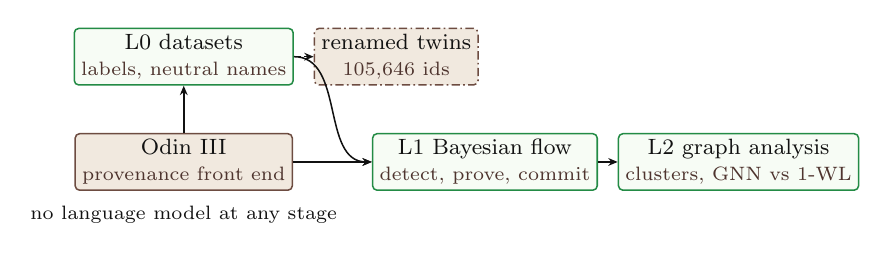
\begin{tikzpicture}[odin]
  % the base the pipeline stands on
  \node[box, neutral] (odin) {Odin III\\\odinsub{provenance front end}};
  % L0: datasets and their renamed twins
  \node[box, light, above=6mm of odin] (l0) {L0 datasets\\\odinsub{labels, neutral names}};
  \node[box, external, right=2.5mm of l0] (rn) {renamed twins\\\odinsub{105,646 ids}};
  % L1: Bayesian flow
  \node[box, light, right=10mm of odin] (l1) {L1 Bayesian flow\\\odinsub{detect, prove, commit}};
  % L2: graph analysis
  \node[box, light, right=2.5mm of l1] (l2) {L2 graph analysis\\\odinsub{clusters, GNN vs 1-WL}};
  % flow
  \draw[flow] (odin.north) -- (l0.south);
  \draw[flow, dash pattern=on 2.4pt off 1.4pt] (l0) -- (rn);
  \draw[flow] (l0.east) to[out=0, in=180] (l1.west);
  \draw[flow] (odin.east) -- (l1.west);
  \draw[flow] (l1) -- (l2);
  % a note: no LLM anywhere
  \node[plain, below=1.5mm of odin, font=\scriptsize\color{o3sub}] {no language model at any stage};
\end{tikzpicture}
}
\caption{The Loki~III pipeline. L0 compiles the benchmarks through Odin~III into provenance-tracked, labelled, anonymised datasets (and their renamed twins). L1 proposes and proves structures in a Bayesian flow that commits into the same IR. L2 reads the graphs back and scores clustering and a GNN against a 1-WL baseline. No stage has a language model.}
\label{fig:loki}
\end{figure}

\subsection{One design through the pipeline}
\label{sec:walk}

The steps below follow one design, the 4-bit comparator micro \code{bm\_DL\_4\_bit\_comparator}
(three comparison outputs), from source to score. Each step names the file or code that
defines it.

% Sources: docs/specs/2026-10-21-l0-dataset-design.md sections 4, 5.1-5.4, 6.1-6.7;
% docs/runbook-l0.md; docs/specs/2026-10-21-l1-hypotheses-design.md sections 3, 9, 11, 12;
% loki/odin.py (open_front, floor_script), loki/build.py (build_floor), loki/re/loop.py.
\begin{enumerate}
\item \emph{HDL to Odin~III with provenance.} \code{read\_verilog} and the common front
 elaborate the design. Every IR object keeps its source spans (\code{Node.sources()}, the
 only provenance the binding exposes). Before mapping, Loki snapshots every word-level cell
 (type, parameters, spans) and every instance site.
\item \emph{Map to the floor.} \code{lower} keeps each word cell's exact span on every gate
 it creates; \code{abc --lut 6} gives each LUT the union of the spans of its cone. A LUT
 that merges the three comparators therefore lists all three spans.
\item \emph{Join and label.} A final cell is matched to a word cell when the word's span set
 is a subset of the cell's. The primary match gives \code{construct\_type} (here \code{\$eq},
 \code{\$gt}, \dots); a cell with several matches is flagged (\code{n\_construct\_cells}
 above one) and a cell with none stays \code{unknown}: a label is an answer key, never a
 guess. The module path comes from the instance spans, bus name and bit index from net
 names and aliases (\code{AeqB[0]}), and the datapath or control role from a rule table.
\item \emph{Anonymise and write the L0 files.} Nets, cells and port bits get names
 \code{n}$k$ from one counter. Loki writes \code{netlist.blif} and \code{netlist.v},
 \code{graph.json} (nodes with features and labels, edges), \code{labels.csv} (one row per
 node), \code{words.json} (the word-level connectivity the scorer needs) and \code{key.json}.
 Only \code{key.json} holds original names; no analysis reads it.
\item \emph{Verify.} Odin~III's \code{equiv-check} compares the written BLIF with the
 floor's own netlist and the anonymised netlist with the original; both must read
 \code{equivalent} before the floor counts as built.
\item \emph{L1: normalise.} \code{loki re} reads \code{netlist.blif} (never \code{key.json})
 into a fresh Odin~III design, level~0, in which every logic cell is a function (a LUT by its
 truth table, a gate by its library function). On \code{f1} with hard cells the \code{unmap}
 pass runs on the working copy and its facts feed the \code{hard} detector.
\item \emph{L1: hypothesis rounds.} Each round runs the detectors, scores every hypothesis
 (Section~\ref{sec:bayes}), proves the ones worth a proof, resolves conflicts and commits the
 confident ones (Algorithm~\ref{alg:l1}); the next round sees the committed level.
\item \emph{L1: commit and output.} A committed hypothesis is rebuilt as a word cell
 (\code{raise}) wrapped in a module (\code{submod}) tagged with its kind, confidence and
 recovered function. At the fixed point Loki writes \code{design.v}, \code{overlay.json}
 (every hypothesis with its evidence) and \code{report.json}, and checks the final design
 against the input with \code{equiv-check}.
\item \emph{L2.} \code{loki analyze} reads \code{graph.json} only: structural features, four
 clusterings and a GNN (Section~\ref{sec:l2}).
\item \emph{Score.} \code{loki score} compares the overlay with the answer key
 (Section~\ref{sec:eval}); \code{loki score-all} aggregates every run into per-kind tables.
\end{enumerate}

In this micro the \code{f3} comparator, as re-synthesised by the minimal \code{.v} front, has 26 logic cells (L1 spec,
Section~3); the \code{f2} LUTs carry the comparator spans that the join reads back.

\subsection{Metrics and statistics}
\label{sec:metrics}

\emph{Recovery metrics.} Precision, recall and F1 (micro and macro) of the counted hypotheses
against the answer key; the expected calibration error (ECE); AST and CFG similarity and the
operator type-F1 of recovered text against the reference; modularity and NMI of a clustering;
the functional pass rate of recovered RTL; and the share of units lost at a pass. All are
defined in the Glossary and in Section~\ref{sec:eval}.

\emph{Area, speed and power.} Loki's measures are recovery measures. No experiment of this paper
measures area, speed (critical-path delay or near-critical paths) or power. We do not claim that
the recovery scores correlate with any of them, and we cite no work that says so; they are not
measured here.

\emph{Statistics.} Paired comparisons over designs use the Wilcoxon signed-rank test; paired
pass/fail comparisons use the exact two-sided McNemar test on discordant pairs; intervals are
bootstrap intervals (clustered over designs where the designs come in families); the null models
(random cell sets of the same size, random merges) are named where they are used. A result is
called a difference only when the interval or the exact test shows one; otherwise it is
INCONCLUSIVE.

\subsection{The language-model baseline: the Gate-Breaker metrics}
\label{sec:gb-results}

Gate-Breaker's metrics compare a recovered RTL against a reference: Success Rate,
Success@$k$, AST similarity and CFG similarity. Loki recovers structure, not a new RTL text,
so the direct comparison is the replication: the Gate-Breaker harness itself, run on the
simple benchmarks with the only language model available on the host, gave success rate
0.933 on Q1 and 0.829 on Q2, Success@10 1.000 in both quartiles, AST similarity 0.576 and
0.444, CFG similarity 1.000 and 0.736, with 169 of 174 extracted candidates functionally
correct -- a first replication on the fallback micro set, not the paper's VerilogEval set.
The VerilogEval replication, on the quartiles the paper used, is reported in
Table~\ref{tab:veval} with the AST and CFG kernels recomputed with common-width feature
vectors (the first run padded per graph and truncated in the zip, which the v1.1.0 CFG probe
found; those columns are not comparable to it).

\begin{table}[t]
\caption{Gate-Breaker metrics on the VerilogEval quartiles (one run, K=10, 4 workers, 180\,s
per call, 7,440\,s wall clock, 740 calls; deltas vs the paper's O3-Mini in the text).}
\label{tab:veval}
\centering
\footnotesize
\begin{tabular}{@{}lrrrrrr@{}}
\toprule
Quartile ($n$) & SR & S@1 & S@5 & S@10 & AST & CFG \\
\midrule
Q1 (36) & 0.903 & 0.944 & 1.000 & 1.000 & 0.894 & 0.942 \\
Q2 (37) & 0.778 & 0.811 & 1.000 & 1.000 & 0.761 & 0.890 \\
\bottomrule
\end{tabular}
\end{table}

This replication ran Q1 and Q2 only; the Loki-only results for Q3 and Q4 on the same designs are in
Section~\ref{sec:quartiles}. Seventy-four of the 78 Q1+Q2 designs are usable (three excluded because their synthesized
netlists fail the official testbench self-check, one because its 241\,KB prompt exceeds the
OS argument limit); every scored design is solved by attempt 5. The deltas against the
paper's O3-Mini: Q1 success rate -0.092, AST -0.030, CFG -0.011; Q2 success rate -0.039,
Success@5 +0.125, Success@10 +0.111, AST -0.164, CFG +0.083. The Q1 gap is harness
no-output, not wrong RTL; the Q2 AST gap is truth-table and case references against the
model's boolean expressions. Two caveats: the host's only model path routes through a
gateway that aliases a DeepSeek backend as Claude Opus (so the model column is not
verifiably the paper's comparison class), and the CLI exposes none of the paper's sampling
flags ($T{=}0.85$, $p{=}0.95$). The CFG column uses the common-width node kernel (the
odin3 CFG probe); the AST column uses the paper's pyverilog Algorithm~2 of Gate-Breaker.

What the two lines of work measure is complementary. The language model recovers functional
behaviour from the gates and names nothing reliably; Loki recovers the structures the flow
preserved (hard blocks, the hierarchy, the signal roles its features see) and proves what it
claims. The Gate-Breaker future work -- bus naming, datapath/control classification,
partitioning -- is exactly L2's table, and its numbers are the baseline a model-assisted
Loki would have to beat.

\subsection{The VerilogEval benchmark and its structure}
\label{sec:bench}

\subsubsection{VerilogEval spec-to-rtl as the Gate-Breaker benchmark}
\label{sec:veval-bench}

Gate-Breaker evaluates on VerilogEval~\cite{liu2023verilogeval}, taking the spec-to-rtl
variant: 156 problems, each a natural-language prompt, a reference solution
(\code{*\_ref.sv}, module \code{RefModule}) and a testbench (\code{*\_test.sv}). The
Gate-Breaker flow synthesizes the reference to a cmos6 gate netlist, hands the netlist to the
model, and checks the model's RTL against the testbench. Loki uses the same 156 references as
L0 sources and reads the reference module as the design; the prompts and testbenches are not
inputs to L0, L1 or L2. The references are SystemVerilog, read through Odin~III's slang
adapter (Section~\ref{sec:veval-l0}).

% Sources: work/gatebreaker-exp2/EXPERIMENT.md section 2 (156 *_ref.sv, *_test.sv, *_prompt.txt);
% work/gatebreaker-exp2/scripts/complexity.py (the score and its feature rules; weights and
% definitions below are quoted from its docstring and WEIGHTS table); experiments/veval-l0/
% EXPERIMENT.md Protocol step 3 (bins, 60 AST / 96 regex); experiments/veval-l0/complexity.csv
% (per-design score, quartile, method) -> Table tab:veval-bench.
\subsubsection{The complexity score and its quartiles}
\label{sec:complexity}

Gate-Breaker groups the problems by a complexity score (its Eq.~2), a weighted sum of
counts of HDL constructs:
\begin{multline}
C = 1000\,c_{\mathrm{Seq}} + 200\,(c_{\mathrm{FG}} + c_{\mathrm F}) + 20\,c_{\mathrm{Mo}}
 + 15\,(c_{@A} + c_{\mathrm B}) \\
 + 10\,(c_{\mathrm M} + c_{\mathrm{Ca}}) + 5\,c_{\mathrm E}
 + 3\,c_{\mathrm A} + 2\,c_{\mathrm C}.
\label{eq:complexity}
\end{multline}
The paper names the terms but does not define them, so the implementation we reuse
(\code{complexity.py} of the second Gate-Breaker replication) fixes the reading:
$c_{\mathrm{Seq}}$ counts clocked \code{always} blocks (a \code{posedge} or \code{negedge} in
the sensitivity list), $c_{\mathrm{FG}}$ for-generate constructs, $c_{\mathrm F}$ \code{for}
loops, $c_{\mathrm{Mo}}$ module instantiations, $c_{@A}$ all \code{always} blocks,
$c_{\mathrm B}$ declarations wider than one bit, $c_{\mathrm M}$ multiplexers (ternary
operators plus non-default \code{case} items), $c_{\mathrm{Ca}}$ \code{case} statements,
$c_{\mathrm E}$ arithmetic operators (\code{+ - * / \%}), $c_{\mathrm A}$ continuous
assignments and $c_{\mathrm C}$ concatenations. A clocked block weighs 1000 on its own, so a
design in which the counter recognises one scores at least 1000, which is Q3 or Q4.

The quartiles are the paper's absolute bins (its Table~II), not rank quartiles of the
benchmark: Q1 is 3 to 23, Q2 24 to 111, Q3 112 to 1064 and Q4 1065 to 1326. The 156 references
fall 38, 39, 40 and 39 into Q1 to Q4, close to the paper's 39 per quartile. The 150
designs that build on every floor are split 38, 39, 37 and 36: the six missing ones are
\code{Prob031}, \code{Prob046} and \code{Prob145} (Q3) and \code{Prob078}, \code{Prob151} and
\code{Prob156} (Q4). Table~\ref{tab:veval-bench} gives the counts.

\emph{Deviation: pyverilog AST against a regex fallback.} The score is computed on the
pyverilog AST of the first module when the file parses, and by regular-expression counts of
the same terms otherwise, with the method recorded per design. Because the references are
SystemVerilog, pyverilog parses only 60 of the 156; the other 96 use the regex counts. The
split is skewed by quartile (Table~\ref{tab:veval-bench}): 36 of Q1 and 23 of Q2 are
AST-scored, but 1 of Q3 and none of Q4. The regex counts operator characters and keywords
textually, so they differ from an AST count (the observed Q4 range, 1069 to 3259, exceeds the
paper's bin top of 1326 for this reason or because the problems differ; we do not separate the
two). The regex also never counts \code{always\_comb}, \code{always\_ff} or \code{always\_latch}
blocks, which 34 references use, so \code{c@A} and \code{cSeq} are undercounted in the 96
regex-scored designs, most of Q3 and Q4; the quartile split and the feature trends below rest on
approximate scores. The 156 scores equal those of the replication that computed them first, exactly, so the
quartiles here and in Table~\ref{tab:veval} are the same partition.

% Sources: experiments/veval-l0/EXPERIMENT.md "Feature rules" table and Caveats;
% experiments/veval-l0/features.csv; stats.json (feature_coverage).
\subsubsection{The feature matrix}
\label{sec:veval-features}

Gate-Breaker characterises its benchmark by the HDL structures it contains. We build the
same kind of matrix for the 150 built designs, from the \code{f3} floor of each, with
rules fixed in advance (\code{summarize.py}):
\emph{arithmetic} counts the word cells of type \code{\$add \$sub \$mul \$div \$mod \$neg
\$pos \$pow \$alu \$macc}; \emph{select/mux} those of type \code{\$mux \$pmux \$bmux \$demux};
\emph{storage} the register words (\code{\$dff}, \code{\$dffe}, \code{\$adff}, \code{\$adffe},
\code{\$sdff}, \code{\$sdffe}, \code{\$sdffce}, \code{\$dffsr}, \code{\$aldff},
\code{\$dlatch}, \code{\$adlatch}); \emph{FSM} is 1 when Odin~III's \code{fsm} pass marked any
word; \emph{control} is 1 when any label row has role \code{control} or \code{mixed}; and
\emph{wide buses} counts the distinct bus names with a bit index of at least 1. The matrix
uses one symbol per cell: \ding{55} for count 0, \ding{51} for one, \ding{51}\ding{51} for
two or more; FSM and control are 0/1 flags, so they show \ding{55} or \ding{51} only.

The bus column is \code{buses\_wide}, not \code{buses}. The latter counts every named signal,
including single-bit ports, so it is at least 1 for all 150 designs and at least 2 for 147,
and would put a check mark in every row. The wide count is the quantity a ``multi-bit bus''
row means; both columns are committed in \code{features.csv}.

Table~\ref{tab:veval-sample} shows 12 designs, three per quartile at fixed ranks by size, so
the sample is not hand-picked; Table~\ref{tab:veval-features} counts, per quartile, the
designs that show each feature. The storage trend is partly tautological: a clocked block adds 1000 to the score
(Eq.~\ref{eq:complexity}) and storage counts register words, so storage rises with the quartile
by construction; the other trends are conditioned on the score as well. Storage is absent from Q1 and Q2 (0 of 77 designs) and present in 31 of 37 Q3 and all 36 Q4
designs. The other features grow with the quartile: select/mux 8\% in Q1 to 56\% in Q4, control
3\% to 83\%, FSMs 0 of 77 below Q3 and 15 of 36 in Q4. Arithmetic is rare throughout (21 of
150, 14\%), so the benchmark leans on control, selection and storage more than on arithmetic
datapaths. Wide buses are common from Q2 up (90\%, 59\%, 100\%) but nearly absent in Q1
(8\%), whose members mostly have only single-bit signals. The FSM flag is Odin~III's detection, not a
reading of the source: \code{Prob107\_fsm1s} in Table~\ref{tab:veval-sample} has storage
and control cells but no FSM mark.

% Sources: experiments/veval-l0/sizes.csv and stats.json ("sizes"), via paper_tables.py;
% largest design, the count of designs at most 100 nodes and above 1000 nodes: benchmark.csv
% (f3_nodes column); micro f3 size: experiments/f3-recovery/EXPERIMENT.md (50,047 nodes, 65 designs).
\subsubsection{Benchmark size per technology mapping}
\label{sec:veval-sizes}

Table~\ref{tab:veval-sizes} gives the size of the 150 designs on each floor. The averages
hide a heavy tail. Over all designs the mean node count is 163.5 on \code{f1-k6}, 111.4 on
\code{f2} and 362.0 on \code{f3}, but the medians are 14.0, 13.5 and 25.0: most references
are small (125 of 150 have at most 100 nodes at \code{f3}) and a few are large (9 exceed
1000; the largest, \code{Prob144\_conwaylife}, has 15,487). The gate mapping multiplies
the node count of the LUT mapping by about 3 on the mean and 1.9 at the median (362.0 against 111.4 on average, 25.0 against 13.5 at the
median), as expected when a LUT of up to six inputs becomes a network of cells from a
library of one- and two-input gates (BUF, INV, NAND2, NOR2).
\code{f1-k6} sits above \code{f2} on average and in Q3 and Q4 (109.4 against 77.4; 453.9
against 269.8) while the two coincide in Q1 and Q2 (6.3 and 6.1; 100.2 and 100.0): the
\code{f1-k6} floor keeps hard cells (21 designs hold hard adders) where \code{f2} spreads
arithmetic over LUTs, which is consistent with the excess but is not isolated here. By quartile on \code{f3}, the mean grows from 9.9 nodes in Q1 to 972.1 in
Q4, but the Q4 median is only 51.5: the complexity score tracks the number and kind of HDL
constructs, not the netlist size. For scale, the micro suite's \code{f3} floors hold 50,047
nodes over 65 designs, a mean of about 770.

% Generated by experiments/veval-l0/paper_tables.py from benchmark.csv, complexity.csv,
% features.csv, sizes.csv and stats.json. Do not edit; rerun the script.

\begin{table}[t]
\caption{The VerilogEval spec-to-rtl references by Gate-Breaker complexity quartile (absolute bins of Table~II; score range observed in the 156 refs; pyverilog AST scores against regex-fallback scores; built = designs with all three floors).}
\label{tab:veval-bench}
\centering
\footnotesize
\begin{tabular}{@{}lrrrrrr@{}}
\toprule
Quartile & Bin & Observed & Refs & AST/regex & Built \\
\midrule
Q1 & 3--23 & 3--23 & 38 & 36/2 & 38 \\
Q2 & 24--111 & 24--90 & 39 & 23/16 & 39 \\
Q3 & 112--1064 & 120--1060 & 40 & 1/39 & 37 \\
Q4 & 1065--1326 & 1069--3259 & 39 & 0/39 & 36 \\
\midrule
All & & & 156 & 60/96 & 150 \\
\bottomrule
\end{tabular}
\end{table}

\begin{table}[t]
\caption{Benchmark feature matrix, a sample of 12 of the 150 designs (the designs at ranks $\lfloor n/6\rfloor$, $\lfloor n/2\rfloor$ and $\lfloor 5n/6\rfloor$ by f3 node count inside each quartile). \ding{55}: feature absent; \ding{51}: one; \ding{51}\ding{51}: more than one; FSM and control are 0/1 flags. Features are read from the f3 floor (Section~\ref{sec:veval-features}).}
\label{tab:veval-sample}
\centering
\scriptsize
\setlength{\tabcolsep}{3pt}
\begin{tabular}{@{}llrcccccc@{}}
\toprule
Design & Q & f3 nodes & Arith & Sel & Stor & FSM & Ctl & Bus \\
\midrule
Prob028\_m2014\_q4a & Q1 & 3 & \ding{55} & \ding{55} & \ding{55} & \ding{55} & \ding{55} & \ding{55} \\
Prob036\_ringer & Q1 & 8 & \ding{55} & \ding{55} & \ding{55} & \ding{55} & \ding{55} & \ding{55} \\
Prob091\_2012\_q2b & Q1 & 17 & \ding{55} & \ding{55} & \ding{55} & \ding{55} & \ding{55} & \ding{51} \\
\midrule
Prob125\_kmap3 & Q2 & 15 & \ding{55} & \ding{55} & \ding{55} & \ding{55} & \ding{55} & \ding{55} \\
Prob015\_vector1 & Q2 & 32 & \ding{55} & \ding{55} & \ding{55} & \ding{55} & \ding{55} & \ding{51}\ding{51} \\
Prob123\_bugs\_addsubz & Q2 & 166 & \ding{51}\ding{51} & \ding{51} & \ding{55} & \ding{55} & \ding{55} & \ding{51}\ding{51} \\
\midrule
Prob107\_fsm1s & Q3 & 11 & \ding{55} & \ding{51} & \ding{51} & \ding{55} & \ding{51} & \ding{55} \\
Prob117\_circuit9 & Q3 & 28 & \ding{51} & \ding{51} & \ding{51}\ding{51} & \ding{55} & \ding{51} & \ding{51} \\
Prob045\_edgedetect2 & Q3 & 89 & \ding{55} & \ding{55} & \ding{51}\ding{51} & \ding{55} & \ding{55} & \ding{51}\ding{51} \\
\midrule
Prob128\_fsm\_ps2 & Q4 & 30 & \ding{55} & \ding{55} & \ding{51} & \ding{51} & \ding{51} & \ding{51}\ding{51} \\
Prob140\_fsm\_hdlc & Q4 & 52 & \ding{55} & \ding{55} & \ding{51} & \ding{51} & \ding{51} & \ding{51} \\
Prob115\_shift18 & Q4 & 1121 & \ding{55} & \ding{51}\ding{51} & \ding{51}\ding{51} & \ding{55} & \ding{51} & \ding{51}\ding{51} \\
\bottomrule
\end{tabular}
\end{table}

\begin{table*}[t]
\caption{Designs showing each feature, per complexity quartile: count (percent of the quartile). The last column counts designs with two or more instances of the feature (always 0 for the 0/1 flags). Wide buses are distinct multi-bit buses; a design with only single-bit ports has none.}
\label{tab:veval-features}
\centering
\footnotesize
\begin{tabular}{@{}lrrrrrr@{}}
\toprule
Feature & Q1 ($n{=}38$) & Q2 ($n{=}39$) & Q3 ($n{=}37$) & Q4 ($n{=}36$) & All ($n{=}150$) & $\geq 2$ \\
\midrule
Arithmetic & 2 (5\%) & 4 (10\%) & 7 (19\%) & 8 (22\%) & 21 (14\%) & 9 \\
Select/mux & 3 (8\%) & 10 (26\%) & 12 (32\%) & 20 (56\%) & 45 (30\%) & 12 \\
Storage & 0 (0\%) & 0 (0\%) & 31 (84\%) & 36 (100\%) & 67 (45\%) & 12 \\
FSM & 0 (0\%) & 0 (0\%) & 1 (3\%) & 15 (42\%) & 16 (11\%) & 0 \\
Control & 1 (3\%) & 4 (10\%) & 15 (41\%) & 30 (83\%) & 50 (33\%) & 0 \\
Wide buses & 3 (8\%) & 35 (90\%) & 22 (59\%) & 36 (100\%) & 96 (64\%) & 55 \\
\bottomrule
\end{tabular}
\end{table*}

\begin{table}[t]
\caption{Benchmark size per technology-mapping floor, 150 designs: mean / median node count (top), and per complexity quartile (bottom; nodes). Nodes are all graph nodes of the floor netlist: primary inputs and outputs, constants, cells.}
\label{tab:veval-sizes}
\centering
\scriptsize
\setlength{\tabcolsep}{3pt}
\begin{tabular}{@{}lrrr@{}}
\toprule
All 150 designs & f1-k6 & f2 & f3 \\
\midrule
Nodes & 163.5 / 14.0 & 111.4 / 13.5 & 362.0 / 25.0 \\
Cells & 114.6 / 5.0 & 62.5 / 4.0 & 313.2 / 13.5 \\
Nets & 218.3 / 12.0 & 93.5 / 10.0 & 344.2 / 21.0 \\
\midrule
Nodes by quartile & f1-k6 & f2 & f3 \\
\midrule
Q1 ($n{=}38$) & 6.3 / 5.0 & 6.1 / 5.0 & 9.9 / 8.0 \\
Q2 ($n{=}39$) & 100.2 / 26.0 & 100.0 / 26.0 & 238.2 / 32.0 \\
Q3 ($n{=}37$) & 109.4 / 18.0 & 77.4 / 13.0 & 260.6 / 28.0 \\
Q4 ($n{=}36$) & 453.9 / 26.5 & 269.8 / 26.5 & 972.1 / 51.5 \\
\bottomrule
\end{tabular}
\end{table}


\section{Experiments}
\label{sec:experiments}
\label{sec:results}

One subsection per hypothesis that is USEFUL or POSSIBLY GOOD, and per INCONCLUSIVE answer that the
paper's question needs. Each states the hypothesis, the experiment, the result and the verdict.
DISMISSED and the remaining INCONCLUSIVE hypotheses are in the research log
(Appendix~\ref{app:log}). The experiments were run in rounds (0 to 6); a subsection names the round where
its text refers to one, and the appendix gives their order.

\subsection{Naming neutrality and the answer key (L0a, L0b)}
\label{sec:veval-l0}

\hev{Hypotheses.} L0a: the pipeline uses no names, so renaming every identifier changes no
result. L0b: the provenance answer key reconstructs the reference on every floor with no recovery step.

\hev{Experiment.} For L0a, every identifier of every netlist (105,646 identifiers across 269
netlists) is renamed through one permutation, L1 and L2 are run on the renamed and the base floors, and
the tokens are mapped back. For L0b, the answer key is counted on the 156 VerilogEval references.

\hev{Result.} % experiments/rename-l2/EXPERIMENT.md, hypotheses.md rows L0a and L0b
L0a: all 476 pairs of L1 runs are byte-identical (204, 204 and 68 sets); the L2 clusters are
identical on 271 of 272 partitions, and the one difference is a spectral nondeterminism that also
occurs between two runs of the base design. The protocol also exposed a rename-script defect
(library \code{.blackbox} model names were renamed, which silently removed every hard proposal on
renamed floors), which was fixed. L0b: all 54,306 gate nodes of the 150 designs that build carry a
label, a cell type and an HDL span; module coverage is 1.000 and signal coverage has geometric
mean 0.986; six of the 156 references do not build.


\emph{Detail of L0b.} The experiment is run on the 156 VerilogEval spec-to-rtl reference designs
(Section~\ref{sec:bench}) next to the micro suite. The experiment builds the three floors \code{f1-k6}, \code{f2} and
\code{f3} for every reference (\code{f1-earch} is not built; one architecture is enough
because \code{f2} and \code{f3} do not depend on it).

% All numbers in this subsection: experiments/veval-l0/EXPERIMENT.md (Result in one paragraph,
% Caveats, Numbers), experiments/veval-l0/stats.json (ceiling block) and
% experiments/veval-l0/l0-ceiling-veval.csv; micro column: experiments/f3-recovery/EXPERIMENT.md
% (L0 ceiling table), the capped 715/745 is computed from the signals and ref_signals columns of
% l0-ceiling-veval.csv (min per design), and docs/runbook-l0.md (F3 acceptance: 65 ok, 3 skipped, 0 non-equivalent).
\emph{Coverage of the build.} Of the 156 references, 150 build on all three floors, and
\code{loki check} reports zero errors on the assembled dataset. Two are skipped by Odin~III's
SystemVerilog reader: \code{Prob151\_review2015\_fsm} and \code{Prob156\_review2015\_fancytimer}
(both Q4), with \code{ODIN3\_ERR\_PARSE ... an explicit 4-bit cast is not supported}. Four
fail Loki's own equivalence gate and are recorded as failed rather than forced in:
\code{Prob031\_dff} (the reference initialises \code{q} to \code{1'hx}; the writer-versus-Odin~III
BLIF check reports \code{differs} on \code{f1} and \code{f2}, while \code{f3} was equivalent)
and \code{Prob046\_dff8p}, \code{Prob078\_dualedge} and \code{Prob145\_circuit8}, whose negedge
flip-flops make \code{equiv-check} return an error status for both comparisons. One design,
\code{Prob144\_conwaylife}, was killed by Wyrd's default 2\,GB step memory limit (peak 4.3\,GB)
and built after a rerun with an 8\,GB limit. Reading \code{.sv} sources needed two fixes in
Loki (SystemVerilog is read with \code{--nolatches} only, since \code{--vtr-compat} is refused
for it, and the slang adapter is registered with the process); both are in
\code{loki/odin.py} and apply to the experiment run.

\begin{table}[t]
\caption{The L0 ceiling on \code{f3}, micro suite and VerilogEval references. Both columns are
counts over all built designs; the last row is the per-design coverage of declared signals.}
\label{tab:l0-ceiling}
\centering
\footnotesize
\begin{tabular}{@{}lrr@{}}
\toprule
 & Micro & VerilogEval \\
\midrule
Source designs & 68 & 156 \\
Built on \code{f3} & 65 & 150 \\
Refused by the reader & 3 & 2 \\
Failed equivalence gate & 0 & 4 \\
Gate nodes, each with a label row & 50,047 & 54,306 \\
Rows with \code{cell\_type} and HDL span & 100\% & 100\% \\
Module scopes / reference modules & 112 / 113 & 150 / 150 \\
Leaf signal names / declared signals & 611 / 666 & 841 / 745 \\
Per-design signal coverage: median & 100\% & 100\% \\
\hspace{1em}minimum & 55.6\% & 75.0\% \\
\hspace{1em}geometric mean & -- & 0.986 \\
\bottomrule
\end{tabular}
\end{table}

\emph{The ceiling.} On \code{f3} the 150 designs have 54,306 gate nodes. Every node has a
label row, a \code{cell\_type} and an HDL span: the label, \code{cell\_type} and HDL coverage
have geometric mean 1.000 over designs. Label coverage is rows over nodes, so it shows that a row
exists, not that its fields are informative; unmatched cells stay \code{unknown}. The 150 module scopes of the 150 reference modules are
all present (module coverage 1.000). Signal coverage, the recovered leaf signal names over
the signals the reference declares, has geometric mean 0.986 (arithmetic mean 1.029): 120
designs are at exactly 1, 28 are below it, and 2 are above it, where flattened array elements
add names. The micro suite shows the same shape with a slightly lower ceiling (Table~\ref{tab:l0-ceiling}):
99.1\% of module scopes and 91.7\% of signal names (an aggregate ratio, where VerilogEval's
841 over 745 is inflated by those two designs; capped at each design's declared count it is
715 over 745, 96.0\%). The two sets agree on the message of
Section~\ref{sec:l1-results}: every node has a label row, a \code{cell\_type} and an HDL span,
and what the mapping erased is the signal names, not the label rows. (Label coverage counts rows,
not informative values: a cell that no rule matched keeps the value \code{unknown}.)

\emph{Caveats, reported with the numbers.} (i) \code{--nolatches} turns inferred-latch paths
into don't-care and \code{lower --async sync} turns asynchronous resets into synchronous clears,
so a built netlist can differ from the reference's behaviour even though Loki's own checks
(netlist against its anonymised twin and against Odin~III's writer) pass; the build gate
guarantees internal consistency, not equality with the reference. (ii) The reference module,
instance and signal counts come from pyverilog where it parses the reference (130 of the 150)
and from a regex fallback otherwise (20); the regex counts are approximate and the
reference signal count is the weakest number in this section. (iii) The same pyverilog limit
decides the complexity quartiles (Section~\ref{sec:complexity}). (iv) A train/test split by
design is fixed by the manifest rule (117 train, 33 test on \code{f3}); it is not used here,
where no model is fitted.

\hev{Verdict.} L0a \verdict{USEFUL}: naming is neutral, so nothing the pipeline recovers is an
artefact of a name. L0b \verdict{USEFUL}: the answer key covers every gate node and every reference
module; what the mapping erased is signal names, not label rows.

\subsection{L1: what the flow already reverse engineered, and what it erased (L1h, L1c, L1s)}
\label{sec:l1-results}

\hev{Hypotheses.} L1h: structures that the synthesis flow already reverse engineered (hard
adders and multipliers) are recovered almost perfectly. L1c: calibration makes the predicted
probabilities honest. L1s: the flow also recovers the structures that synthesis erased.

\hev{Experiment.} L1 runs on the renamed floors with a calibration fitted on the training
designs, and is scored against the answer key (precision, recall, macro-F1, ECE).

\hev{Result.} 
Table~\ref{tab:l1} reports L1 on the renamed floors (identical to base, as the neutrality
check requires). The head-line result is the \code{hard} detector: hard adders recover 67 of
67 with precision 0.985, hard multipliers 30 of 30, because the synthesis flow itself already
reverse engineered them and \code{unmap} says so. The rest is the honest difficulty: on f1
the calibrated macro-F1 is 0.354 (counted 271, matched 107, ground truth 688), with
\code{ff\_en} at 0.364, registers at 0.021 and muxes at 0.018; on f2 it is 0.108 (91/19/686),
with adders at F1 0.237 (precision 1.000, recall 0.134) and most other kinds near zero.
Without calibration the flow proposes far more and confirms little: f1 macro-F1 0.202 with
1,128 counted (323 of them declined-adder proposals), f2 0.075. Calibration is honest about
itself: ECE 0.217 calibrated against 0.650 uncalibrated.

\begin{table}[t]
\caption{L1 recovery on the renamed floors, per kind. Precision/recall/F1 against the L0
ground truth; calibrated (micro-fit) columns. The hard kinds recover from \code{unmap}
facts; the rest must be re-found from the gates.}
\label{tab:l1}
\centering
\footnotesize
\begin{tabular}{@{}lrrr@{}}
\toprule
Kind (f1) & Precision & Recall & F1 \\
\midrule
hard\_add & 0.985 & 1.000 & 0.993 \\
hard\_mul & 1.000 & 1.000 & 1.000 \\
ff\_en & -- & -- & 0.364 \\
register & -- & -- & 0.021 \\
mux & -- & -- & 0.018 \\
mux\_bit & -- & -- & 0.081 \\
\midrule
macro-F1 (all kinds) & & & 0.354 \\
\midrule
Kind (f2) & & & \\
\midrule
adder & 1.000 & 0.134 & 0.237 \\
subtractor & 1.000 & 0.074 & -- \\
mux\_bit & -- & -- & 0.100 \\
adder\_cin & -- & -- & 0.029 \\
macro-F1 (all kinds) & & & 0.108 \\
\bottomrule
\end{tabular}
\end{table}

\emph{The gate netlist (f3), hypothesis F3.} Gate-Breaker's own input is a cmos6 gate netlist, so we built
the f3 floor (65 of 68 micro designs; the gate reader refuses three hard-block sources) and asked whether L1
recovers structure from it. % experiments/f3-recovery/EXPERIMENT.md, hypotheses.md row F3
On the 15 f3 test designs (23,098 gate nodes) no construct is counted (0 of 144 ground-truth
instances, macro-F1 0.0) and no hypothesis is committed: the best calibrated confidence in any test
design is a bus at $p=0.764$, below the 0.9 commit threshold. Without calibration the detectors count
1,166 constructs for 2 matches (macro-F1 0.038), and 2,569 counted bus hypotheses match none of the 120
ground-truth buses. The answer key itself is complete at this floor: all 50,047 gate nodes carry a label
row, a cmos6 cell type and an HDL span. F3 is \verdict{DISMISSED}; it is the reason for the next
experiment.

\begin{table}[t]
\caption{Round-2 L1 (RQ-L1): recovery from the f3 gate netlist re-mapped to LUT6 against the native f2 floor, same 65 micro designs. \code{test} is the 15 held-out designs, \code{all} the 65. Calibration: the micro-fit f2 table (gate rows: the f3 table). Hard kinds excluded from counts and averages; macro-F1 averages the kinds with a counted prediction.}
\label{tab:r2-l1}
\centering
\footnotesize
\resizebox{\columnwidth}{!}{%
\begin{tabular}{@{}llrrrrrrr@{}}
\toprule
Netlist & Calib. & Split & Runs & Counted & Matched & GT & micro-F1 & macro-F1 \\
\midrule
f3 gate netlist & calibrated & test & 15 & 0 & 0 & 116 & 0.000 & 0.000 \\
 & uncalibrated & test & 15 & 1{,}166 & 2 & 116 & 0.003 & 0.038 \\
\midrule
f3 re-mapped to LUT6 & calibrated & test & 15 & 68 & 2 & 116 & 0.022 & 0.076 \\
 & calibrated & all & 65 & 92 & 14 & 580 & 0.042 & 0.062 \\
 & uncalibrated & test & 15 & 252 & 4 & 116 & 0.022 & 0.044 \\
 & uncalibrated & all & 65 & 921 & 31 & 580 & 0.041 & 0.049 \\
\midrule
f2 floor (native LUT6) & calibrated & test & 15 & 72 & 4 & 116 & 0.043 & 0.153 \\
 & calibrated & all & 65 & 88 & 16 & 579 & 0.048 & 0.095 \\
 & uncalibrated & test & 15 & 255 & 13 & 116 & 0.070 & 0.121 \\
 & uncalibrated & all & 65 & 930 & 32 & 579 & 0.042 & 0.070 \\
\bottomrule
\end{tabular}}
\end{table}


\emph{Hypothesis L1 of round 2: the f3 failure is the detectors' vocabulary and not missing information.} The L1 detectors read LUT covers,
and the f3 netlist is a cmos6 gate netlist. The hypothesis predicts that re-mapping the same gates into LUT6 recovers
close to the f2 rate. We read each f3 \code{netlist.blif} into Odin~III, run
\code{abc --lut 6}, and give the result to \code{loki re} as an f2 netlist. Odin~III drops
the cell names in \code{abc}, so each of the \rtLoneLuts{} LUTs is expanded back to the
gates it covers: a bit-parallel simulation signature matches its output to the f3 net of the
same function, and the cover is the cone of that net down to the matched inputs.
\rtLoneNoMatchFrac{} of the LUTs ABC resynthesised implement a function that is no f3 net;
they take the support-contained share of their consumers' covers, and \rtLoneEmpty{} are left
with an empty cover. The expanded hypotheses are then scored against the unchanged f3 key,
and the native f2 floor of the same \rtLoneDesigns{} designs, with the same calibration, is the
comparison (Table~\ref{tab:r2-l1}). On the gate netlist the calibrated flow matches
\rtLoneGateMatched{} of \rtLoneGateGt{} instances in the \rtLoneTestDesigns{} test designs. After the LUT6
re-map it matches \rtLoneLutMatchedTest{} (native f2: \rtLoneNativeMatchedTest{}), and over
all \rtLoneDesigns{} designs \rtLoneLutMatchedAll{} against \rtLoneNativeMatchedAll{} of \rtLoneGtAll{},
a micro-F1 ratio of \rtLoneAllRatio{} in-sample (the \rtLoneDesigns{} designs include the designs the f2
calibration was fitted on) against \rtLoneTestRatio{} on the held-out test split. The decision rule asked for a ratio of at least \rtLoneThr{} on both splits, so H1 is \rtLoneStatus{}. The in-sample recovery is
that of f2, on the same kinds (adders, subtractors, muxes), but the 15-design test split holds
only a handful of matches (\rtLoneLutMatchedTest{} against \rtLoneNativeMatchedTest{}), so its
ratio is noise in either direction. The result is consistent with the f3 failure being the
detectors' vocabulary and not missing information in the gates, but does not show it; the f2
level it would recover to is itself low.

\hev{Verdicts.} L1h \verdict{USEFUL}: hard adders 67 of 67 (precision 0.985) and hard multipliers 30 of 30,
because the synthesis flow itself reverse engineered them. L1c \verdict{USEFUL}: ECE 0.217 calibrated against
0.650 uncalibrated. L1s \verdict{INCONCLUSIVE}: the recovery is weak (macro-F1 0.354 on f1, 0.108 on f2) but no
threshold or baseline was set, so we do not call it a failure. The LUT6 re-map (round-2 hypothesis L1) is
\verdict{INCONCLUSIVE}: it reaches the f2 level in-sample but the held-out split has too few matches to decide.

\subsection{L2: clusters that carry the hierarchy, and a GNN that beats 1-WL (L2a, L2b)}
\label{sec:l2-results}

\hev{Hypotheses.} L2a: community methods find the designer's hierarchy and centroid methods do
not. L2b: a GNN with node, graphlet, WL and NPN features beats the 1-WL baseline.

\hev{Experiment.} Four clusterings of the 68 micro designs are scored against the known module
hierarchy; the GNN is trained on the labelled training designs and scored on 13 test designs
(3,932 test nodes), once.

\hev{Result.} 
Table~\ref{tab:l2} scores the four clusterings against the known module hierarchy. Louvain
leads (modularity 0.4220, NMI 0.1360); k-means and affinity propagation do not find the
hierarchy (negative modularity), which is itself a result: graph structure alone, without
the labels, favours the community methods. 271 of 272 partition records are identical
between base and renamed floors; the one difference exposed a determinism defect in the
spectral path (repeated runs on the same base design give modularities -0.0079, -0.0410 and
0.0252), reported as an open issue rather than hidden.

The GNN result answers the paper's question directly. A node-only GraphSAGE loses to the
1-WL baseline on real micros (macro-F1 0.2413 against 0.2711); combining node, graphlet, WL
and NPN features turns it around (0.3545 against 0.2711 on the earlier real-micro run), and
the full labelled run of this experiment gives test macro-F1 0.4241 against 0.2717
(accuracy 0.8863 against 0.8492, 3,932 test nodes across 13 designs). The features carry the
recovery, not the message passing alone.

\begin{table}[t]
\caption{L2 clustering against the known module hierarchy (68 designs, mean over the
renamed floors, identical to base). Modularity and NMI(module\_path) per method.}
\label{tab:l2}
\centering
\footnotesize
\begin{tabular}{@{}lrr@{}}
\toprule
Method & Modularity & NMI \\
\midrule
Louvain & 0.4220 & 0.1360 \\
Spectral & 0.3620 & 0.1378 \\
Affinity propagation & -0.2264 & 0.2708 \\
k-means & -0.2912 & 0.3220 \\
\bottomrule
\end{tabular}
\end{table}

\hev{Verdicts.} L2a \verdict{USEFUL}: Louvain modularity 0.4220 and NMI 0.1360, while k-means and affinity
propagation have negative modularity (a clear gap, with no test). L2b \verdict{POSSIBLY GOOD}: macro-F1 0.4241
against 0.2717 for 1-WL, but it is one run on one split of 13 designs with no interval, and the node-only GNN
loses to 1-WL (0.2413 against 0.2711); the claim is that the features carry the recovery, not that the
GNN generalises.

\subsection{An instrument that sees recovery, and where the language model stands (L7, RQ-L2)}
\label{sec:round2}

\hev{Hypotheses.} L7: a word-level operator F1 separates runs that AST and CFG similarity tie on.
RQ-L2: Loki's AST and CFG similarity is below the language model's on Q1 and Q2, does not stay flat
from Q1 to Q4, and Loki's output is formally equal to its input.

\hev{Experiment.} Round 2 is compute-only: no language-model call was made, and the
language-model figures are the round-1 Gate-Breaker replication, read again. Every number in this
subsection is a macro generated from the summary tables of \code{experiments/round2}. L7 rescored every run set with the operator type-F1
(Section~\ref{sec:newinstruments}); RQ-L2 ran \code{loki re} on all 150 VerilogEval netlists and
scored the output Verilog against the reference.

\hev{Result.} \emph{L7: are AST and CFG blind to what Loki recovers?} Table~\ref{tab:r2-l7} rescores every run set. The floors separate cleanly, which neither
AST nor CFG can show because both exist only on f3: type-F1 \rtLsevenTypeFonek{} on f1 (the
hard detector), \rtLsevenTypeFtwo{} on f2 and \rtLsevenTypeFthree{} on the f3 gates. On the
f3 test designs (Table~\ref{tab:r2-ties}) the calibrated and uncalibrated L1 runs tie on both
metrics, AST by \rtLsevenDAst{} and CFG by \rtLsevenDCfg{}, while operator type-F1 moves by
\rtLsevenDF{}; the flatten control raises AST by \rtLsevenFAst{} and CFG by \rtLsevenFCfg{}
and leaves the recovery record, hence the operator F1, unchanged (\rtLsevenFF{}). By the rule H7 is \rtLsevenStatus{}. The tie the rule was written for, the calibrated flow against
the L0-stop netlist (both add nothing to the text), does not separate: their operator type-F1
is $0$ against $0$. The verdict rests on the calibrated flow against the uncalibrated one,
where the calibrated side recovers no operator at all, and on the flatten clause, which holds
by construction. Two cautions: the separating level is small (the uncalibrated
detectors count mostly wrong constructs), and the flatten comparison holds the record fixed
by construction, because the operator F1 reads the recovery record and AST and CFG read the
text. The operator F1 does not replace them; it is the measure that sees recovery, where
they see only form.

\begin{table}[t]
\caption{Operator-recovery F1 (RQ-L7) of the existing and new L1 runs: the multiset of recovered operators (class and operand width) against the operators of the L0 key, pooled over designs. \code{type} ignores the width, \code{tw} requires it.}
\label{tab:r2-l7}
\centering
\footnotesize
\resizebox{\columnwidth}{!}{%
\begin{tabular}{@{}lrrrrrrr@{}}
\toprule
Run set & Designs & Key ops & Got ops & P & R & type-F1 & tw-F1 \\
\midrule
f1-k6, calibrated & 68 & 468 & 169 & 0.657 & 0.237 & 0.349 & 0.204 \\
f1-k6, none & 68 & 468 & 964 & 0.233 & 0.481 & 0.314 & 0.166 \\
f2, calibrated & 68 & 468 & 21 & 0.810 & 0.036 & 0.070 & 0.061 \\
f2, none & 68 & 468 & 756 & 0.180 & 0.291 & 0.222 & 0.080 \\
f3 gates, calibrated & 15 & 108 & 0 & -- & 0.000 & 0.000 & 0.000 \\
f3 gates, none & 15 & 108 & 1{,}161 & 0.009 & 0.102 & 0.017 & 0.008 \\
f3 as LUT6, calibrated & 65 & 463 & 19 & 0.895 & 0.037 & 0.071 & 0.062 \\
f3 as LUT6, none & 65 & 463 & 753 & 0.190 & 0.309 & 0.235 & 0.086 \\
VerilogEval f2, calibrated & 150 & 3{,}585 & 11 & 0.727 & 0.002 & 0.004 & 0.002 \\
VerilogEval f2, none & 150 & 3{,}585 & 1{,}151 & 0.196 & 0.063 & 0.095 & 0.042 \\
VerilogEval f3, calibrated & 150 & 3{,}585 & 2 & 1.000 & 0.001 & 0.001 & 0.001 \\
VerilogEval f3, none & 150 & 3{,}585 & 5{,}488 & 0.107 & 0.163 & 0.129 & 0.027 \\
\bottomrule
\end{tabular}}
\end{table}

\begin{table}[t]
\caption{AST and CFG similarity against operator F1 on the 15 f3 test designs (the f3-recovery runs). Calibrated and uncalibrated L1 tie on AST and CFG; the flatten control moves both and leaves the recovery record unchanged.}
\label{tab:r2-ties}
\centering
\footnotesize
\resizebox{\columnwidth}{!}{%
\begin{tabular}{@{}lrrrr@{}}
\toprule
Condition & AST & CFG & Ops recovered & type-F1 \\
\midrule
L0-stop gate netlist & 0.4044 & 0.6468 & 0 & 0.0000 \\
L1 calibrated & 0.4044 & 0.6468 & 0 & 0.0000 \\
L1 uncalibrated & 0.4155 & 0.6394 & 1{,}161 & 0.0173 \\
L1 uncalibrated, flattened & 0.4576 & 0.6941 & 1{,}161 & 0.0173 \\
\bottomrule
\end{tabular}}
\end{table}


\emph{RQ-L2: Loki against the language model on the same designs.} Round 1 scored the
language model on Q1 and Q2 of VerilogEval, and Loki's AST and CFG only on micro designs. We
ran \code{loki re} on all \rtLtwoDesigns{} VerilogEval netlists at f2 and f3, calibrated (a calibration
fitted on the \rtLtwoTrainDesigns{} train designs of VerilogEval itself) and not, and scored the output Verilog
(\code{design.v}) against the reference \code{.sv} with the round-1 AST and CFG code.
\rtLtwoRefAstFail{} references that pyverilog cannot parse have no AST value for any
candidate, and \rtLtwoCfgSkip{} f3 outputs exceed the CFG probe's size limit
(\code{l2\_coverage.csv}). On the designs both are scored on (Table~\ref{tab:r2-l2}), Loki's
f3 output has AST similarity \rtLtwoLokiAstQa{} in Q1 and \rtLtwoLokiAstQb{} in Q2 (common
designs, $n=\rtLtwoCommonNQa{}$ and $\rtLtwoCommonNQb{}$) against the model's \rtLtwoLlmAstQa{} and \rtLtwoLlmAstQb{}, and CFG similarity
\rtLtwoLokiCfgQa{} and \rtLtwoLokiCfgQb{} against \rtLtwoLlmCfgQa{} and \rtLtwoLlmCfgQb{};
every gap is significant by a paired Wilcoxon test (\code{l2\_paired.csv}). The calibration
was fitted on the train designs and these means cover all \rtLtwoDesigns{}, so we also give the held-out
test split alone (\code{l2\_testsplit.csv}): on its \rtLtwoTestN{} Q1 and Q2 designs both
tools score on, AST is \rtLtwoTestLokiAst{} for Loki against \rtLtwoTestLlmAst{} for the model
and CFG \rtLtwoTestLokiCfg{} against \rtLtwoTestLlmCfg{}, the same direction. (The calibrated
f3 flow commits in only \rtLtwoCommitDesigns{} designs, so the fit can change few outputs.) Across the four
quartiles (Table~\ref{tab:r2-l2q}) the f3 AST over all scored designs ($n=\rtLtwoTrendNQa{}$, \rtLtwoTrendNQb{}, \rtLtwoTrendNQc{}, \rtLtwoTrendNQd{}; a different, larger
design set than the common rows above) reads \rtLtwoTrendAstQa{}, \rtLtwoTrendAstQb{},
\rtLtwoTrendAstQc{} and \rtLtwoTrendAstQd{}, so it falls from Q1 to Q4 without being monotone. The \rtLtwoRefAstFail{} references that
do not parse fall in Q1 to Q4 as \rtLtwoRefFailQa{}, \rtLtwoRefFailQb{}, \rtLtwoRefFailQc{} and
\rtLtwoRefFailQd{}, so Q3 and Q4 are scored on the designs that parse, and the apparent fall
may partly reflect which designs those are. The CFG stays flat (\rtLtwoTrendCfgQa{} to \rtLtwoTrendCfgQd{}). The calibrated f3 flow
commits almost nothing, so its output is the L0 netlist; the uncalibrated flow, which does
commit, scores lower, not higher.

What the correctness column proves is narrow. Every one of the \rtLtwoEquivRuns{} runs of each
set ends \code{final\_equiv = equivalent} (\rtLtwoEquivOk{} for the calibrated f3 set), which
says that the flattened output is formally equal to the \emph{input netlist}. It does not say
the output matches the reference RTL: that netlist itself passes the official testbench in only
\rtLtwoSelfOk{} of the \rtLtwoDesigns{} designs (the round-1 self-check; inferred latches and asynchronous
resets are the failures), so Loki's output is exactly as correct as its input, no more. The
model is checked against the testbench directly, but only its correct samples enter the
similarity columns. On operator recovery (RQ-L7) the model is far ahead: on the common Q1 and
Q2 designs its operator type-F1 is \rtLtwoOpsLlm{} (functionally correct samples elaborated with
the same Odin~III front as the key) against \rtLtwoOpsLokiCal{} for Loki's calibrated f2 run and
\rtLtwoOpsLokiNone{} uncalibrated (the calibrated f3 run recovers no operator, 0.0, so the
comparison uses f2, a different floor from the one AST and CFG use). By the rule, H2 is \rtLtwoStatus: Loki is below the model
on both metrics in both quartiles (\rtLtwoCondA), the equivalence holds in all runs
(\rtLtwoCondC), and the similarity does not stay flat from Q1 to Q4 (\rtLtwoCondB). The
positioning this measures is that the model is readable and recovers the operators of small
designs but is unverified, and Loki is verified but partial; neither number alone is the
result, and the arm that combines them (a model given the ReverseProvenance record, L8) was
not run.

\begin{table}[t]
\caption{Head-to-head on the VerilogEval designs the language model was scored on (Q1 and Q2, functionally correct samples; AST depth 3 and CFG as in Table~\ref{tab:veval}). Loki columns: the output Verilog of the flow at that floor against the reference \code{.sv}; \code{L0} is the netlist before L1.}
\label{tab:r2-l2}
\centering
\footnotesize
\resizebox{\columnwidth}{!}{%
\begin{tabular}{@{}lrrrrrr@{}}
\toprule
Metric & LLM (round 1) & f3 netlist (L0) & f3 L1 cal. & f3 L1 none & f2 L1 cal. & f2 L1 none \\
\midrule
Q1 AST & 0.894 & 0.763 & 0.763 & 0.680 & 0.804 & 0.720 \\
Q1 CFG & 0.942 & 0.751 & 0.751 & 0.565 & 0.821 & 0.664 \\
Q2 AST & 0.761 & 0.460 & 0.460 & 0.438 & 0.459 & 0.448 \\
Q2 CFG & 0.890 & 0.743 & 0.743 & 0.679 & 0.787 & 0.764 \\
Q1+Q2 AST & 0.827 & 0.611 & 0.611 & 0.559 & 0.632 & 0.584 \\
Q1+Q2 CFG & 0.916 & 0.747 & 0.747 & 0.622 & 0.804 & 0.714 \\
\bottomrule
\end{tabular}}
\end{table}

\begin{table}[t]
\caption{Loki on all 150 VerilogEval designs by complexity quartile (mean AST and CFG of the output Verilog against the reference; last column: operator type-F1 of the uncalibrated f2 run). Calibrated f3 equals the f3 netlist wherever L1 commits nothing.}
\label{tab:r2-l2q}
\centering
\footnotesize
\resizebox{\columnwidth}{!}{%
\begin{tabular}{@{}lrrrrrrrr@{}}
\toprule
Quartile & $n$ & f3 AST & f3 CFG & f3 cal. AST & f3 cal. CFG & f2 cal. AST & f2 cal. CFG & op F1 \\
\midrule
Q1 & 38 & 0.754 & 0.750 & 0.754 & 0.750 & 0.793 & 0.820 & 0.061 \\
Q2 & 38 & 0.455 & 0.741 & 0.455 & 0.741 & 0.455 & 0.784 & 0.075 \\
Q3 & 32 & 0.614 & 0.751 & 0.605 & 0.750 & 0.607 & 0.811 & -- \\
Q4 & 21 & 0.505 & 0.768 & 0.505 & 0.768 & 0.507 & 0.870 & -- \\
\bottomrule
\end{tabular}}
\end{table}


\hev{Verdicts.} L7 \verdict{POSSIBLY GOOD}: the rule supports it, but the margins are small on few pairs (tie
pair $\Delta$F1 0.0173; the flatten control moves AST by 0.0422 and leaves the operator F1 unchanged), and the
calibrated flow recovers no operator at all, so we use the operator F1 only as an added instrument beside AST and CFG
and not as proof of an innovation. RQ-L2 \verdict{INCONCLUSIVE}: Loki is below the model on Q1 and Q2 (AST
0.763 and 0.460 against 0.894 and 0.761) and its output is equal to its input in 150 of 150 runs, but the AST falls
from Q1 to Q4, which may partly reflect which references parse, so the data position the two tools (the model readable
and unverified, Loki verified and partial) without deciding between them.

\subsection{Why the detectors miss: fragments and words (H9a, H9b)}
\label{sec:round3}

\hev{Hypotheses.} H9a: most false candidates are fragments of a word of a related kind. H9b: the
fragments of a word cover most of it, so grouping them recovers the word.

\hev{Experiment.} Uncalibrated, the detectors propose many candidates that almost never match
(Table~\ref{tab:r3-false}); calibrated, they commit almost nothing. Round 3 is compute-only on the round-2
runs and the L0 answer key (no language-model call, no new detector); every figure below is a macro
generated from the summary CSVs of \code{experiments/round3}. The round-2 counts that motivate the question
(for instance \code{ff\_en} 732 candidates and one correct on the held-out designs) were known when the
thresholds were set. Analyses added after the data was seen are labelled \emph{exploratory} and decide
nothing. We added the runs the round-2 sets lacked (micro f3, calibrated and not, and micro f1-k6,
uncalibrated; one micro f3 design timed out) and score every set, but the decisions use the primary set P:
the micro and VerilogEval f2 runs without calibration.

\begin{table}[t]
\caption{RQ-L9, primary set P (M2N+V2N, f2, uncalibrated): counted candidates, false ones, and the share of the false ones per class (rules of \code{EXPERIMENT.md}).}
\label{tab:r3-false}
\centering
\footnotesize
\resizebox{\columnwidth}{!}{%
\begin{tabular}{@{}lrrrrrrrr@{}}
\toprule
kind & cand. & false & same ext. & frag. rel. & frag. other & straddle & partial & noise \\
\midrule
ff\_en & 1{,}070 & 1{,}067 & 0.01 & 0.99 & 0.00 & 0.00 & 0.00 & 0.00 \\
mux\_bit & 344 & 336 & 0.00 & 0.61 & 0.39 & 0.00 & 0.00 & 0.00 \\
eq\_const & 1{,}105 & 1{,}096 & 0.00 & 0.18 & 0.82 & 0.00 & 0.00 & 0.00 \\
register & 155 & 116 & 0.03 & 0.64 & 0.15 & 0.19 & 0.00 & 0.00 \\
\bottomrule
\end{tabular}}
\end{table}

\begin{table}[t]
\caption{RQ-L9 (H9b), set P: ground-truth instances with at least two cells, the share whose fragment union covers at least 0.8 of them ($q$), the same with candidates of any kind, and the mean fragment coverage.}
\label{tab:r3-frag}
\centering
\footnotesize
\resizebox{\columnwidth}{!}{%
\begin{tabular}{@{}lrrrrr@{}}
\toprule
kind & GT & matched & $q$ frag. & $q$ any & mean cov. \\
\midrule
ff\_en & 156 & 3 & 0.122 & 0.160 & 0.618 \\
mux\_bit & 368 & 2 & 0.005 & 0.136 & 0.016 \\
eq\_const & 995 & 5 & 0.040 & 0.112 & 0.089 \\
register & 289 & 39 & 0.194 & 0.228 & 0.497 \\
\bottomrule
\end{tabular}}
\end{table}

\begin{table}[t]
\caption{RQ-L9 for every run set (four decisive kinds pooled): runs, candidates, false candidates and the share that are related fragments, other-type fragments, noise.}
\label{tab:r3-sets}
\centering
\footnotesize
\resizebox{\columnwidth}{!}{%
\begin{tabular}{@{}lrrrrrr@{}}
\toprule
set & runs & cand. & false & frag. rel. & frag. other & noise \\
\midrule
M2N & 65 & 705 & 686 & 0.28 & 0.69 & 0.00 \\
M2C & 65 & 71 & 65 & 0.95 & 0.05 & 0.00 \\
V2N & 150 & 1{,}969 & 1{,}929 & 0.69 & 0.30 & 0.00 \\
V2C & not run &  &  &  &  &  \\
V3N & 150 & 5{,}005 & 4{,}997 & 0.29 & 0.71 & 0.00 \\
V3C & 150 & 2 & 0 & 0.00 & 0.00 & 0.00 \\
M3N & 64 & 1{,}406 & 1{,}405 & 0.23 & 0.77 & 0.00 \\
M3C & not run &  &  &  &  &  \\
M1N & 68 & 496 & 469 & 0.38 & 0.57 & 0.00 \\
\bottomrule
\end{tabular}}
\end{table}

\begin{table}[t]
\caption{Exploratory, non-deciding additions (2026-10-24, after the data), set P: share of false candidates that are related fragments (by candidate, by distinct cell), the noise$'$ share (cells only in plain-gate ground-truth words), $q$ over all words and over the words touched by a candidate.}
\label{tab:r3-expl}
\centering
\footnotesize
\resizebox{\columnwidth}{!}{%
\begin{tabular}{@{}lccccc@{}}
\toprule
kind & frag. rel. & frag. rel. (cells) & noise$'$ & $q$ & $q$ touched \\
\midrule
ff\_en & 0.99 & 0.98 & 0.00 & 0.122 & 0.123 \\
mux\_bit & 0.61 & 0.61 & 0.01 & 0.005 & 0.006 \\
eq\_const & 0.18 & 0.18 & 0.52 & 0.040 & 0.042 \\
register & 0.64 & 0.49 & 0.00 & 0.194 & 0.229 \\
pooled & 0.58 & 0.56 & 0.22 & 0.065 & 0.069 \\
\bottomrule
\end{tabular}}
\end{table}


\hev{Result.} A false candidate is a counted
candidate the one-to-one scorer does not match. We classify each (rules in the protocol): the
same extent as a ground-truth instance of its family (a lost tie or a type slip), a fragment
of a larger instance of its family, a fragment of an instance of another type, a straddle of
several, a partial overlap, or noise. Over the \rttNinePoolFalse{} false candidates of the four
kinds in P, \rttNinePoolFrag{} (\rttNinePoolFragN) are fragments of an instance of the matching or a
related family. Per kind the related-fragment share is \rttNineFfenFrag{} for \code{ff\_en},
\rttNineRegisterFrag{} for \code{register}, \rttNineMuxbitFrag{} for \code{mux\_bit} and only
\rttNineEqconstFrag{} for \code{eq\_const}; \rttNineKindsOk{} of four kinds reach 0.5, so H9a is
\rttLNineaStatus{} \emph{by the letter of the rule; not robust}. Three qualifications go with it.

First, the noise class is vacuous. The ground-truth instances cover every non-I/O, non-constant
cell of the f2 datasets (9{,}381 of 9{,}381 in VerilogEval, 9{,}130 of 9{,}130 in the micro set), so
rule 6 of the protocol could never yield noise, and the noise share \rttNinePoolNoise{} is
structural. The arm of the H9a rule that reads ``not supported when the noise share is at least
0.5'' was unreachable by construction, and the sentence that no wrong candidate is noise carries
no information. As an exploratory replacement we count noise$'$: a false candidate all of whose
cells lie only in plain-gate ground-truth words (\code{\$and}, \code{\$or}, \code{\$not},
\code{\$xor}, \code{\$xnor}, the \code{\$logic} and \code{\$reduce} gates). Pooled, noise$'$ is
\rttNineNoisePrime{} (\rttNineNoisePrimeN{} candidates); per kind it is \rttNineEqconstNoisePrime{} for
\code{eq\_const}, \rttNineMuxbitNoisePrime{} for \code{mux\_bit}, and \rttNineFfenNoisePrime{} for
\code{ff\_en} and \rttNineRegisterNoisePrime{} for \code{register} (Table~\ref{tab:r3-expl}).
Half of the false \code{eq\_const} candidates are thus glue logic, not a piece of a word.

Second, the \code{ff\_en} fragments are near-tautological. An \code{ff\_en} candidate has two
cells (a flip-flop and its enable LUT), and the ground-truth footprint of a register or
\code{\$dffe} word is the whole word, so a correct per-bit slice of a word counts as a fragment
of it; \rttNineFfenFragN{} of the \rttNinePoolFragN{} related fragments are \code{ff\_en}. For
\code{ff\_en} the detector finds correct bit slices and the miss is word-level grouping and
extent. Without \code{ff\_en} (exploratory) the pooled related-fragment share over the other
three kinds is \rttNineNoFfenFrag{} (\rttNineNoFfenFalse{} false candidates, \rttNineNoFfenKindsOk{} of
three kinds at or above 0.5), and \rttNineNoFfenTopFrag{} when the largest design is also left out. For
\code{mux\_bit} and \code{register} the fragment reading holds at the stated shares; for
\code{eq\_const} it is a detector problem: \rttNineEqconstOther{} of its false candidates are
fragments of an instance of another type (mostly single-LUT \code{\$and} and \code{\$or} words,
registers and \code{fsm} instances), so the LUT computes something that looks like a constant
compare and is not one. The \code{mux\_bit} candidates are \rttNineMuxbitOther{} inside an
instance of another type (\code{\$shiftx} words among them).

Third, the result rests on one design. Most \code{ff\_en} candidates come from
\code{\rttNineTopDesign}, where they sit inside a mux tree, and overlapping candidates inflate
their count. With that design left out (exploratory, not the rule) \rttNineTopFalse{} false
candidates remain, \rttNineTopFrag{} of them related fragments and \rttNineTopOther{} fragments of
another type, so the pooled share falls under the 0.5 of the rule and H9a would be inconclusive;
\code{ff\_en} stays at \rttNineTopFfenFrag{} and \code{register} drops to
\rttNineTopRegisterFrag. Counted over the \rttNineCells{} distinct (design, cell) pairs covered by
false candidates instead of over candidates (exploratory), the pooled related-fragment share is
\rttNineCellFrag. We therefore state H9a with both numbers: \rttLNineaStatus{} by the letter of the
rule at \rttNinePoolFrag, not robust (\rttNineTopFrag{} without \code{\rttNineTopDesign},
\rttNineNoFfenFrag{} without \code{ff\_en}).

H9b asks whether grouping the fragments would recover the word: the share of ground-truth
instances whose fragment union covers 0.8 of them is
\rttNinePoolQ{} pooled (\code{ff\_en} \rttNineFfenQ, \code{register} \rttNineRegisterQ,
\code{eq\_const} \rttNineEqconstQ, \code{mux\_bit} \rttNineMuxbitQ), and no kind reaches 0.5, so
H9b is \rttLNinebStatus. The denominator holds words no candidate touched; over the
\rttNinePoolTouched{} words touched by at least one candidate (exploratory) the share is
\rttNinePoolQTouched. The shortfall is therefore detector misses plus non-tiling, not one of them:
\rttNinePoolQ{} of all words, \rttNinePoolQTouched{} of the touched ones. Even with candidates of any
kind the cover stays low (\code{register} \rttNineRegisterAny, \code{mux\_bit} \rttNineMuxbitAny).
The fragments exist, but they do not tile the words: a merge step over the present detector
output would recover few words. The other sets (Table~\ref{tab:r3-sets}) have fewer candidates
when calibrated, and the gate floor f3 proposes far more false \code{eq\_const} candidates than
any f2 set.

\begin{table}[t]
\caption{RQ-L11, ground truth: feedback registers, constant-compare decoders on them, sinks (mux selects and enables) and chains, and the muxes with a select (enabled words) whose select (enable) is a chain sink.}
\label{tab:r3-chain}
\centering
\footnotesize
\resizebox{\columnwidth}{!}{%
\begin{tabular}{@{}llrrrrrrrrrr@{}}
\toprule
dataset & floor & designs & with fb. & with chain & fb. reg. & fsm flag & decoders & sinks & chains & mux S chain/all & enable chain/all \\
\midrule
micro & f2 & 68 & 3 & 1 & 3 & 0 & 11 & 3 & 12 & 3/41 & 0/3 \\
micro & f3 & 65 & 3 & 1 & 3 & 0 & 11 & 3 & 12 & 3/41 & 0/3 \\
micro & f1-k6 & 68 & 3 & 1 & 3 & 0 & 11 & 3 & 12 & 3/41 & 0/3 \\
veval & f2 & 150 & 55 & 12 & 197 & 16 & 41 & 30 & 89 & 15/43 & 15/152 \\
veval & f3 & 150 & 55 & 12 & 197 & 16 & 41 & 30 & 89 & 15/43 & 15/152 \\
\bottomrule
\end{tabular}}
\end{table}

\begin{table}[t]
\caption{RQ-L11, detectors: chain elements proposed by a counted candidate with Jaccard at least 0.5 of any kind (in brackets: of the right scored type), chains with all three elements proposed, and ground-truth FSM instances matched by an \code{fsm} candidate.}
\label{tab:r3-detect}
\centering
\footnotesize
\resizebox{\columnwidth}{!}{%
\begin{tabular}{@{}lccccc@{}}
\toprule
set & fb. register & decoder & sink & complete chains & fsm \\
\midrule
M2N & 0/3 (0) & 1/11 (0) & 1/3 (0) & 0/12 (0) & 0/0 \\
M2C & 0/3 (0) & 0/11 (0) & 0/3 (0) & 0/12 (0) & 0/0 \\
V2N & 41/197 (26) & 15/41 (9) & 5/30 (0) & 5/89 (0) & 6/16 \\
V2C & 3/197 (0) & 1/41 (0) & 2/30 (0) & 1/89 (0) & 0/16 \\
V3N & 13/197 (3) & 6/41 (2) & 3/30 (0) & 4/89 (0) & 3/16 \\
V3C & 4/197 (0) & 2/41 (0) & 2/30 (0) & 2/89 (0) & 1/16 \\
M3N & 0/3 (0) & 0/11 (0) & 0/3 (0) & 0/12 (0) & 0/0 \\
M3C & 0/3 (0) & 0/11 (0) & 0/3 (0) & 0/12 (0) & 0/0 \\
M1N & 0/3 (0) & 0/11 (0) & 0/3 (0) & 0/12 (0) & 0/0 \\
\bottomrule
\end{tabular}}
\end{table}


\emph{RQ-L11: the FSM chain.} Measurement only. In the f2 ground truth of VerilogEval
(\rttElevenVeDesigns{} designs) \rttElevenVeFb{} registers feed back to themselves, of which
\rttElevenVeFsm{} the front end flags as FSM state; \rttElevenVeDec{} constant-compare decoders
read such a register, and the chains (register, decoder, select or enable) occur in
\rttElevenVeDesignsChain{} designs. Of the muxes with a select, \rttElevenVeMuxChain{} of
\rttElevenVeMuxS{} (VerilogEval) and \rttElevenMiMuxChain{} of \rttElevenMiMuxS{} (micro) take it from
such a decoder, \rttElevenMuxShare{} together, so the FSM, decode, select chain is real but covers a
minority of the control muxes of these small designs. The detectors see little of it
(Table~\ref{tab:r3-detect}): in V2N they propose \rttElevenVtwoNFb{} feedback registers,
\rttElevenVtwoNDec{} decoders, \rttElevenVtwoNSink{} sinks, all three elements of
\rttElevenVtwoNChain{} chains, and \rttElevenVtwoNFsm{} FSM instances as an \code{fsm} candidate.
The chains are triples (register, decoder, sink) and reuse their elements: the \rttElevenVeChains{}
triples hold only \rttElevenVeSinks{} distinct sinks and \rttElevenVeDec{} distinct decoders. Counted
on distinct elements, the detectors propose \rttElevenVtwoNSink{} of the sinks and
\rttElevenVtwoNDec{} of the decoders, against \rttElevenVtwoNChain{} complete triples.

\emph{Implication for a word-first detector.} The classification cannot say that the wrong
candidates are not noise, because the ground truth covers every cell and the noise class was
unreachable; the exploratory noise$'$ share is \rttNineNoisePrime{} pooled and \rttNineEqconstNoisePrime{} for
\code{eq\_const}. The fragment share depends on the kind and, for the pooled figure, on one design
and on the \code{ff\_en} slices: \code{ff\_en}, \code{mux\_bit} and
(less so) \code{register} fail as pieces of larger constructs, while \code{eq\_const} fails as
a detector problem (the local pattern is too weak, and a word-level view, the select and enable
fan-out across a word, must decide whether a compare is a decoder). Because the fragments do
not tile the words, grouping the present candidates is not enough, and a detector should
construct the word first and score it as a unit. Concretely, we propose to find (i) register words by shared clock, enable and reset
across flip-flops; (ii) datapath words by per-bit cones that are NPN-isomorphic, seeded from the
ports but not limited to them (the port words reach registers and nothing past the first
layer); (iii) control nets by select and enable fan-out across a word; and (iv) FSMs by a
feedback strongly connected component plus the decoders on it. Related work attacks the word
problem along the same lines: WordRev~\cite{li2013wordrev} derives word-level structures from
the gate-level netlist of a circuit and lets the user specify sequences of word-level operations
whose gates it then extracts, and DANA~\cite{albartus2020dana} recovers high-level registers by
analysing the flow of data between individual flip-flops. We ran DANA (through HAL~\cite{hal}) on the round-5 sets
(Section~\ref{sec:hal}); WordRev was not run and no comparison with it is claimed. The
next round builds this detector (L8, the language model given the ReverseProvenance record,
stays deferred).

\hev{Verdicts.} H9a \verdict{POSSIBLY GOOD}: by the letter of the rule about half of the false candidates are
fragments of a related kind (0.583 pooled), but the result fails leaving out one design (0.415) and the
near-tautological \code{ff\_en} slices (0.304), so we state it only with that fragility. H9b \verdict{DISMISSED}:
a word's fragments cover it in 0.065 of the words, so the fragments exist but do not tile the words; this is
the motive for the word-first detector of the next subsection. The FSM chain is a measurement and has no verdict.

\subsection{The word-first detector and DANA (H16a--H16f, RQ-H1)}
\label{sec:round5}

\hev{Hypotheses.} The word-first detector, built from the two lessons of the fragment study, makes
six claims: H16a, word tiling beats the earlier detectors on held-out real designs; H16b, grouping by clock,
enable and reset recovers the enabled-register words; H16c, a word-level \code{eq\_const} beats the per-bit
one; H16d, the FSM-decode-select chain is completed more often; H16e, words grown from registers reach the
datapath beyond a size-matched null; H16f, repetition is evidence on big designs. RQ-H1: the detector recovers
register words better than, equal to, or worse than DANA.

The fragment study says what to build: words from structure. Round 5 builds it (can words, control nets and FSMs be found first, and the rest built around them?). Two opt-in
detectors, \code{wordfirst} and \code{wordgroup} (\code{loki/re/detectors/wordfirst.py},
\code{docs/user/wordfirst.md}), were added to \code{loki re}; the default detector list and every
earlier calibration are unchanged. \code{wordfirst} groups flip-flops by clock, enable and reset
into register words (with \code{ff\_en} and \code{ff\_srst} words labelled by the control net),
groups 2:1 mux cells by their shared select, takes the carry chains of the \code{arith} detector
so that the carry net joins the bits, decides \code{eq\_const} at word level (a single-minterm
cone whose support lies in one register word or the primary inputs), proposes an FSM for a
register word coupled through its own D cones, and grows words along isomorphic bit slices
(readers and drivers) across registers, mux words and adders into \code{bus} words.
\code{wordgroup} runs last and links the per-bit hypotheses to the words that contain them. The
outputs are ordinary candidates with claims, so the prover, the commit step, the scorers and the
Verilog writer work unchanged. Every threshold is an agent default (no fitted parameter): groups
above 32 flip-flops are split by the Q-reader and D-driver signature, \code{eq\_const} supports
are at most 16, growth needs 0.75 of the bits and two levels.

The evaluation sets are the micros (MI), the
33 held-out VerilogEval designs (VT), the corpus iid and ood test splits (CI, CO) and the 13 big
designs that built at f2 (BIG). The arms are the round-2 detectors uncalibrated and calibrated
(R2N, R2C), \code{wordfirst} alone (W) and \code{wordfirst} with the per-bit detectors and
\code{wordgroup} (WB); all runs are uncalibrated. 

\begin{table}[t]
\caption{Round 5: word tiling q (share of GT words whose fragments cover 0.8) at f2.}
\label{tab:r5-tiling}
\centering
\footnotesize
\resizebox{\columnwidth}{!}{%
\begin{tabular}{@{}lrrrrrr@{}}
\toprule
Set & R2N & R2C & W & WB & null W & null WB \\
\midrule
MI & 0.212 & 0.019 & 0.223 & 0.237 & 0.042 & 0.048 \\
VT & 0.022 & 0.004 & 0.017 & 0.023 & 0.017 & 0.203 \\
CI & 0.390 & 0.328 & 0.312 & 0.397 & 0.206 & 0.294 \\
CO & 0.259 & 0.182 & 0.180 & 0.266 & 0.089 & 0.155 \\
\bottomrule
\end{tabular}}
\end{table}

\begin{table}[t]
\caption{Round 5, floor f2: precision/recall/F1 per kind and set for the round-2 detectors (R2N, R2C) and the word-first arms (W, WB). Pooled over the designs each arm has; GT is the first arm's count.}
\label{tab:r5-f2}
\centering
\footnotesize
\resizebox{\columnwidth}{!}{%
\begin{tabular}{@{}llrcccc@{}}
\toprule
Set & Kind & GT & R2N & R2C & W & WB \\
\midrule
CI & adder & 49 & 1.00/0.14/0.25 & 1.00/0.14/0.25 & 1.00/0.14/0.25 & 1.00/0.14/0.25 \\
CI & comparator & 167 & 0.00/0.00/0.00 & 0.00/0.00/0.00 & 0.00/0.00/0.00 & 0.00/0.00/0.00 \\
CI & counter & 10 & 0.62/0.50/0.56 & 1.00/0.60/0.75 & 0.00/0.00/0.00 & 0.62/0.50/0.56 \\
CI & eq\_const & 161 & 0.02/0.02/0.02 & 1.00/0.02/0.04 & 0.04/0.02/0.02 & 0.02/0.02/0.02 \\
CI & ff\_en & 78 & 0.00/0.00/0.00 & 0.00/0.00/0.00 & 0.20/0.18/0.19 & 0.02/0.18/0.03 \\
CI & ff\_srst & 70 & 0.00/0.00/0.00 & 0.00/0.00/0.00 & 0.31/0.39/0.35 & 0.04/0.37/0.07 \\
CI & fsm & 20 & 0.89/0.80/0.84 & 1.00/1.00/1.00 & 0.09/0.05/0.06 & 0.58/0.75/0.65 \\
CI & mux & 106 & 0.73/0.08/0.14 & 1.00/0.07/0.12 & 0.67/0.06/0.10 & 0.40/0.08/0.13 \\
CI & mux\_tree & 19 & 0.00/0.00/0.00 & 0.00/0.00/0.00 & 0.00/0.00/0.00 & 0.00/0.00/0.00 \\
CI & register & 163 & 0.57/0.37/0.45 & 0.59/0.26/0.36 & 0.27/0.30/0.29 & 0.36/0.40/0.38 \\
CI & subtractor & 32 & 0.50/0.09/0.16 & 1.00/0.09/0.17 & 1.00/0.09/0.17 & 0.50/0.09/0.16 \\
CO & adder & 90 & 0.22/0.02/0.04 & 0.22/0.02/0.04 & 0.30/0.03/0.06 & 0.22/0.02/0.04 \\
CO & comparator & 502 & 0.03/0.01/0.01 & 1.00/0.01/0.01 & 0.00/0.00/0.00 & 0.03/0.01/0.01 \\
CO & counter & 13 & 1.00/0.08/0.14 & 1.00/0.08/0.14 & 0.00/0.00/0.00 & 1.00/0.08/0.14 \\
CO & eq\_const & 491 & 0.01/0.01/0.01 & 0.33/0.01/0.02 & 0.01/0.01/0.01 & 0.01/0.01/0.01 \\
CO & ff\_en & 171 & 0.00/0.00/0.00 & 0.00/0.00/0.00 & 0.24/0.22/0.23 & 0.02/0.22/0.03 \\
CO & ff\_srst & 87 & 0.00/0.00/0.00 & 0.00/0.00/0.00 & 0.20/0.51/0.29 & 0.02/0.48/0.04 \\
CO & fsm & 40 & 0.88/0.53/0.66 & 1.00/0.97/0.99 & 0.06/0.03/0.04 & 0.54/0.53/0.53 \\
CO & mux & 213 & 0.32/0.08/0.13 & 0.94/0.08/0.15 & 0.46/0.03/0.05 & 0.49/0.08/0.14 \\
CO & mux\_tree & 32 & 0.00/0.00/0.00 & 0.00/0.00/0.00 & 0.00/0.00/0.00 & 0.00/0.00/0.00 \\
CO & register & 304 & 0.52/0.37/0.43 & 0.57/0.28/0.38 & 0.29/0.34/0.31 & 0.36/0.42/0.39 \\
CO & subtractor & 38 & 0.17/0.03/0.05 & 1.00/0.03/0.05 & 1.00/0.03/0.05 & 0.20/0.03/0.05 \\
MI & adder & 62 & 1.00/0.13/0.23 & 1.00/0.11/0.20 & 0.75/0.13/0.23 & 1.00/0.13/0.24 \\
MI & comparator & 116 & 0.01/0.01/0.01 & 0.00/0.00/0.00 & 0.00/0.00/0.00 & 0.01/0.01/0.01 \\
MI & counter & 2 & 0.00/0.00/0.00 & 0.00/0.00/0.00 & 0.00/0.00/0.00 & 0.00/0.00/0.00 \\
MI & eq\_const & 102 & 0.00/0.00/0.00 & 0.00/0.00/0.00 & 0.00/0.00/0.00 & 0.00/0.00/0.00 \\
MI & ff\_en & 4 & 0.04/0.50/0.07 & 0.00/0.00/0.00 & 0.14/0.25/0.18 & 0.05/0.75/0.09 \\
MI & ff\_srst & 9 & 0.00/0.00/0.00 & 0.00/0.00/0.00 & 0.11/0.33/0.16 & 0.02/0.33/0.03 \\
MI & fsm & 0 & -- & -- & 0.00/0.00/0.00 & -- \\
MI & mux & 49 & 0.14/0.02/0.04 & 0.14/0.02/0.04 & 0.00/0.00/0.00 & 0.12/0.02/0.04 \\
MI & mux\_tree & 3 & 0.00/0.00/0.00 & 0.00/0.00/0.00 & 0.00/0.00/0.00 & 0.00/0.00/0.00 \\
MI & register & 94 & 0.28/0.12/0.16 & 0.00/0.00/0.00 & 0.18/0.27/0.22 & 0.22/0.16/0.19 \\
MI & subtractor & 27 & 0.50/0.07/0.13 & 1.00/0.07/0.14 & 1.00/0.04/0.07 & 0.50/0.07/0.13 \\
VT & adder & 7 & 0.00/0.00/0.00 & 0.00/0.00/0.00 & 0.00/0.00/0.00 & 0.00/0.00/0.00 \\
VT & comparator & 547 & 0.00/0.00/0.00 & 0.00/0.00/0.00 & 0.00/0.00/0.00 & 0.00/0.00/0.00 \\
VT & counter & 6 & 0.67/0.33/0.44 & 1.00/0.33/0.50 & 0.00/0.00/0.00 & 0.67/0.33/0.44 \\
VT & eq\_const & 541 & 0.01/0.00/0.00 & 0.00/0.00/0.00 & 0.03/0.00/0.00 & 0.01/0.00/0.00 \\
VT & ff\_en & 130 & 0.00/0.01/0.00 & 0.00/0.00/0.00 & 0.01/0.02/0.02 & 0.00/0.02/0.00 \\
VT & ff\_srst & 6 & 0.00/0.00/0.00 & 0.00/0.00/0.00 & 0.03/0.83/0.06 & 0.01/0.83/0.02 \\
VT & fsm & 4 & 0.40/0.50/0.44 & 0.00/0.00/0.00 & 0.00/0.00/0.00 & 0.33/0.25/0.29 \\
VT & mux & 22 & 0.00/0.00/0.00 & 0.00/0.00/0.00 & 0.00/0.00/0.00 & 0.00/0.00/0.00 \\
VT & mux\_tree & 2 & 0.00/0.00/0.00 & 0.00/0.00/0.00 & 0.00/0.00/0.00 & 0.00/0.00/0.00 \\
VT & register & 146 & 0.11/0.05/0.07 & 0.00/0.00/0.00 & 0.06/0.06/0.06 & 0.05/0.06/0.06 \\
VT & subtractor & 2 & 0.00/0.00/0.00 & 0.00/0.00/0.00 & 0.00/0.00/0.00 & 0.00/0.00/0.00 \\
\bottomrule
\end{tabular}}
\end{table}


\hev{Experiment and result.} \emph{H16a: tiling.} On VT the pooled tiling of WB is \rfvHaqwb{} against \rfvHaqbase{} for the
better round-2 arm (difference \rfvHadeltaq{}, bootstrap interval \rfvHadeltaqlo{} to
\rfvHadeltaqhi{}, \rfvHaninstances{} instances over \rfvHadesigns{} designs, Wilcoxon p
\rfvHawilcoxonp{}). Word grouping does not tile the held-out real words; on the micros and the
synthetic splits the tiling of WB and of the round-2 arm are close (Table~\ref{tab:r5-tiling}).
The null columns replace each counted candidate by random cells of the same size. On VT the null
of WB (\rfvHaqnull{}) is above WB itself and above every arm (the largest arm value is
\rfvHaqarmmaxvt{}), so the null clause of the decision rule (q(WB) minus the null at least 0.10)
cannot hold on VT. With the VT baseline the difference clause needs q(WB) of
\rfvHareachqdiff{} and the null clause \rfvHareachqnull{}, so a supported verdict needed
q(WB) of about \rfvHareachq{}. The status does not depend on the null: the difference is below
0.05. The null depends on the size mix of the candidates: WB has \rfvXNullVtWbAllBig{} counted
candidates of at least ten cells on VT against \rfvXNullVtRtwoNAllBig{} for R2N, the largest has
\rfvXNullVtWbAllMax{} cells (R2N: \rfvXNullVtRtwoNAllMax{}), and the null of all of WB's counted
candidates is \rfvXNullVtWbAllNull{} against \rfvXNullVtRtwoNAllNull{} for R2N, while the
\code{ff\_en} candidates alone give \rfvXNullVtWbFfenNull{} for WB and \rfvXNullVtRtwoNFfenNull{} for
R2N (exploratory). The tiling measure cannot separate structure from
chance when a few candidates are large.

\emph{H16b: \code{ff\_en} words.} Pooled over all four sets the recall of \code{ff\_en} rises from
\rfvHbrecallbase{} (best round-2 arm) to \rfvHbrecallwb{} for WB (precision \rfvHbprecisionbase{}
to \rfvHbprecisionwb{}); the gain in recall (\rfvHbdeltarecall{}) and in F1 (\rfvHbdeltafone{}) is
below the margins of the rule (0.20 and 0.10) although the paired test over \rfvHbdesignswithgt{}
designs is significant, so the status is inconclusive. Grouping by shared control matches some
enabled words that per-bit slices never matched, at a precision of \rfvHbprecisionwb{} (F1
\rfvHbfonewb{}); the recall stays at \rfvHbrecallwb{}. Why it stops there was not measured. Three
reasons are plausible and untested: the enable is often a function of several nets, the cone depth
limit of the \code{ff\_pattern} analysis cuts it, and the ground-truth footprints of such words
are whole arrays that share cells.

\emph{H16c to H16f.} The word-level \code{eq\_const} changes nothing measurable (F1 \rfvHcfonewb{} for WB against
\rfvHcfonebase{} for the baseline; it is a subset of the per-bit rule). The chain test is inconclusive (WB completes
\rfvHdcompletewb{} of \rfvHdpairedchains{} chains, the round-2 arm \rfvHdcompletertwon{}) and the FSM rule that was
evaluated over-generates. Growth from register words reaches the datapath at \rfvHedatapathwb{} (WB) but a size-matched
random null reaches \rfvHednull{}, so the level alone is not evidence. Repetition on the big designs lowers F1 (\rfvHffoneall{}
to \rfvHffonef{}), and H16f is degenerate: no outcome but \emph{not supported} was reachable. Their details are in the
repository (\code{experiments/round5}) and in the research log.

\emph{Limits of the detector.} It reuses the \code{ff\_pattern} cone analysis and the \code{arith} chain finder, so its
adders are those of the baseline. At f3 every arm has zero recall on muxes and comparators. The rules were developed on
150 synthetic train designs and did not transfer to the real held-out set.

\hev{Against DANA.}\label{sec:hal} 
RQ-H1 asks whether an established word finder does better on the same netlists. The decision rule, the scorer and the bootstrap interval are written in \code{docs/plan/hal-compare-prereg.md}. The tool is
HAL v4.5.0 (commit \code{e7fea566b51e}) with its dataflow plugin DANA~\cite{hal,albartus2020dana},
built without the graphical interface. Both tools read the same \code{netlist.blif} of a floor;
a converter turns it into structural Verilog of the cells of one of two gate libraries that we
wrote for HAL (a LUT library for f2, the cmos6 library for f3), with the instance name equal to the
Odin~III node id so that a DANA group is a set of answer-key nodes. The HAL v4.5.0 command line
\code{--dataflow} does not run (its handler sets no gate types), so DANA was driven through the
plugin's Python API with its documented default configuration; only \code{min\_group\_size} was
set. The library default of \code{min\_group\_size} (8) is the headline arm; 2 is a sensitivity run.
Loki's side is the round-5 \code{W} arm, not rerun. Ground truth are the L0 storage words with
\code{WIDTH} $\ge 2$ whose footprint, cut to flip-flops, holds at least two flip-flops, scored by one code path for both tools (Jaccard-0.5 one-to-one matching, exact
match, purity, completeness).

Table~\ref{tab:hal} gives the pooled result on MI and VT. On f2 the pooled $F_J$ of DANA is
\halFoneHal{} against \halFoneLoki{} for Loki's \code{W} arm over \halDesigns{} designs
(\halDesignsGt{} of them with a ground-truth word); the difference
$D = F_J(\text{Loki}) - F_J(\text{DANA})$ is \halD{}, with a 95\% cluster-bootstrap interval of
[\halCiLo, \halCiHi]. The decision rule returns \emph{\halOutcome}: the point estimate
favours DANA, but the interval is wide (the micro designs come in template families), the paired
Wilcoxon test over the designs with a ground-truth word does not reach $p<0.05$ (\halPHal{} for DANA
greater), and the interval is not inside the equivalence band either, so neither a lead nor a tie is
shown. The comparison scorer (duplicate predictions counted once, Loki's cells and the
ground-truth footprints cut to flip-flops) moves Loki's pooled f2 $F_J$ from \halRFiveFTwoFJ{} to \halFoneLoki{}. The decision is therefore
shown under both scorers (Table~\ref{tab:hal-decision}; DANA's counts are the same in both rows):
$D$ is \halScorerCmpD{} with the comparison scorer (95\% interval [\halScorerCmpCiLo,
\halScorerCmpCiHi]) and \halScorerFiveD{} with the round-5 scorer ([\halScorerFiveCiLo,
\halScorerFiveCiHi]); the rule applied to each alone gives \emph{\halScorerCmpOutcome} and
\emph{\halScorerFiveOutcome}, and neither scorer is the headline. DANA's size-2 run gives a pooled
$F_J$ of \halHalTwoFTwoFJ{}; it is a sensitivity run, never the headline. Its outcome
is also not a decided one, but with the round-5 scorer alone the rule gives
\emph{\halTwoScorerFiveOutcome} for it (comparison scorer alone: \emph{\halTwoScorerCmpOutcome}).

The two tools differ in kind. DANA proposes fewer groups (\halHalEightFTwoGroups{} against
\halLokiWFTwoGroups{} for Loki on f2); a larger share of them matches a word
(\halHalEightFTwoPrecJ{} against \halLokiWFTwoPrecJ{}), but few words are recovered by either
tool (recall \halHalEightFTwoRecJ{} for DANA, \halLokiWFTwoRecJ{} for Loki). DANA's groups
cover most flip-flops of the ground-truth words (\halHalEightFTwoCover{} against
\halLokiWFTwoCover{}) and are more complete (\halHalEightFTwoCompl{} against
\halLokiWFTwoCompl{}), with a lower purity (\halHalEightFTwoPurity{} against
\halLokiWFTwoPurity{}). Its groups are larger (median \halHalEightFTwoMedian{}, mean
\halHalEightFTwoMean{} flip-flops, against \halLokiWFTwoMedian{} and \halLokiWFTwoMean{} for Loki
on f2), and \halHalEightFTwoMergeShare{} of them (\halHalEightFTwoMerge{}) merge words, that is,
hold flip-flops of a ground-truth word and of another one, against \halLokiWFTwoMergeShare{}
(\halLokiWFTwoMerge{}) for Loki. Loki's groups are purer but split words and leave flip-flops out.
On f3 DANA's rows equal its f2 rows: it reads the flip-flop graph and control nets only, and the
f2 and f3 netlists of a design have the same flip-flops and the same flip-flop connectivity; DANA's
partitions are equal on \halFFEqual{} of \halFFDesigns{} designs (under the original flip-flop
names) and no netlist holds a \code{DFFSR} cell (\halDffsrCells{} in \halDffsrNetlists{}).
Loki's f3 numbers differ from f2 (Table~\ref{tab:hal}); at f3 Loki's precision is higher and its
recall lower. This shift comes mostly from the scorer's flip-flop cuts (Loki's cells and the
ground-truth footprints), which raise the match count only together, and not from the detector:
with the round-5 scorer Loki's pooled f3 $F_J$ is \halRFiveFThreeFJ{} (precision
\halRFiveFThreePrecJ{}, recall \halRFiveFThreeRecJ{}), against \halLokiWFThreeFJ{} with the
comparison scorer (\code{docs/results-hal.md}).

\emph{Limits.} The \halBigTotal{} large designs were not scored: \halBigDropped{} contain a RAM hard
block that neither gate library can express, which is above the \halStopLimit{} drop
limit; DANA ran on the \halBigRun{} that convert (at most \halBigMaxSeconds{} s each) and the group
counts are in \code{docs/results-hal.md}. No evaluation netlist contains a flip-flop with set and
reset pins, so DANA's control-net evidence is the clock only on both floors; a netlist with enable
and reset flip-flops is the case DANA was designed for, and we did not test it. The converter was
checked against the BLIF by simulation (micro, VerilogEval and the convertible large designs); the
\halLutCount{} LUT truth tables as HAL parses them show \halLutMismatch{} mismatches with the
BLIF, and the BLIF and HAL LUT counts differ on \halLutCountBad{} of \halLutDesigns{} designs;
DANA returned the same groups on a second run (\halRepIdentical{} of \halRepDesigns{} designs,
and \halFreshIdentical{} of \halFreshDesigns{} with both runs uncached) and with permuted instance
names and shuffled instance order (\halPermIdentical{} of \halPermDesigns{} designs); these two
checks cover only small VT designs (the 5 smallest designs with a ground-truth word, and 6), no MI
design; HAL was not patched and DANA was not tuned. The ground truth is the
Odin~III answer key, so a group that matches no word is wrong only in that sense. The
result is limited to register words on these sets: under the decision rule the word-first
rules are not shown to be ahead of, or equal to, a published dataflow method, and neither tool
recovers most of the words.

\begin{table}[t]
\caption{The decision on E\_real at f2 under the two scorers for Loki (HAL counts identical in both rows). $D = F_J(\text{Loki}) - F_J(\text{DANA})$; $p_L$, $p_H$: one-sided Wilcoxon p, Loki greater and DANA greater. The last column applies the rule to that row alone; the decision needs Loki ahead under both.}
\label{tab:hal-decision}
\centering
\footnotesize
\begin{tabular}{@{}lrrrrrl@{}}
\toprule
Scorer & $D$ & 95\% CI & 90\% CI & $p_L$ & $p_H$ & rule alone \\
\midrule
Comparison scorer & -0.092 & [-0.317, 0.043] & [-0.266, 0.009] & 0.828 & 0.172 & inconclusive \\
Round-5 scorer & -0.132 & [-0.382, -0.044] & [-0.337, -0.052] & 0.999 & 0.001 & inconclusive \\
\bottomrule
\end{tabular}
\end{table}

\begin{table*}[t]
\caption{Loki word-first detector (\code{W}) against HAL's DANA on MI and VT (E\_real), word recovery against the L0 ground truth; one scorer for both tools. $P_J$, $R_J$, $F_J$: Jaccard-0.5 matching; purity and completeness over flip-flops. The round-5 scorer row counts Loki as round 5 did (Amendment A1). Loki WB has a run on fewer designs than the other arms (f3: 96 of 98 designs; listed in docs/results-hal.md), so its rows pool a different design set.}
\label{tab:hal}
\centering
\footnotesize
\begin{tabular}{@{}lrrrrrrrrrr@{}}
\toprule
 & \multicolumn{5}{c}{f2 (LUT6)} & \multicolumn{5}{c}{f3 (cmos6)} \\
\cmidrule(lr){2-6}\cmidrule(lr){7-11}
Arm & $P_J$ & $R_J$ & $F_J$ & pur. & compl. & $P_J$ & $R_J$ & $F_J$ & pur. & compl. \\
\midrule
Loki W & 0.160 & 0.179 & 0.169 & 0.907 & 0.063 & 0.557 & 0.142 & 0.226 & 0.952 & 0.850 \\
Loki W, round-5 scorer & 0.119 & 0.142 & 0.129 & - & - & 0.149 & 0.042 & 0.065 & - & - \\
Loki WB & 0.141 & 0.133 & 0.137 & 0.983 & 0.129 & 0.320 & 0.071 & 0.116 & 0.956 & 0.874 \\
DANA, size 8 (headline) & 0.745 & 0.158 & 0.261 & 0.853 & 0.550 & 0.745 & 0.158 & 0.261 & 0.853 & 0.550 \\
DANA, size 2 & 0.613 & 0.204 & 0.306 & 0.865 & 0.549 & 0.613 & 0.204 & 0.306 & 0.865 & 0.549 \\
\bottomrule
\end{tabular}
\end{table*}


\hev{Verdicts.} H16a \verdict{DISMISSED} (tiling 0.023 against 0.022 for the baseline; the null is 0.203). H16b
\verdict{INCONCLUSIVE} (recall rises from 0.008 to 0.146 but F1 only by 0.025, below the margins, at a precision of 0.014).
H16c and H16f \verdict{DISMISSED}; H16d and H16e \verdict{INCONCLUSIVE}. RQ-H1 \verdict{INCONCLUSIVE}: pooled $F_J$ 0.169 for
Loki against 0.261 for DANA, difference $-0.092$ with 95\% interval $[-0.317, 0.043]$ and Wilcoxon $p(\text{Loki greater})=0.8284$;
neither a lead nor a tie is shown, and neither tool recovers most of the words. We therefore make no claim that the word-first
detector is an innovation that works.

\subsection{Where synthesis loses constructs: the loss audit (L15a, L15c, L15d)}
\label{sec:round6}

\hev{Hypotheses.} L15a: each construct kind is first lost at one dominant Odin~III pass. L15c: the D14 labels
explain the merged losses. L15d: a pass can fool a detector (its recall falls across the pass).

\begin{table}[t]
\caption{Round 6: units per set at the stmt level and what became of them.}
\label{tab:r6-status}
\centering
\footnotesize
\resizebox{\columnwidth}{!}{%
\begin{tabular}{@{}lrrrrrr@{}}
\toprule
Set & Designs & Units & Kept & Lost & Born joined & Capped \\
\midrule
ALL & 221 & 1436 & 474 & 580 & 382 & 21 \\
CI & 120 & 765 & 179 & 304 & 282 & 20 \\
MI & 68 & 546 & 253 & 193 & 100 & 1 \\
VT & 33 & 125 & 42 & 83 & 0 & 0 \\
\bottomrule
\end{tabular}}
\end{table}

\begin{table}[t]
\caption{Round 6: first losses (the total under the random-set null) and, apart from them, the \code{subsumed} ones (the unit survives only as the enclosing statement of a finer unit that is still alive) and the remaining merged-plus-removed losses (stmt level, MI+VT+CI).}
\label{tab:r6-headline}
\centering
\footnotesize
\resizebox{\columnwidth}{!}{%
\begin{tabular}{@{}lrrrr@{}}
\toprule
Pass & First losses & Subsumed & Share & Merged + removed \\
\midrule
S3\_opt & 320 & 127 & 0.40 & 193 \\
S4\_flatten & 68 & 0 & 0.00 & 68 \\
S5\_opt\_full & 26 & 1 & 0.04 & 25 \\
S8\_abc & 166 & 33 & 0.20 & 133 \\
all & 580 & 161 & 0.28 & 419 \\
\bottomrule
\end{tabular}}
\end{table}

\begin{table}[t]
\caption{Round 6: first losses of a unit per hardware kind and pass, as real/Stage-0 null/persistence null (expected counts, stmt level, MI+VT+CI). The first column is the units at risk at \code{opt}. The Stage-0 null is persistence-free and overstates chance losses; the persistence null (mean of 50 draws, exploratory, post-data) starts from the real objects of the previous snapshot. Both nulls and the real count use the same units at risk (separable at the previous snapshot, not lost earlier). The \code{logic} loss at \code{flatten} is the 68 \code{INSTANCE} units (\code{removed}), not dead logic. The loss measure cannot see FSM re-encoding (hardware kind \code{fsm} is read at S1, before the \code{fsm} pass), so the \code{fsm} row is empty and FSM units are counted under register, mux or logic.}
\label{tab:r6-kindpass}
\centering
\footnotesize
\resizebox{\columnwidth}{!}{%
\begin{tabular}{@{}lrrrrrrrr@{}}
\toprule
Kind & n & fsm & opt & flatten & opt -full & wreduce & lower & abc \\
\midrule
fsm & 0 & -- & -- & -- & -- & -- & -- & -- \\
register & 218 & 0/59/0 & 84/94/55 & 0/35/0 & 4/35/4 & 0/31/0 & 0/7/0 & 1/13/9 \\
arith & 172 & 0/37/0 & 17/51/22 & 0/36/0 & 7/36/0 & 0/35/0 & 0/0/0 & 31/22/20 \\
mux & 359 & 0/108/0 & 192/223/216 & 0/57/0 & 14/61/5 & 0/45/0 & 0/10/0 & 79/36/52 \\
compare & 33 & 0/6/0 & 18/14/16 & 0/3/0 & 0/1/0 & 0/2/0 & 0/1/0 & 1/1/3 \\
logic & 272 & 0/71/0 & 9/81/14 & 68/58/4 & 1/38/5 & 0/39/0 & 0/13/0 & 54/46/50 \\
\bottomrule
\end{tabular}}
\end{table}

\begin{table}[t]
\caption{Round 6 (exploratory, post-data): real first losses / Stage-0 null / persistence-null mean [2.5th--97.5th percentile of the 50 per-draw totals], stmt level, MI+VT+CI. The interval covers the draws within the fixed designs, not variation across designs. A pass that removes objects lowers the object count and the persistence null reads every removal as a merge, so at \code{opt} it is an upper bound of chance merging.}
\label{tab:r6-pnull}
\centering
\footnotesize
\resizebox{\columnwidth}{!}{%
\begin{tabular}{@{}lrrrr@{}}
\toprule
Kind & opt & flatten & opt -full & abc \\
\midrule
fsm & -- & -- & -- & -- \\
register & 84 / 94 / 55 [48--64] & 0 / 35 / 0 [0--0] & 4 / 35 / 4 [1--7] & 1 / 13 / 9 [6--12] \\
arith & 17 / 51 / 22 [15--29] & 0 / 36 / 0 [0--0] & 7 / 36 / 0 [0--2] & 31 / 22 / 20 [17--23] \\
mux & 192 / 223 / 216 [202--226] & 0 / 57 / 0 [0--0] & 14 / 61 / 5 [2--10] & 79 / 36 / 52 [47--58] \\
compare & 18 / 14 / 16 [11--20] & 0 / 3 / 0 [0--0] & 0 / 1 / 0 [0--1] & 1 / 1 / 3 [2--3] \\
logic & 9 / 81 / 14 [9--19] & 68 / 58 / 4 [4--4] & 1 / 38 / 5 [3--7] & 54 / 46 / 50 [45--56] \\
\bottomrule
\end{tabular}}
\end{table}

\begin{table}[t]
\caption{Round 6: first losses per reason class and pass (stmt level, MI+VT+CI). Classes with no loss are kept.}
\label{tab:r6-reason}
\centering
\footnotesize
\resizebox{\columnwidth}{!}{%
\begin{tabular}{@{}lrrrrrrr@{}}
\toprule
Reason & fsm & opt & flatten & opt -full & wreduce & lower & abc \\
\midrule
removed & 0 & 12 & 68 & 7 & 0 & 0 & 10 \\
subsumed & 0 & 127 & 0 & 1 & 0 & 0 & 33 \\
fsm-recode & 0 & 0 & 0 & 0 & 0 & 0 & 0 \\
instance-join & 0 & 0 & 0 & 0 & 0 & 0 & 2 \\
opt-merge & 0 & 77 & 0 & 17 & 0 & 0 & 0 \\
width-reduce & 0 & 0 & 0 & 0 & 0 & 0 & 0 \\
lower-share & 0 & 0 & 0 & 0 & 0 & 0 & 0 \\
lut-cone & 0 & 0 & 0 & 0 & 0 & 0 & 99 \\
unlabelled-merge & 0 & 104 & 0 & 1 & 0 & 0 & 22 \\
\bottomrule
\end{tabular}}
\end{table}

\begin{table}[t]
\caption{Round 6: merged first losses, those a labelled same-pass join record names (explained), the unlabelled rest and how many of those are inherited blends (exploratory; by descent through the parent records, then by the earlier subset check). stmt level, MI+VT+CI.}
\label{tab:r6-explained}
\centering
\footnotesize
\resizebox{\columnwidth}{!}{%
\begin{tabular}{@{}lrrrrrr@{}}
\toprule
Pass & Merged & Explained & Share & Unlabelled & Inherited (descent) & Inherited (subset) \\
\midrule
S3\_opt & 181 & 77 & 0.425 & 104 & 104 & 104 \\
S5\_opt\_full & 18 & 17 & 0.944 & 1 & 1 & 1 \\
S8\_abc & 123 & 101 & 0.821 & 22 & 22 & 22 \\
all & 322 & 195 & 0.606 & 127 & 127 & 127 \\
\bottomrule
\end{tabular}}
\end{table}

\begin{table}[t]
\caption{Round 6, rule 1: the pass that loses most of each hardware kind, its share, and the outcome under the random-set null (persistence-free) and, beside it, under the persistence null with the same thresholds (stmt, MI+VT+CI). Where they differ, neither is confirmatory.}
\label{tab:r6-rule1}
\centering
\footnotesize
\resizebox{\columnwidth}{!}{%
\begin{tabular}{@{}llrclcl@{}}
\toprule
Kind & Pass & Losses & Share/random-set null & Random-set & Share/persist. & Persist. (expl.) \\
\midrule
arith & S8\_abc & 55 & 0.564/0.101 & dominant & 0.564/0.462 & dominant-null \\
compare & S3\_opt & 19 & 0.947/0.489 & dominant & 0.947/0.844 & dominant-null \\
logic & S4\_flatten & 132 & 0.515/0.168 & dominant & 0.515/0.055 & dominant \\
mux & S3\_opt & 285 & 0.674/0.412 & dominant & 0.674/0.790 & dominant-null \\
register & S3\_opt & 89 & 0.944/0.343 & dominant & 0.944/0.801 & dominant-null \\
\bottomrule
\end{tabular}}
\end{table}

\begin{table}[t]
\caption{Round 6: recall per kind of the three arms on the gate netlist (S7) and the LUT netlist (S8), MI+VT+CI, on the paired designs (those with a run at both snapshots). GT is the WB ground-truth count at S7/S8; the two differ because the footprints are rebuilt from each snapshot's map (the S7 and S8 ground truths are not the same instances), and the gate and LUT footprints are not like for like.}
\label{tab:r6-detect}
\centering
\footnotesize
\resizebox{\columnwidth}{!}{%
\begin{tabular}{@{}lrrrrrrr@{}}
\toprule
Kind & GT S7/S8 & B S7 & B S8 & W S7 & W S8 & WB S7 & WB S8 \\
\midrule
ff\_en & 212/212 & 0.00 & 0.01 & 0.16 & 0.11 & 0.16 & 0.12 \\
ff\_srst & 85/85 & 0.00 & 0.00 & 0.53 & 0.49 & 0.53 & 0.47 \\
register & 397/397 & 0.13 & 0.20 & 0.22 & 0.23 & 0.22 & 0.24 \\
adder & 110/100 & 0.00 & 0.15 & 0.00 & 0.14 & 0.00 & 0.16 \\
subtractor & 63/60 & 0.00 & 0.08 & 0.00 & 0.05 & 0.00 & 0.07 \\
comparator & 829/829 & 0.02 & 0.00 & 0.00 & 0.00 & 0.02 & 0.00 \\
eq\_const & 803/803 & 0.00 & 0.01 & 0.00 & 0.00 & 0.00 & 0.01 \\
mux & 174/166 & 0.53 & 0.06 & 0.36 & 0.04 & 0.55 & 0.07 \\
mux\_tree & 24/24 & 0.04 & 0.00 & 0.00 & 0.00 & 0.04 & 0.00 \\
counter & 18/18 & 0.00 & 0.39 & 0.00 & 0.00 & 0.00 & 0.39 \\
fsm & 24/24 & 0.12 & 0.75 & 0.04 & 0.04 & 0.17 & 0.67 \\
\bottomrule
\end{tabular}}
\end{table}

\begin{table}[t]
\caption{Round 6: eight lost micro constructs, 'construct at file:line lost at pass P because merged with Q' (first rows of \code{l15\_lost\_list.csv} with one labelled partner).}
\label{tab:r6-list}
\centering
\footnotesize
\resizebox{\columnwidth}{!}{%
\begin{tabular}{@{}lllll@{}}
\toprule
Design & Construct & Kind & Pass & Joined with \\
\midrule
bm\_expr\_all\_mod & bm\_expr\_all\_mod.v:124.2-124.29 & NONBLOCKING\_ASSIGN & opt & NONBLOCKING\_ASSIGN 146.2-146.122 \\
bm\_expr\_all\_mod & bm\_expr\_all\_mod.v:133.2-133.39 & NONBLOCKING\_ASSIGN & opt & NONBLOCKING\_ASSIGN 147.2-147.126 \\
bm\_lpm\_all & bm\_lpm\_all.v:44.8-44.20 & NET\_ASSIGN & opt & NET\_ASSIGN 51.8-51.43 \\
bm\_match1\_str\_arch & bm\_match1\_str\_arch.v:49.8-49.26 & NET\_ASSIGN & opt & NONBLOCKING\_ASSIGN 55.2-55.22 \\
bm\_match1\_str\_arch & bm\_match1\_str\_arch.v:50.8-50.26 & NET\_ASSIGN & opt & NONBLOCKING\_ASSIGN 56.2-56.22 \\
bm\_match1\_str\_arch & bm\_match1\_str\_arch.v:51.8-51.26 & NET\_ASSIGN & opt & NONBLOCKING\_ASSIGN 57.2-57.22 \\
bm\_match1\_str\_arch & bm\_match1\_str\_arch.v:55.2-55.22 & NONBLOCKING\_ASSIGN & opt & NET\_ASSIGN 49.8-49.26 \\
bm\_match1\_str\_arch & bm\_match1\_str\_arch.v:56.2-56.22 & NONBLOCKING\_ASSIGN & opt & NET\_ASSIGN 50.8-50.26 \\
\bottomrule
\end{tabular}}
\end{table}


\hev{Experiment and result.} The word-first detector finds register and enable words and does not find FSM decoders, compares and mux boundaries; we guessed that they are absorbed into LUTs at f2. The audit asks where and why: for each HDL construct, at which Odin~III step is it first lost as a separable unit, joined with what, and why? The measure is a count of
constructs lost per kind and pass, the share that the D14 provenance explains, and the recall
of the round-5 detectors before and after a pass. It is not area, speed or power. The tools
are Odin~III~\cite{odinII} at \code{c82609e6}, which writes the version~2 name map
(\code{--prov-map}: records, join labels and the construct table), and ABC~\cite{abc} inside
its \code{abc} pass; no VPR run is involved.

\emph{Protocol.} Development used hand-written fixtures and the corpus train split. The f2 flow of round 5 is run
pass by pass in one Python session (proc, fsm, opt, flatten, opt \code{-full}, wreduce, lower,
abc) and a netlist plus map is written after each pass. A \emph{unit} is the statement-level
anchor of a record's construct leaves (V1.2.0 Section~3.3), reduced by dropping ancestors; a unit is
\emph{separable} at a snapshot when some logic object has exactly that unit set, and \emph{lost}
at the first later snapshot where none has. A loss is \emph{explained} when a labelled same-pass
join record names the unit; its reason class is read from the pass and that evidence. The map
holds one record per object (checked on all 214{,}157 objects of the 1{,}768 maps), so reading the
first record of an object loses nothing.

\emph{Two nulls.} The random-set null draws, for every real object of a pass, a random unit set of the same size from the
units alive at the pass. It matches the object count and the size distribution of the pass; it does not match the chains,
because it forgets which units the objects of the previous snapshot already held together. A pass that changes nothing still
draws fresh random sets and ``loses'' most units, so the random-set null overstates chance losses. The \emph{persistence null}
starts every draw from the real objects of the previous snapshot and applies random merges until the object count of the real
snapshot is reached (50 draws; mean and a 95\% interval of the per-draw totals; a pass that changes nothing gives zero; a pass
that only removes dead objects is read as merges, so at \code{opt} it is an upper bound of chance merging). The rule
thresholds are the same for both nulls. The sets are the 68 micros (MI), the 33 held-out VerilogEval designs (VT) and the 120
corpus iid designs (CI), each with all designs ok; the 13 big designs and the ood split were not run. The snapshot writers do
not change the netlist: the final BLIF of all 68 micros (hash-style names, MI only) is byte-identical to a run without them.

\emph{Where units are lost.} Of \rsxUnitsAll{} units, 580 are lost, 474 are never lost and 382 are
joined from the first snapshot onwards (Table~\ref{tab:r6-status}). The losses fall on four
passes only: 320 at \code{opt}, 68 at \code{flatten}, 26 at the second \code{opt} and 166 at
\code{abc}. None is lost at \code{fsm}, \code{wreduce} or \code{lower}: \code{lower} splits word
cells into gates, which makes units finer, not blended. The 580 is the total. It includes
\rsxSubsumedAll{} \code{subsumed} losses (a statement that stays alive only as the enclosing
statement of a finer unit; \rsxSubsumedShare{} of the total, 127 of the 320 at \code{opt} and 33 of
the 166 at \code{abc}); without them the merged-plus-removed losses are \rsxLostNoSub{}
(Table~\ref{tab:r6-headline}). The 68 at \code{flatten} are all \code{INSTANCE} units (the instance
cell of a dissolved module, class \code{removed}) and say nothing about logic: the \code{logic}
kind is dominant at \code{flatten} because of them, not because dead logic is removed.

By hardware kind (Table~\ref{tab:r6-kindpass}), under the random-set null, registers
(\rsxRoneRegister) and compares (\rsxRoneCompare) are lost at \code{opt} (84 of 89 and 18 of 19,
against random-set null shares of 0.34 and 0.49), muxes at \code{opt} (192 of 285, null share 0.41)
and arithmetic at \code{abc} (31 of 55, null share 0.10). By the count rule against the random-set
null, \code{abc} loses muxes more than chance (79 against 36) and arithmetic at chance, whereas
arithmetic at \code{opt} (17 against 51) and muxes at the second \code{opt} (14 against 61) are
below chance. These readings do not survive the persistence null (exploratory,
Tables~\ref{tab:r6-pnull} and~\ref{tab:r6-rule1}): \code{opt} is also where a chance merging of
the objects puts most of its losses, so the pass shares of register, compare, mux and arithmetic are
\code{dominant-null}, the growth artefact of rule~1 (null shares 0.80, 0.84, 0.79 and 0.46). Only
the \code{flatten} loss of \code{logic} (the instance cells) stays \code{dominant}. By the count
rule, arithmetic at \code{opt} is at chance (17 against a mean of 22, interval 15 to 29), not below;
the ``below chance'' reading for it and for muxes at the second \code{opt} comes from the missing
persistence (for muxes at the second \code{opt}, 14 against 5 with interval 2 to 10, the real count
is above the interval). Registers at \code{opt} (84 against 55, interval 48 to 64) and arithmetic and
muxes at \code{abc} (31 against 20, interval 17 to 23; 79 against 52, interval 47 to 58) are above
the interval but within a factor two of the mean, so the count rule reads them as at chance. The
supported statement is therefore descriptive: a compare statement is no longer a separable unit
after the first \code{opt}, before any LUT is formed (18 of 19), but that the first \code{opt} is the
pass that loses them is what a chance merging of the same number of objects also gives, so the data
do not show that compares are lost there more than other kinds. The round-5 guess that the LUT cone
is where compares go is not supported either: one compare unit is lost at \code{abc}. The branch level
gives the same picture (548 losses against 580; \code{l15\_kind\_pass.csv}). The persistence null
matches the size profile of the real snapshot only approximately: \code{l15\_null\_size\_mad.csv}
gives the mean absolute deviation of the sorted object sizes, over the designs where merges are
drawn (0.90 at \code{opt}, 0.88 at \code{abc}, 0.32 at the second \code{opt}).

\emph{FSMs.} The loss measure cannot see an FSM re-encoding. The hardware kind of a unit is read
at the first snapshot, after \code{proc} and before the \code{fsm} pass, where no object has the
type \code{\$fsm}; FSM units are therefore counted under register, mux or logic, and the \code{fsm}
row of Table~\ref{tab:r6-kindpass} is empty. ``No unit stops being separable at \code{fsm}'' is a
statement about that pass only; it does not say that FSMs are not lost, and the FSM-recode reason
class has no observation.

\emph{Why.} Table~\ref{tab:r6-reason} gives the reason classes. At \code{opt}, 77 losses are
opt merges that a labelled join record names, 12 are removals, 127 are subsumptions and 104 are
merges with no label; at \code{abc}, 99 are LUT-cone merges that a record names, 33 subsumptions,
10 removals, 2 instance joins and 22 unlabelled merges. Of the \rsxMergedAll{} merged losses,
\rsxExplainedAll{} (\rsxExplainedShare) are explained by a same-pass join record, which the
rule reads as partly explained (Table~\ref{tab:r6-explained}). The share differs by set
and by pass: MI \rsxExplShareMI{} (\rsxExplExplainedMI{} of \rsxExplMergedMI{}), CI
\rsxExplShareCI{} (\rsxExplExplainedCI{} of \rsxExplMergedCI{}) and VT \rsxExplShareVT{}
(\rsxExplExplainedVT{} of \rsxExplMergedVT{}); \code{opt} \rsxExplShareOpt{}
(\rsxExplExplainedOpt{} of \rsxExplMergedOpt{}, mostly unexplained by the rule), second \code{opt}
17 of 18 and \code{abc} \rsxExplShareAbc{} (\rsxExplExplainedAbc{} of \rsxExplMergedAbc{}, partly
explained). The VT share at \code{opt} is 4 of 36; the VT designs are read through the slang
adapter, and a gap in the labels that the adapter's records carry would give such a low share (not
tested here). The pooled status is as the rule says.

All \rsxUnlabelledAll{} unlabelled merges fit an \emph{inherited blend} reading (exploratory, by
descent through the parent records of the map): for each of them every object that
holds the unit has a parent record of the pass that already blended the unit with at least one
other unit, so no new join was made and none is labelled (V1.2.0 Section~3.3). The earlier subset
check, which looked for any impure object, gives the same \rsxInheritedSubsetAll{} of
\rsxUnlabelledAll{}. The descent test shows that the unit was already in a blend in a parent; it does not
show that every other unit of the new object came from the same parent, so it does not support a
claim that the D14 labels name every new blend. ``Style collapse'' (a
case, an if and a ternary of one function) leaves no record and is reported as not observable.
Table~\ref{tab:r6-list} shows eight lost micro constructs with their partner;
\code{l15\_lost\_list.csv} holds all of them.

\emph{Detectors.} The word-level snapshots are not netlists a detector reads, so recall is
compared at the two netlist snapshots, the gates after \code{lower} (S7) and the LUTs after
\code{abc} (S8), for the default list (B), \code{wordfirst} (W) and the combined list (WB). The
ground truth is the round-5 derivation on the word cells of S6 with the span-subset footprint rule
of L0 applied to construct keys. The gate footprints (many gates share a construct set) and the
LUT footprints are not like for like, and the S7 and S8 ground truths differ in size for some kinds
(Table~\ref{tab:r6-detect}); recall at the two snapshots is compared through rule~4 only. The table
uses the paired designs (a run at both snapshots; three designs drop out: one mux design
(\code{ve\_Prob021\_mux256to1v}, killed at S7 by the 6 GB slice cap) in all arms and two micro
\code{WB} runs at S7 that timed out). Under rule~4 the mux word is the only kind that is found at S7
and lost at S8 (\code{fooled by abc} in all three arms; WB: recall 0.55 to 0.07 on 174 instances).
That is a statement about this one kind: comparator, \code{eq\_const}, counter, adder, subtractor
and \code{mux\_tree} are at 0.00 to 0.04 at S7, a floor at which a pass cannot fool a detector, so
``not fooled'' there means ``nothing to lose'', not ``robust''. FSM (WB: 0.17 to 0.67 on 24
instances) and counter (0.00 to 0.39 on 18) are found more often at S8 than S7, and nothing else
moves by 0.20. The counts are small (mux 174, FSM 24, counter 18 instances).

\emph{What this suggests.} The map already names, for every LUT, the set of statements it
blends, so a detector could split a LUT region by that set instead of guessing; the mux fooling at
\code{abc} and the compare loss at \code{opt} say where such a split is worth the most. This is a
suggestion, not a result: no detector was changed in this round. Not done: the big designs, the
ood split, a VPR flow, the instance axis across several instances of one module (units are keyed
by construct, so two instances of one module are one unit), and the word level, which the map does
not observe.

\hev{Verdicts.} L15d \verdict{USEFUL}, for one kind: the mux word is found at the gate snapshot and lost after \code{abc} in
all three arms (WB: recall 0.55 to 0.07 on 174 instances); for the other kinds the recall is already at a floor, and FSM (24
instances) and counter (18) are too few to say more. L15a \verdict{POSSIBLY GOOD}: under the random-set null the register,
compare, mux and arithmetic kinds are each lost at one dominant pass (\code{opt} 320 of 580 losses, \code{abc} 166), but under the
persistence null that placement is what a chance merging of the same objects also gives; the paper keeps only the descriptive
statement (a compare is no longer a separable unit after the first \code{opt}, 18 of 19). L15c \verdict{INCONCLUSIVE}: the D14
labels explain \rsxExplainedShare{} of the merged losses, the middle class of the rule.

\subsection{What is recoverable in principle, and a synthetic test bed (H14a, H12a)}
\label{sec:round4}

\hev{Hypotheses.} H14a: the synthesis flow destroys style information, so that the pooled style-recovery ceiling at f3 is
at most 0.60 (at least 40\% of style variants are indistinguishable). H12a: a seeded corpus of synthetic idiom designs builds on every floor.

\hev{Experiment.} The ceiling is measured on a twin set (the same design in every coding style) at f1-k6, f2 and f3. For each twin base design, with $S$ styles and $C$ distinct netlist classes at the floor, the style-recovery ceiling is $C/S$, the accuracy of the best possible guesser of the coding style from the netlist under a uniform prior (a Weisfeiler-Lehman class, confirmed by exact isomorphism where the netlist is small).
The corpus generator has twelve idiom families, each parameterised by width, depth, encoding, reset and enable style and coding
style, giving \rfsCorpusTotal{} designs split by parameter region: train values only (840), the same region with unseen text
(120, iid), and at least one test-only value, such as an unseen width or coding style (240, ood). Odin~III builds each on f1-k6,
f2 and f3 and the three equivalence checks are run. % experiments/round4/EXPERIMENT.md

\hev{Result.} The style-recovery ceiling is \rfsCeilOne{} at f1-k6, \rfsCeilTwo{} at f2 and \rfsCeilThree{} at f3
(Table~\ref{tab:r4-ident}). \rfsCorpusOk{} of \rfsCorpusTotal{} corpus designs pass every equivalence check on all three floors
(Table~\ref{tab:r4-corpus}). The corpus is a test bed and not a source of a lookup table: a signature dictionary mined from it
wins on none of the seven eligible kinds on real designs (\rfsTwelveBVzeroNumbers), and a GNN trained on more corpus designs does
not improve on real ones (slope \rfsGnnSlope{} per doubling, 95\% interval [\rfsGnnCiLo, \rfsGnnCiHi]); both are DISMISSED
(H12b, H12c).

\begin{table}[t]
\caption{The round-4 corpus: designs per family and split, and designs that build on f1-k6, f2 and f3 with every equivalence check passing.}
\label{tab:r4-corpus}
\centering
\footnotesize
\resizebox{\columnwidth}{!}{%
\begin{tabular}{@{}lrrrr@{}}
\toprule
family & train & iid test & ood test & ok on all floors \\
\midrule
adder & 70 & 10 & 20 & 100 \\
alu & 70 & 10 & 20 & 100 \\
comparator & 70 & 10 & 20 & 100 \\
counter & 70 & 10 & 20 & 100 \\
dpfsm & 70 & 10 & 20 & 100 \\
fsm & 70 & 10 & 20 & 100 \\
mux & 70 & 10 & 20 & 100 \\
pipeline & 70 & 10 & 20 & 100 \\
regfile & 70 & 10 & 20 & 100 \\
register & 70 & 10 & 20 & 100 \\
shifter & 70 & 10 & 20 & 100 \\
subtractor & 70 & 10 & 20 & 100 \\
\bottomrule
\end{tabular}}
\end{table}

\begin{table}[t]
\caption{Style-recovery ceiling (classes of equivalent netlists over coding styles) on the twin set, per family and floor.}
\label{tab:r4-ident}
\centering
\footnotesize
\resizebox{\columnwidth}{!}{%
\begin{tabular}{@{}lccc@{}}
\toprule
family & f1-k6 & f2 & f3 \\
\midrule
all & 0.470 & 0.482 & 0.500 \\
adder & 0.667 & 0.667 & 0.667 \\
alu & 0.333 & 0.472 & 0.528 \\
comparator & 0.333 & 0.333 & 0.333 \\
counter & 0.333 & 0.333 & 0.333 \\
dpfsm & 0.500 & 0.500 & 0.500 \\
fsm & 0.500 & 0.500 & 0.500 \\
mux & 0.562 & 0.562 & 0.667 \\
pipeline & 0.333 & 0.333 & 0.333 \\
regfile & 0.500 & 0.500 & 0.500 \\
register & 0.333 & 0.333 & 0.333 \\
shifter & 0.625 & 0.625 & 0.625 \\
subtractor & 0.667 & 0.667 & 0.667 \\
\bottomrule
\end{tabular}}
\end{table}


\hev{Verdicts.} H14a \verdict{USEFUL}: the ceiling is 0.5000 at f3, so what any recovery can do is limited by what the
flow destroyed, whatever the detector. H12a \verdict{USEFUL}: the corpus builds (1200 of 1200); this is a validity check of the
test bed and says nothing about transfer.

\subsection{Language model plus Loki's hints: a pilot (LLM1, LLM2)}
\label{sec:llm-pilot}

\hev{Hypotheses.} LLM1: a model given Loki's hints recovers RTL better than without them. LLM2: the netlist helps
beyond what the model knows from the interface line alone.


% Sources: experiments/llm-pilot/EXPERIMENT.md (decisions 1-14, results for run re) and
% experiments/llm-pilot/results/re/RESULTS.md, results/standard/summary.md,
% results/transcript-audit.csv. Every number below is copied from those files.

Every other result in this paper uses no language model. This subsection reports one small pilot
that does. The measure is the functional pass rate per arm, plus the refusal rate.

\emph{Setup.} The pilot is a replica of the Gate-Breaker netlist-to-RTL task~\cite{faruque2025gatebreaker}
on VerilogEval~\cite{liu2023verilogeval}. It uses 40 problems, 10 per complexity quartile,
chosen by a fixed hash rank from the quartile files, and one call per problem per arm ($K=1$).
There are three arms. Arm~A gives the gate netlist and the interface line. Arm~B adds the claims
that Loki makes from the flat netlist alone (no provenance names, no L0 ground truth). Arm~C gives
the interface line only and no netlist, as a memorisation control. All arms use the same two
worked examples and the same answer format. Each call is a fresh \code{claude-sonnet-5-5}
subagent with no prior turns. The strict scorer compiles the reply with Icarus Verilog 12.0 against
the reference testbench and requires exactly one line \code{Mismatches: 0 in M samples}; it also
rejects replies that name the hidden reference module or print their own result line. A
Gate-Breaker-equivalent count is reported beside it as a cross-check. A call with no reply file or
an API refusal counts as a fail in the all-calls view.

\emph{Results.} Table~\ref{tab:llm-pass} gives the pass rate per arm in both views, and
Table~\ref{tab:llm-mcnemar} gives the exact two-sided McNemar tests on the paired set of 38
problems answered in all three arms. Arm~B is nominally ahead of arm~A in the paired view
(35/38 against 33/38) and both are ahead of arm~C (29/38), but \emph{no difference reaches
$p<0.05$}: the smallest is B against C at $p=0.0703$. This is a pilot at $n=40$ with one draw per
cell; it cannot support a claim about absolute rates or about the effect of the hints. In the
all-calls view arms A and B are equal (35/40) because arm~B's two missing reply files count as
fails, and arm~A passed both of those problems. Per-quartile cells have 8 to 10 problems each;
in Q4 the all-calls rates are A 9/10, B 7/10, C 7/10, so the sign of the B-minus-A difference is
not stable across quartiles (Section~\ref{sec:quartiles} gives every quartile with its tests and
the power limit).

\begin{table}[t]
\centering
\caption{LLM pilot, run \code{re}: pass rate per arm (strict scorer unless marked). $n=40$ problems
per arm, one draw each, \code{claude-sonnet-5-5}. Arm A: netlist; B: netlist plus Loki hints; C:
interface only. GB-equiv.: Gate-Breaker-equivalent scorer.}
\label{tab:llm-pass}
\small
\begin{tabular}{@{}lccc@{}}
\toprule
View & A & B & C \\
\midrule
All 40, refusal/no file = fail (strict) & 35/40 (0.88) & 35/40 (0.88) & 30/40 (0.75) \\
All 40, refusal/no file = fail (GB-equiv.) & 33/40 (0.82) & 33/40 (0.82) & 29/40 (0.72) \\
Answered only (strict) & 35/40 (0.88) & 35/38 (0.92) & 30/40 (0.75) \\
Paired set, 38 (strict) & 33/38 (0.87) & 35/38 (0.92) & 29/38 (0.76) \\
Paired set, 38 (GB-equiv.) & 31/38 (0.82) & 33/38 (0.87) & 28/38 (0.74) \\
\bottomrule
\end{tabular}
\end{table}

\begin{table}[t]
\centering
\caption{LLM pilot, run \code{re}: exact two-sided McNemar tests, paired set $n=38$, strict
scorer. ``First only'' counts problems the first arm passes and the second fails.}
\label{tab:llm-mcnemar}
\small
\begin{tabular}{@{}lccccc@{}}
\toprule
Comparison & Both & First only & Second only & Neither & $p$ \\
\midrule
B vs A & 33 & 2 & 0 & 3 & 0.5000 \\
A vs C & 28 & 5 & 1 & 4 & 0.2188 \\
B vs C & 28 & 7 & 1 & 2 & 0.0703 \\
\bottomrule
\end{tabular}
\end{table}

\emph{Refusals.} The first complete prompt that we ran, the Gate-Breaker \code{standard} prompt,
was stopped by the protocol's stop rule at 88 of 120 calls: 8 calls came back as API safeguard refusals
(no model reply) and 7 as no-file calls (the subagent declined or answered in chat without
writing the reply file). Under our own prompt \code{re}, which explains the research, the same
120 calls gave 0 API refusals and 2 no-file calls. Table~\ref{tab:llm-refuse} gives the rates per
arm. The two prompts differ in more than the refusal behaviour, so any comparison of pass rates
between them is exploratory only. Refusal handling is part of the cost of using a general-purpose
model for this task and has to be reported beside the pass rate.

\begin{table}[t]
\centering
\caption{LLM pilot: API refusals and no-file calls per arm. \code{standard} stopped at order 88 of 120
(calls made); \code{re} ran all 120.}
\label{tab:llm-refuse}
\small
\begin{tabular}{@{}llcccc@{}}
\toprule
Run & Arm & Calls & API refused & No file & Total \\
\midrule
\code{standard} & A & 30 & 2 & 4 & 6/30 (0.20) \\
\code{standard} & B & 29 & 3 & 1 & 4/29 (0.14) \\
\code{standard} & C & 29 & 3 & 2 & 5/29 (0.17) \\
\code{re} & A & 40 & 0 & 0 & 0/40 (0.00) \\
\code{re} & B & 40 & 0 & 2 & 2/40 (0.05) \\
\code{re} & C & 40 & 0 & 0 & 0/40 (0.00) \\
\bottomrule
\end{tabular}
\end{table}

\emph{Threats to validity.}
(i)~The subagents were not tool-less. They had file and web tools loaded and the workspace
instructions and a memory index in context, and the reference and test files sit on the same
disk (decision~11, a blinding deviation that was accepted). The transcript audit of all 208 calls
(\code{standard} 88, \code{re} 120) shows that no call used any tool other than reading its own
call file and writing or editing its own reply file: no shell, search or web tool. This is
evidence from behaviour, not a technical block. Two calls used more than the usual two tool calls
(\code{standard} 073 and \code{re} 116); both touched only their own files and both are scored.
(ii)~Decision~12: the first batch used a step-by-step reasoning prompt (\code{cot}) that the API
safeguard refused in 6 of 10 calls, even in arm~C; those answers were discarded and the prompt
replaced by \code{standard}. Decision~13: a refusal is never retried or reworded, and pass rates
are reported with refusal as a fail and on the paired set. Decision~14: the \code{re} system
prompt is ours, not Gate-Breaker's, so exact Gate-Breaker fidelity is dropped; the worked
examples, user content and answer format are unchanged (120 of 120 user messages byte-equal).
The \code{re} prompt mentions Loki hints in every arm, including arms A and C that carry none; this
cue is the same in all arms.
(iii)~The prompts therefore differ from Gate-Breaker's. Sampling is one draw with no controlled
temperature, and the 40-problem subset has a prompt-size cap that under-represents big designs,
so these rates are not comparable with the published ones. The hints are uncalibrated at f3, and
arm~C controls for memorisation of VerilogEval; it is not a measure of recovery.

\hev{Verdicts.} LLM1 \verdict{INCONCLUSIVE}: arm A 35/40 and arm B 35/40 (paired set of 38: A 33, B 35; exact McNemar $p=0.5000$).
LLM2 \verdict{INCONCLUSIVE}: arm C 30/40 (paired A against C $p=0.2188$, B against C $p=0.0703$). One draw per cell on 40 problems cannot support
a claim about the hints in either direction.

\subsection{Per-quartile results: Loki alone and Loki with a model (Q1, Q2)}
\label{sec:quartiles}

\hev{Hypothesis and measurement.} Q1: the hints help in some complexity quartiles (hypothesis; verdict
\verdict{INCONCLUSIVE}, the cells hold 8 to 10 problems and no quartile has enough discordant pairs for $p<0.05$). Q2: what Loki alone
recovers per quartile (a measurement with no verdict).


% Sources: every number in this subsection is in the tables of quartile-tables.tex, generated by
% experiments/quartiles/quartiles.py (CSVs beside it: pilot_cells.csv, pilot_tests.csv,
% loki_only.csv, loki_only_bins.csv, comparison.csv, partition_crosstab.csv, not_built.csv).
% Partition: experiments/quartiles/gb-quartiles/*.txt (copies of the Gate-Breaker quartile files;
% the pilot's selection.csv `quartile` column equals them). Pilot cells:
% experiments/llm-pilot/results/re/results.csv. Loki-only L0 ceiling and sizes:
% experiments/veval-l0/{l0-ceiling-veval,sizes,benchmark}.csv. AST and CFG per design:
% experiments/quartiles/round2_per_design.csv (from the sources of round2/l2_headtohead.csv).
% Word recovery: experiments/hal/results/scores-hal8.csv. Power floor: quartiles.py
% min_discordant. The 14 hypotheses in 7 designs: experiments/round2/EXPERIMENT.md. Non-built
% references: veval-l0/EXPERIMENT.md, quartiles/not_built.csv.

Two questions ask the
same thing per Gate-Breaker complexity quartile: is the model with Loki's hints better than the
model without them, and what does Loki alone recover? All numbers here come from files already
committed; no new run or model call was made for this subsection. Every table below uses one
partition, the Gate-Breaker quartile files (41, 36, 36 and 31 problems), which are also the
partition of the full language-model run. The 138 built designs that appear in a quartile file
are binned by them; 12 built designs appear in no file and are left out. The paper's absolute
complexity bins give a different partition, shown once in Table~\ref{tab:q-bins}: of the 138
designs, 35 sit in a different quartile there (103 agree), and 9 of the 40 pilot designs would
change quartile.

\emph{Loki with a model, per quartile.} Table~\ref{tab:q-pilot} splits the pilot of
Section~\ref{sec:llm-pilot} by quartile, and Table~\ref{tab:q-tests} gives the exact two-sided
McNemar test in each quartile. Conditioning on the discordant pairs of each quartile, each
discordant pair is equally likely to favour either arm under the null, so the sum of the
first-only counts over quartiles is binomial over all discordant pairs: the stratified exact
test equals the overall exact McNemar test, which is the All row of the table. Arm~B is ahead of
arm~A by one problem in Q2 and in Q3, level in Q1, and behind by two in Q4 (all calls: 7/10
against 9/10). Both problems for which arm~B has no reply file are Q4 problems, so in the paired
Q4 view A and B are level at 7/8. Over all quartiles the paired difference is 2 problems for B
and 0 for A ($p=0.50$), and in the all-calls view 2 against 2 ($p=1.0$). Arm~C, which sees no
netlist, is behind arm~B in the point estimate in every quartile except Q4 (level 7/10), but the
overall test of B against C is $p=0.070$ in the paired view and $p=0.18$ in the all-calls view,
and no quartile reaches $p<0.05$.

\emph{What the tests can show.} A two-sided exact McNemar test needs at least 6 discordant
pairs, all in one direction, for $p<0.05$; with 8 discordant pairs it needs 8 to 0, and with 10
it needs 9 to 1. The largest number of discordant pairs in any single quartile comparison here
is 3. Overall, B against C in the all-calls view has 9 discordant pairs split 7 to 2, where
8 to 1 would have been needed. These data therefore do not show that Loki's hints help in any
quartile, and do not show that they do not. No claim beyond these tests is made. A larger run
(all designs of the quartile files, 3 draws per arm) is planned and is what can test an effect.

% Generated by experiments/quartiles/quartiles.py from committed result files; do not edit.
% Sources: gb-quartiles/*.txt, llm-pilot/selection.csv, llm-pilot/results/re/results.csv,
% veval-l0/{benchmark,l0-ceiling-veval,sizes}.csv, quartiles/round2_per_design.csv,
% hal/results/scores-hal8.csv.

\begin{table}[t]
\centering
\caption{LLM pilot (run \code{re}) pass rate per Gate-Breaker complexity quartile (the quartile files), strict scorer. All calls: refusal or missing reply file counts as a fail. Paired: problems answered in all three arms. Arm A netlist, B netlist plus Loki hints, C interface only; one draw per cell. AST and CFG similarity were not scored in the pilot.}
\label{tab:q-pilot}
\small
\begin{tabular}{@{}llrccc@{}}
\toprule
Quartile & View & $n$ & A & B & C \\
\midrule
Q1 & all calls & 10 & 10/10 & 10/10 & 8/10 \\
Q1 & paired & 10 & 10/10 & 10/10 & 8/10 \\
Q2 & all calls & 10 & 8/10 & 9/10 & 8/10 \\
Q2 & paired & 10 & 8/10 & 9/10 & 8/10 \\
Q3 & all calls & 10 & 8/10 & 9/10 & 7/10 \\
Q3 & paired & 10 & 8/10 & 9/10 & 7/10 \\
Q4 & all calls & 10 & 9/10 & 7/10 & 7/10 \\
Q4 & paired & 8 & 7/8 & 7/8 & 6/8 \\
\midrule
All & all calls & 40 & 35/40 & 35/40 & 30/40 \\
All & paired & 38 & 33/38 & 35/38 & 29/38 \\
\bottomrule
\end{tabular}
\end{table}

\begin{table}[t]
\centering
\caption{LLM pilot (run \code{re}): exact two-sided McNemar test per quartile, strict scorer. Cells are first-only/second-only discordant pairs (all-calls view in the first group, paired view in the second); $p$ in brackets. The All row pools the discordant pairs of Q1--Q4; it is also the stratified exact test, because the sum of independent Binomial($d_i$, 1/2) counts is Binomial($\sum d_i$, 1/2). A two-sided exact test needs at least 6 discordant pairs, all in one direction, for $p<0.05$.}
\label{tab:q-tests}
\footnotesize
\begin{tabular}{@{}llccc@{}}
\toprule
View & Stratum & B vs A & B vs C & A vs C \\
\midrule
all calls & Q1 & 0/0 (1.000) & 2/0 (0.500) & 2/0 (0.500) \\
all calls & Q2 & 1/0 (1.000) & 2/1 (1.000) & 1/1 (1.000) \\
all calls & Q3 & 1/0 (1.000) & 2/0 (0.500) & 1/0 (1.000) \\
all calls & Q4 & 0/2 (0.500) & 1/1 (1.000) & 2/0 (0.500) \\
all calls & All (strat.) & 2/2 (1.000) & 7/2 (0.180) & 6/1 (0.125) \\
\midrule
paired & Q1 & 0/0 (1.000) & 2/0 (0.500) & 2/0 (0.500) \\
paired & Q2 & 1/0 (1.000) & 2/1 (1.000) & 1/1 (1.000) \\
paired & Q3 & 1/0 (1.000) & 2/0 (0.500) & 1/0 (1.000) \\
paired & Q4 & 0/0 (1.000) & 1/0 (1.000) & 1/0 (1.000) \\
paired & All (strat.) & 2/0 (0.500) & 7/1 (0.070) & 5/1 (0.219) \\
\bottomrule
\end{tabular}
\end{table}

\begin{table*}[t]
\centering
\caption{Loki without a language model on the VerilogEval references, per Gate-Breaker quartile (the quartile files; 12 built designs that are in no quartile file are left out). References: problems in the quartile file (41, 36, 36, 31). Built: designs with the floor built; the 6 references that are not built (3 in Q3, 3 in Q4) are 2 that Odin III's SystemVerilog reader skips (an explicit cast) and 4 that fail Loki's own equivalence gate, see the veval-l0 record. Coverage: per-design coverage on \code{f3} (label rows, \code{cell\_type}, HDL span, module scopes, declared signals), mean (median). Signal coverage exceeds 1 for \code{ve\_Prob080\_timer} (5 recovered against 4 declared; flattened array elements add names). AST and CFG: mean similarity of the re-emitted Verilog to the reference (round~2); $n$ is the designs with a value (references that pyverilog cannot parse have no AST value), so the CFG mean can rest on fewer designs.}
\label{tab:q-loki}
\footnotesize
\begin{tabular}{@{}lrrrr@{}}
\toprule
Measure & Q1 & Q2 & Q3 & Q4 \\
\midrule
References in the quartile file & 41 & 36 & 36 & 31 \\
Built, \code{f1-k6} & 41 & 36 & 33 & 28 \\
Built, \code{f2} & 41 & 36 & 33 & 28 \\
Built, \code{f3} & 41 & 36 & 33 & 28 \\
\midrule
Label coverage, \code{f3} & 1.000 (1.000) & 1.000 (1.000) & 1.000 (1.000) & 1.000 (1.000) \\
\code{cell\_type} coverage, \code{f3} & 1.000 (1.000) & 1.000 (1.000) & 1.000 (1.000) & 1.000 (1.000) \\
HDL-span coverage, \code{f3} & 1.000 (1.000) & 1.000 (1.000) & 1.000 (1.000) & 1.000 (1.000) \\
Module coverage, \code{f3} & 1.000 (1.000) & 1.000 (1.000) & 1.000 (1.000) & 1.000 (1.000) \\
Signal coverage, \code{f3} & 1.000 (1.000) & 0.986 (1.000) & 1.008 (1.000) & 0.896 (0.866) \\
\midrule
$n$ (designs with an AST value) & 41 & 34 & 30 & 15 \\
$n$ (designs with a CFG value) & 41 & 36 & 33 & 28 \\
L0-stop \code{f3}, AST & 0.691 & 0.508 & 0.612 & 0.533 \\
L0-stop \code{f3}, CFG & 0.740 & 0.750 & 0.765 & 0.757 \\
L1 calibrated \code{f3}, AST & 0.691 & 0.508 & 0.602 & 0.533 \\
L1 calibrated \code{f3}, CFG & 0.740 & 0.750 & 0.763 & 0.757 \\
L1 uncalibrated \code{f3}, AST & 0.633 & 0.463 & 0.589 & 0.511 \\
L1 uncalibrated \code{f3}, CFG & 0.598 & 0.645 & 0.739 & 0.749 \\
L0-stop \code{f2}, AST & 0.734 & 0.527 & 0.609 & 0.541 \\
L0-stop \code{f2}, CFG & 0.828 & 0.840 & 0.837 & 0.856 \\
L1 calibrated \code{f2}, AST & 0.713 & 0.525 & 0.600 & 0.541 \\
L1 calibrated \code{f2}, CFG & 0.774 & 0.829 & 0.823 & 0.856 \\
L1 uncalibrated \code{f2}, AST & 0.652 & 0.497 & 0.591 & 0.510 \\
L1 uncalibrated \code{f2}, CFG & 0.649 & 0.787 & 0.797 & 0.811 \\
\bottomrule
\end{tabular}
\end{table*}

\begin{table}[t]
\centering
\caption{Round~5b on the VerilogEval test-split designs at \code{f2} that are in a Gate-Breaker quartile file (28 of the 33), per quartile: word matches at Jaccard 0.5 over predicted words and over ground-truth words (matched/predicted/ground truth). Loki W: word-first detector; WB: with the block rule; HAL: DANA. Quartiles hold 5 to 10 designs, and designs without a ground truth word contribute zeros, so read these as counts, not rates.}
\label{tab:q-hal}
\footnotesize
\begin{tabular}{@{}lrccc@{}}
\toprule
Quartile & Designs & Loki W & Loki WB & HAL \\
\midrule
Q1 & 10 & 0/0/0 & 0/0/0 & 0/0/0 \\
Q2 & 7 & 0/0/0 & 0/0/0 & 0/0/0 \\
Q3 & 5 & 5/6/7 & 5/7/7 & 6/6/7 \\
Q4 & 6 & 5/7/6 & 4/11/6 & 4/5/6 \\
\bottomrule
\end{tabular}
\end{table}

\begin{table*}[t]
\centering
\caption{Per Gate-Breaker quartile, the Loki-only flow and the language-model arms side by side. Loki and Round-1 LLM are both taken on the common set, the designs scored by the round-1 Gate-Breaker harness replication (Table~\ref{tab:veval}) and by Loki, with the same AST and CFG metric; Loki is the calibrated \code{f3} L1 output (round~2). $n$ is the common designs with an AST value; $n_{\mathrm{CFG}}$ is the designs with a CFG value for Loki / the round-1 model. A dash is a quartile with no common design. Pilot arms: functional pass rate, all calls (strict scorer), $n$ problems, a different metric that is not comparable with AST or CFG. Gate-Breaker's published numbers appear in the paper only as deltas (Section~\ref{sec:gb-results}), so no absolute published column is shown.}
\label{tab:q-compare}
\footnotesize
\begin{tabular}{@{}lccccccrccc@{}}
\toprule
 & \multicolumn{4}{c}{Common set, Loki} & \multicolumn{2}{c}{Round-1 LLM} & \multicolumn{4}{c}{Pilot pass} \\
\cmidrule(lr){2-5}\cmidrule(lr){6-7}\cmidrule(lr){8-11}
Quartile & $n_{\mathrm{AST}}$ & $n_{\mathrm{CFG}}$ & AST & CFG & AST & CFG & $n$ & A & B & C \\
\midrule
Q1 & 40 / 40 & 40 / 40 & 0.699 & 0.741 & 0.907 & 0.913 & 10 & 10/10 & 10/10 & 8/10 \\
Q2 & 30 / 31 & 31 / 31 & 0.512 & 0.754 & 0.733 & 0.917 & 10 & 8/10 & 9/10 & 8/10 \\
Q3 & 1 / 1 & 1 / 1 & 0.360 & 0.744 & 0.727 & 0.990 & 10 & 8/10 & 9/10 & 7/10 \\
Q4 & 1 / 1 & 1 / 1 & 0.350 & 0.763 & 0.606 & 0.901 & 10 & 9/10 & 7/10 & 7/10 \\
\bottomrule
\end{tabular}
\end{table*}

\begin{table*}[t]
\centering
\caption{Secondary view: the same Loki-only measures per quartile of the paper's absolute complexity bins (Table~\ref{tab:veval}), not of the Gate-Breaker quartile files. Of the 150 built designs, 12 are in no quartile file and 35 of the other 138 sit in a different quartile in the two partitions (cross-tabulation in \code{partition\_crosstab.csv}). Cells as in Table~\ref{tab:q-loki}; HAL cells are Loki W matched/predicted/ground truth. The Q4 signal-coverage mean includes \code{ve\_Prob153\_gshare}: 140 recovered signals against 15 declared (reference method: regex), a ratio of 9.33. The regex extractor does not undercount the source declarations (15 names: 11 ports, 3 internal nets, the array \code{pht}, counted once); the recovered count is consistent with the 128-entry array \code{pht} (\code{2**n}, $n=7$) flattened into elements plus 12 other names, but the recovered signal list itself was not inspected.}
\label{tab:q-bins}
\footnotesize
\begin{tabular}{@{}lrrrr@{}}
\toprule
Measure & Q1 & Q2 & Q3 & Q4 \\
\midrule
Built designs, \code{f3} & 38 & 39 & 37 & 36 \\
Signal coverage, \code{f3} & 0.987 (1.000) & 1.000 (1.000) & 0.974 (1.000) & 1.161 (0.908) \\
AST $n$, L1 calibrated \code{f3} & 38 & 38 & 32 & 21 \\
AST, L1 calibrated \code{f3} & 0.754 & 0.455 & 0.605 & 0.505 \\
CFG $n$, L1 calibrated \code{f3} & 38 & 38 & 36 & 32 \\
CFG, L1 calibrated \code{f3} & 0.750 & 0.741 & 0.750 & 0.768 \\
HAL designs & 11 & 7 & 5 & 10 \\
Loki W, matched/pred/GT & 0/0/0 & 0/0/0 & 5/6/7 & 8/142/139 \\
\bottomrule
\end{tabular}
\end{table*}


\emph{Loki alone, per quartile.} Table~\ref{tab:q-loki} shows every Loki result that is defined
on the VerilogEval designs, in the four quartiles. The L0 ceiling is flat: every node of every
built design has a label row, a \code{cell\_type} and an HDL span, and the module coverage is
1.000 in every quartile. Signal coverage has mean (median) $1.000\ (1.000)$, $0.986\ (1.000)$,
$1.008\ (1.000)$ and $0.896\ (0.866)$ in Q1 to Q4. The 138 designs of the quartile files include
the 6 references that are not built (3 in Q3, 3 in Q4: two that Odin III's SystemVerilog reader
skips and four that fail Loki's own equivalence gate), so all three floors are built for 41, 36,
33 and 28 designs. The AST similarity of the re-emitted Verilog is lowest in Q2: calibrated
\code{f3} gives $0.691$, $0.508$, $0.602$ and $0.533$ for Q1 to Q4 on $n=41$, $34$, $30$ and
$15$ designs, and the CFG similarity is $0.740$, $0.750$, $0.763$ and $0.757$ on $n=41$, $36$,
$33$ and $28$. Designs whose reference pyverilog cannot parse have no AST value (0, 2, 3 and 13
in Q1 to Q4), so the Q3 and Q4 AST means rest on fewer, plainer designs and are not a clean
effect of complexity. L1 changes little: calibrated and L0-stop \code{f3} AST agree to the third
decimal in Q1, Q2 and Q4 ($0.602$ against $0.612$ in Q3), because the calibrated flow commits
14 hypotheses in 7 designs (round~2). The recovery experiment on the micro designs
(Section~\ref{sec:l1-results}) is ranked by node count, not by Gate-Breaker quartile, and the
loss audit of Section~\ref{sec:round6} reports pooled counts per unit kind; neither is
defined per quartile, so neither appears in the tables.

\emph{Word recovery against HAL, per quartile.} Table~\ref{tab:q-hal} splits the round~5b
comparison of Section~\ref{sec:hal} on the 28 test-split VerilogEval designs that are in a
quartile file. Q1 and Q2 have no ground-truth word and every tool predicts none. In Q3
(5 designs) the three tools match 5, 5 and 6 of 7 ground-truth words; in Q4 (6 designs) Loki W
matches 5 of 6 with 7 predicted words, Loki WB 4 of 6 with 11 and HAL 4 of 6 with 5. The counts
are small, and they depend on the partition: with the absolute bins (Table~\ref{tab:q-bins}) Q4
holds 10 designs and 139 ground-truth words.

\emph{Side by side.} Table~\ref{tab:q-compare} puts the Loki-only AST and CFG, the round-1
Gate-Breaker harness replication and the pilot's pass rates in one table, with Loki and the
round-1 model both on the common set (designs scored by both). The metrics differ: AST and CFG
measure the similarity of recovered text, and the pilot measures functional correctness. On the
common set Loki alone is below the round-1 model on AST and CFG in Q1 (AST $0.699$ against
$0.907$, CFG $0.741$ against $0.913$) and Q2 (AST $0.512$ against $0.733$, CFG $0.754$ against
$0.917$); the common set has one design in each of Q3 and Q4, so no mean is compared there
(Section~\ref{sec:gb-results}). The pilot has no AST or CFG score, so the pilot and these
columns are not compared on a common metric.

\section{Discussion and limits}
\label{sec:discussion}

Four observations follow from the verdicts.

First, \emph{the answer depends on what the flow erased}. The structures that survived synthesis
recover almost perfectly without any intelligence beyond reading the pass's own facts (L1h); the
structures synthesis erased recover weakly (L1s) and, on the gate netlist, not at all (F3). Nothing in
the experiments shows that the Bayesian machinery, as built, changes that: the evidence families add
nothing over the per-detector priors (L4), and a LUT6 re-map reaches the second floor's level only
in-sample.

Second, \emph{the graph stage carries the clustering result, and the network result is possibly good}.
Community methods find the designer's hierarchy and centroid methods do not (L2a, USEFUL). The GNN beats
1-WL only when node, graphlet, WL and NPN features combine (L2b), and that is one run on one split.

Third, \emph{the provenance answer key is the part that works}. It covers every gate node (L0b), the
renamed-instance protocol shows the pipeline is naming-neutral (L0a), and the same protocol exposed two
defects (a rename-script defect that removed every hard proposal on renamed floors, which was fixed,
and a spectral nondeterminism, which is reported). The loss audit (Section~\ref{sec:round6}) uses the
same map: the mux word is the one kind that a pass (\code{abc}) demonstrably fools (L15d), and the
placement of other losses at the first \code{opt} is what chance merging also gives (L15a, POSSIBLY GOOD).

Fourth, \emph{readable and verified are different properties}. The language model produces RTL whose
similarity to the reference is high and whose operators it names, but nothing proves the text equals the
netlist; Loki's output is formally equal to its input in all runs and recovers few operators. The pilot
(LLM1, LLM2) cannot say whether Loki's hints help.

\emph{Limits.} (i) The recovery stages use no language model; the pilot is a separate experiment with
one draw per cell. (ii) Recovery is structural, not functional: the output is exactly as correct as its input
netlist, which itself passes the official testbench in only some designs (inferred latches and asynchronous
resets are the failures). (iii) Two of the supported rows are fragile or narrow and are POSSIBLY GOOD, not
USEFUL (H9a, H13b, L15a, L2b, L7); round-1 claims (L0a to L2b) have a clear gap but no interval. (iv)
The word-first detector, the signature dictionary and the synthetic-corpus GNN did not transfer from
synthetic to real designs. (v) Area, speed and power are not measured, and the benchmarks are small
designs: equivalence and recovery were not run on the big VTR designs.

\section{Future work}
\label{sec:future}

Three hypotheses are untested. Each is an idea and the experiment it needs.

\emph{L3, a cross-suite GNN.} A GNN trained on one benchmark suite may transfer to the other. The experiment
trains on the micro designs and tests on the VerilogEval designs and the reverse, with an interval over designs.

\emph{L6, a motif null model.} The graphlet counts may differ from what a degree-preserving random graph
gives. The experiment compares the ORCA graphlet counts of each netlist with those of random rewirings of the
same graph.

\emph{L8, a model given the ReverseProvenance record.} A language model that sees Loki's record may recover RTL
better than the model alone. The experiment is the Gate-Breaker task with a record arm and a no-record arm on the
full quartile files, three draws per arm; it is deferred, and the pilot of Section~\ref{sec:llm-pilot} is the small
first step.

\section{Conclusion}
\label{sec:conclusion}

Loki~III asks how far netlist-to-RTL reverse engineering gets without a language model. We
stated each claim as a hypothesis and gave it one experiment and one verdict. Ten hypotheses are USEFUL,
five are POSSIBLY GOOD with their fragility stated, eleven are DISMISSED and sixteen are INCONCLUSIVE.
The structures that synthesis already reverse engineered are recovered perfectly (hard adders 67 of 67,
hard multipliers 30 of 30), the stated probabilities are calibrated (ECE 0.217), the clusters carry the
designer's hierarchy, and the pipeline is naming-neutral over 105,646 renamed identifiers. The structures
that synthesis erased recover weakly, and a word-first detector is not shown to beat a published method.
The part we would export to any future comparison, with or without a model, is the method: provenance-tracked,
anonymised datasets with an answer key, plus the renamed-instance protocol. The pilot cannot say whether Loki's hints help a model; the
loss audit says where in the flow some constructs are lost, not yet how to recover them.

\appendices

\section{Research log}
\label{app:log}

This appendix lists every hypothesis, one row each, including the DISMISSED and INCONCLUSIVE ones
(Tables~\ref{tab:register-1} to~\ref{tab:register-4}); the rows are generated from
\code{docs/paper/hypotheses.md}. A MEASUREMENT row has no hypothesis and no verdict. UNTESTED rows are
the Future work.

\emph{Order of the work.} Round 0 (2026-10-21 to 22) built L0 (provenance-labelled, anonymised datasets and
the renamed-instance check), L1 (Bayesian hypotheses with calibration and proofs) and L2 (graph analysis).
Round 1 (2026-10-23) gave the first results: hard blocks recovered, soft structures weak, nothing recovered
on the gate netlist, the GNN ahead of 1-WL. Round 2 (2026-10-24) asked five follow-up questions (the LUT6
re-map, the operator F1, the head-to-head with the language model, the evidence families and the must/may
bracket and structural prefilter) and found that only the operator F1 is supported, weakly. Its
puzzle, why wrong candidates are not real constructs, came from the author's question (2026-10-24): ``for Loki -
the question is from a reverse engineering perspective why is it hard to reconstruct to HDL - going from if
structures (which we know are muxes) and then down it seems like many of the patterns are constant - so
hypothesizing that things are a bus (and by a bus I mean a signal that could be a traditional bus, but also a
wide wordsize signal that has regular oprtations to it) [...] Control flow is usually in the form of muxin and
FSMs have pattern of feedback (state equals next state) and then control based on state. How do we find these
patterns better?'' and ``Also, the outputs (words) and the inputs as words also provide hints of where the
words are''. Round 3 (2026-10-24) measured fragments and I/O propagation; round 4 (2026-10-25) built a synthetic
corpus, a signature dictionary, a look at big designs and the identifiability ceiling; round 5 (2026-10-25)
built the word-first detector; round 5b (2026-10-26) compared it with DANA; the LLM pilot and the per-quartile
tables (2026-10-27 to 28) put a model beside Loki; round 6 (2026-10-27) is the loss audit.

% Generated by make_register.py from hypotheses.md; do not edit by hand.
\begin{table*}[t]
\caption{Research log, hypotheses 1 to 12 of 59: every hypothesis, one row each, with the verdict.}
\label{tab:register-1}
\centering\scriptsize
\begin{tabular}{@{}p{0.9cm}p{0.7cm}p{5.2cm}p{7.6cm}p{1.9cm}@{}}
\toprule
ID & Round & Hypothesis & Result & Verdict \\
\midrule
L0a & R1 & The pipeline uses no names: renaming every identifier changes nothing. & all pairs byte-identical for L1 (204 + 204 + 68 sets); L2 clusters identical on 271 of 272 partitions (one spectral nondeterminism, also present on base) & \textsc{useful} \\
L0b & R1 & The provenance answer key reconstructs the reference at every floor with no recovery step. & 54,306 gate nodes all labelled; module coverage 1.000; signal coverage geomean 0.986; 6 of 156 not built & \textsc{useful} \\
L1h & R1 & Structures the synthesis flow already reverse-engineered (hard adders and multipliers) are recovered almost perfectly. & hard adders 67/67 (P 0.985), hard multipliers 30/30 & \textsc{useful} \\
L1s & R1 & The Bayesian flow recovers the structures the flow erased. & f1 0.354 (271 counted, 107 matched, 688 GT); f2 0.108 (91/19/686); uncalibrated f1 0.202, f2 0.075 & \textsc{inconclusive} \\
L1c & R1 & Calibration makes the predicted probabilities honest. & calibrated 0.217 vs uncalibrated 0.650 & \textsc{useful} \\
F3 & R1 & L1 recovers structure from Gate-Breaker's own gate input. & 0 of 144 counted, 0 committed; buses proposed 2,569, none match; similarity probe: with the f3 calibration L1-stop equals L0-stop (every delta 0.0000); uncalibrated, 1,535 hypotheses in 11 of 15 designs move AST by +0.0111 and CFG by -0.0075; the flatten control raises AST by +0.0533 and CFG by +0.0559 (experiments/f3-recovery/EXPERIMENT.md) & \textsc{dismissed} \\
L2a & R1 & Community methods find the designer's hierarchy; centroid methods do not. & NMI against module\_path: k-means 0.3220, affinity propagation 0.2708, spectral 0.1378, Louvain 0.1360 (the reverse of the hypothesis); modularity is not a hierarchy measure (row L2m) & \textsc{dismissed} \\
L2m & R1 & (measurement, no hypothesis) the modularity of the four clusterings of the netlist graph & Louvain 0.4220, spectral 0.3620, affinity propagation -0.2264, k-means -0.2912 & \textsc{measurement} \\
L2b & R1 & A GNN with node, graphlet, WL and NPN features beats the 1-WL baseline. & 0.4241 vs 0.2717; accuracy 0.8863 vs 0.8492; node-only GNN loses (0.2413 vs 0.2711) & \textsc{possibly good} \\
R2-L1 & R2 & The f3 failure is detector vocabulary, not missing information. & 0.87 in-sample (14 vs 16 constructs of 580), 0.51 held-out (2 vs 4) & \textsc{inconclusive} \\
R2-L2 & R2 & Loki's AST/CFG is below the LLM's on Q1/Q2 and does not fall Q1 to Q4, with output equal to input. & Loki AST 0.763/0.460 vs LLM 0.894/0.761 (Q1/Q2); AST falls Q1 to Q4 (0.754 ... 0.505); equivalence 150/150 & \textsc{inconclusive} \\
R2-L4 & R2 & One or two evidence families carry the calibrated performance. & full 0.0038 vs priors-only 0.0051 (difference -0.0013; the gap is below the 0.02 floor) & \textsc{inconclusive} \\
\bottomrule
\end{tabular}
\end{table*}

\begin{table*}[t]
\caption{Research log, hypotheses 13 to 24 of 59: every hypothesis, one row each, with the verdict.}
\label{tab:register-2}
\centering\scriptsize
\begin{tabular}{@{}p{0.9cm}p{0.7cm}p{5.2cm}p{7.6cm}p{1.9cm}@{}}
\toprule
ID & Round & Hypothesis & Result & Verdict \\
\midrule
R2-L5a & R2 & Bracket width falls with per-design F1. & rho 0.087, p 0.417 (exploratory calibrated: -0.346, p 0.0008) & \textsc{dismissed} \\
R2-L5b & R2 & A cheap structural rule prunes $\ge$ 30\% of prover calls with no lost proof. & best zero-loss rule prunes 0.067 & \textsc{dismissed} \\
R2-L7 & R2 & Word-level operator F1 separates runs that AST and CFG tie on. & tie pair dF1 0.0173; flatten control moves AST by 0.0422, operator F1 unchanged & \textsc{possibly good} \\
H9a & R3 & Most false candidates are fragments of a word of a related kind. & pooled 0.583 (1,525 of 2,615); without the largest design 0.415, without \code{ff\_en} 0.304 (exploratory); noise class unreachable by construction & \textsc{possibly good} \\
H9b & R3 & A word's fragments cover most of it, so grouping recovers it. & 0.065 (touched words only 0.069) & \textsc{dismissed} \\
H10a & R3 & Datapath words are reached from the I/O words within two hops. & 0.095 (per-design mean 0.326 exploratory) & \textsc{dismissed} \\
H10b & R3 & Control words are not reached. & 0.605 (needs $\le$ D - 0.20) & \textsc{dismissed} \\
L11 & R3 & (measurement, no hypothesis) 0.214 of muxes with a select are chain sinks; complete chains 5 of 89 on VerilogEval &  & \textsc{measurement} \\
H12a & R4 & The corpus builds on all floors (P\_ok $\ge$ 0.95). & P\_ok 1.0000 (1200/1200), min family 100 & \textsc{useful} \\
H12b & R4 & The dictionary beats the round-2 detectors on real designs. & won on 0 of 7 kinds (V0, V1, V2) & \textsc{dismissed} \\
H12b2 & R4 & The dictionary generalises over unseen regions. & R 0.3288 (iid 0.1866, ood 0.0614) & \textsc{inconclusive} \\
H12c & R4 & GNN transfer to real designs improves with corpus size. & -0.0026, CI [-0.0097, 0.0094], 29 designs & \textsc{dismissed} \\
\bottomrule
\end{tabular}
\end{table*}

\begin{table*}[t]
\caption{Research log, hypotheses 25 to 36 of 59: every hypothesis, one row each, with the verdict.}
\label{tab:register-3}
\centering\scriptsize
\begin{tabular}{@{}p{0.9cm}p{0.7cm}p{5.2cm}p{7.6cm}p{1.9cm}@{}}
\toprule
ID & Round & Hypothesis & Result & Verdict \\
\midrule
H13a & R4 & Big designs are mostly repeated structure. & 0.9283 (6,653 of 7,167) & \textsc{useful} \\
H13b & R4 & Big designs repeat more than small. & 0.2404 (0.9283 vs 0.6879); flips with the small baseline (experiments/round4/EXPERIMENT.md) & \textsc{possibly good} \\
H13c & R4 & Repeated instances share the dictionary signature. & 0.8606 & \textsc{useful} \\
H14a & R4 & The flow destroys style information. & 0.5000 (f2 0.4823, f1 0.4697) & \textsc{useful} \\
H14b & R4 & The coarser floor destroys more. & 0.0177 & \textsc{inconclusive} \\
H14c & R4 & The MDL score ranks references above recovered RTL. & l0-f2 0.860 ... f3-none 0.940 (rule not met) & \textsc{inconclusive} \\
H14d & R4 & The MDL score tracks round-2 similarity. & rho -0.5110, partial 0.3029 & \textsc{inconclusive} \\
H16a & R5 & Word tiling beats the detectors on held-out real designs. & q\_WB 0.023 vs baseline 0.022, null 0.203 & \textsc{dismissed} \\
H16b & R5 & Grouping recovers the enabled words (R +0.20, F1 +0.10). & recall 0.008 to 0.146, F1 0.002 to 0.026, precision 0.014 & \textsc{inconclusive} \\
H16c & R5 & Word-level eq\_const beats per-bit. & dF1 -0.000 & \textsc{dismissed} \\
H16d & R5 & The chain is complete more often. & WB 3 vs R2N 1 & \textsc{inconclusive} \\
H16e & R5 & Words grown from registers reach the datapath beyond a null. & D 0.829, null 0.715, gap 0.114 & \textsc{inconclusive} \\
\bottomrule
\end{tabular}
\end{table*}

\begin{table*}[t]
\caption{Research log, hypotheses 37 to 48 of 59: every hypothesis, one row each, with the verdict.}
\label{tab:register-4}
\centering\scriptsize
\begin{tabular}{@{}p{0.9cm}p{0.7cm}p{5.2cm}p{7.6cm}p{1.9cm}@{}}
\toprule
ID & Round & Hypothesis & Result & Verdict \\
\midrule
H16f & R5 & Repetition evidence raises F1 on big designs. & -0.0033; degenerate (margin unreachable, F1 bound 0.0165) & \textsc{dismissed} \\
RQ-H1 & HAL & Loki's word-first detector recovers register words better than, equal to or worse than DANA. & Loki 0.169 vs HAL 0.261, D = -0.092, 95\% CI [-0.317, 0.043] & \textsc{inconclusive} \\
GB1 & R1 & (measurement, no hypothesis) what the Gate-Breaker harness scores on the simple micro benchmarks with the model available on the host & success rate 0.933 (Q1) and 0.829 (Q2), Success@10 1.000 in both, AST 0.576 and 0.444, CFG 1.000 and 0.736; 169 of 174 candidates correct & \textsc{measurement} \\
GB2 & R1 & (measurement, no hypothesis) the baseline the model-based rows compare against & Q1 (36): SR 0.903, S@1 0.944, S@5 1.000, AST 0.894, CFG 0.942; Q2 (37): SR 0.778, S@1 0.811, S@5 1.000, AST 0.761, CFG 0.890 & \textsc{measurement} \\
LLM1 & LLM & A model given Loki's hints recovers RTL better than without. & A 35/40, B 35/40; paired 38: A 33, B 35 (B vs A discordant 2/0) & \textsc{inconclusive} \\
LLM2 & LLM & The netlist helps beyond what the model knows from the interface line. & C 30/40; paired A 33 vs C 29 & \textsc{inconclusive} \\
LLM3 & Q & A model given Loki's hints recovers RTL better than without. & A 0.888, B 0.878; MAJ A 123/137, B 124/137; A-B +0.010 [-0.017, +0.036]; discordant 3 vs 4 & \textsc{dismissed} \\
LLM4 & Q & The netlist helps beyond what the model knows from the interface line. & C 0.560; B-C +0.319 [+0.241, +0.394]; MAJ B 124/137, C 77/137; discordant 52 vs 5 & \textsc{useful} \\
LLM5 & Q & A model given Loki's linked hints v2 recovers RTL better than the netlist alone. & B2 vs A2: pass@1 0.901 vs 0.802, +0.099 [+0.052, +0.151]; Q4 0.933 vs 0.744; MAJ B2 58/64, A2 54/64; discordant 4 vs 0 & \textsc{inconclusive} \\
LLM6 & Q & A model that uses the hints is hurt by hints with wrong content (W below A2). & W vs A2: pass@1 0.828 vs 0.802 (+0.026 [-0.021, +0.073]); discordant 2 vs 2; B2 names a claim in 107/192 calls; W FSM claims used 33, pass 27 & \textsc{dismissed} \\
Q1 & Q & The hints help in some quartiles. & B ahead by one in Q2 and Q3, level in Q1, behind by two in Q4 & \textsc{inconclusive} \\
Q2 & Q & (measurement) what Loki alone recovers per quartile & see quartile tables & \textsc{measurement} \\
\bottomrule
\end{tabular}
\end{table*}

\begin{table*}[t]
\caption{Research log, hypotheses 49 to 59 of 59: every hypothesis, one row each, with the verdict.}
\label{tab:register-5}
\centering\scriptsize
\begin{tabular}{@{}p{0.9cm}p{0.7cm}p{5.2cm}p{7.6cm}p{1.9cm}@{}}
\toprule
ID & Round & Hypothesis & Result & Verdict \\
\midrule
L15a & R6 & Each construct kind is first lost at one dominant Odin III pass. & register, compare, mux, arithmetic \code{dominant} under the random-set null (opt 320, abc 166, flatten 68, second opt 26); under the persistence null (exploratory) \code{dominant-null} for all four (null shares 0.80, 0.84, 0.79, 0.46); only flatten of logic stays dominant & \textsc{possibly good} \\
L15c & R6 & The D14 labels explain the merged losses. & 0.606 pooled "partly explained"; MI 0.978, CI 0.462, VT 0.459; opt 0.425, abc 0.821 & \textsc{inconclusive} \\
L15d & R6 & A pass fools a detector. & mux word fooled by abc in all arms (WB 0.55 to 0.07; the ground truth is 174 instances at S7 and 166 at S8, so the two recalls are not on the same set); mux\_bit: B and WB 0.201 to 0.012 (35 of 174 to 2 of 166), delta -0.189, which rule 4 reads as "not fooled" because it needs a delta of -0.20 or less; others at a floor & \textsc{possibly good} \\
L15b & R6 & (descriptive) which constructs are joined with which, why &  & \textsc{measurement} \\
FSM2a & Q & The v2 FSM claims recover more FSMs than the stage 1 detector in every arm and floor without losing precision. & recall 0.98/0.99 against 0.13 to 0.51 (+0.48 to +0.85, Holm p $<$ 0.0001); pooled precision 0.17 against 0.70 to 0.92 (446 of 577 counted claims on the 20 regfile negatives) & \textsc{dismissed} \\
FSM2b & Q & Reading how state bits turn each other on lets Loki recover one-hot FSMs about as well as binary ones. & -0.010 [-0.025, 0.000] pooled; encoding call right for 97 of 98 one-hot FSMs & \textsc{possibly good} \\
FSM3 & Q & An FSM's next state depends on its own state bits through logic other than a hold/load mux; a rule that separates state machines from memory words keeps recall $\ge$ 0.95 and raises claim precision to $\ge$ 0.80. (controller's proposal, to be confirmed by Peter) & recall 1.000 (50 of 50, unchanged from v2); pooled claim precision 0.676 against 0.149 for v2 (regfile false claims 256 to 0; pipeline 21 and counter 3 remain); design precision 0.877 & \textsc{dismissed} \\
P3C & Q & (measurement, no hypothesis) which composite patterns occur in the corpora and how their L1 claim footprint changes between Odin III and Yosys and between gate, LUT and hard-block targets & fsm 78 designs, counter 44, shift 11, timer 12, fsm\_shift 3, fsm\_counter 1, glue 199; counter claim 37/43 (Odin III gate, LUT), 38/41 (Yosys), 0/43 on hardmap (hard\_add 43/43); timer compare claim 7/9 Yosys gate against 2/11 Odin III gate; FSM claim one-hot on both tools; 0 of 4 composites linked by a D path & \textsc{measurement} \\
L3 & - & A GNN trained on one suite transfers to the other suite. & not run; needs: Train on the micro designs, test on the VerilogEval designs and the reverse, with an interval over designs. & \textsc{untested} \\
L6 & - & The graphlet counts differ from a motif null model. & not run; needs: Compare the ORCA graphlet counts of each netlist with degree-preserving random rewirings of the same graph. & \textsc{untested} \\
L8 & - & A language model given Loki's ReverseProvenance record recovers RTL better than the model alone. & not run; needs: The Gate-Breaker task with a record arm and a no-record arm on the full quartile files, three draws per arm (deferred by Peter; the pilot of the LLM rows is the small first step). & \textsc{untested} \\
\bottomrule
\end{tabular}
\end{table*}



\bibliographystyle{IEEEtran}
\bibliography{joined}

\end{document}
